% Doctoral document
% Adam Wead

%
% Setup
%

\documentclass[12pt,letterpaper,openany]{book}

% Packages
\usepackage{ifpdf}
\usepackage{styles/local} % my local style settings
\usepackage{setspace}
\usepackage[utf8]{inputenc}
\usepackage[american]{babel}
\usepackage{csquotes}
\usepackage{subfloat}
\usepackage{amsmath}
\usepackage{multirow}
\usepackage[table]{xcolor}
\usepackage{caption}
\usepackage{fancyhdr}
\usepackage{rotating}
\usepackage{datetime}
\usepackage{trivfloat}


% Setting up page styles
\pagestyle{fancy}
\lhead{}
\chead{}
\rhead{\thepage}
\lfoot{}
\cfoot{}
\rfoot{}
\renewcommand{\headrulewidth}{0pt}
\raggedbottom
\raggedright

% Bibliographic and footnote settings
\usepackage[
  backend=biber,
  autocite=footnote
]{biblatex-chicago}
\DeclareFieldFormat[article]{title}{\mkbibquote{#1}} % make article titles in quotes
\DeclareFieldFormat[thesis]{title}{\mkbibemph{#1}} % make theses italics
\addbibresource{works.bib}

% Defining colors I use in the drawings
\usepackage{color}
\definecolor{markers}{RGB}{153,0,0}
\definecolor{strings}{gray}{0.75}

% Sets up list of musical examples
\trivfloat{example}
\renewcommand{\listexamplename}{List of Musical Examples}

\pdfinfo{
  /Author (Adam Wead)
  /Title (Lute Tuning and Temperament in the Sixteenth and Seventeenth Centuries)
  /CreationDate (D:\pdfdate)
}

%
% The Paper
%

\begin{document}

% Front matter
\frontmatter
\begin{titlepage}
  \begin{center}
    \vspace*{1cm}
    
    LUTE TUNING AND TEMPERAMENT IN THE SIXTEENTH AND SEVENTEENTH CENTURIES
    
    \vspace{1.5cm}
    
    BY\\
    ADAM WEAD\\
    
    \vfill
    
    \begin{centerblocks}
      Submitted to the faculty of the\\
      Jacobs School of Music in partial fulfillment\\
      of the requirements for the degree,\\
      Doctor of Music,\\ 
      Indiana University\\ 
      August, 2014\\
    \end{centerblocks}
    
    
  \end{center}
\end{titlepage}

\null
\vfill

\begin{centerblocks}
Accepted by the faculty of the Jacobs School of Music,\\
Indiana University, in partial fulfillment of the requirements\\
for the degree Doctor of Music.\\
\end{centerblocks}

\null
\vfill

\begin{blocks}
\hfill \line(1,0){250}\\
\hfill Nigel North, Research Director \& Chair\\
\vspace*{2\baselineskip}
\hfill \line(1,0){250}\\
\hfill Stanley Ritchie\\
\vspace*{2\baselineskip}
\hfill \line(1,0){250}\\
\hfill Ayana Smith\\
\vspace*{2\baselineskip}
\hfill \line(1,0){250}\\
\hfill Elisabeth Wright\\
\end{blocks}

\chapter*{Acknowledgments}

First and foremost, my thanks to Nigel North for guiding me through the research process and helping me fully understand
this topic. To my committee members, I thank them for their time and attention to the details of my writing and helping
me to clarify what is I am trying to say. I would also like to thank David Dolata, who read an early draft of this paper
and provided me with many insightful comments and suggestions. I am indebted to my father, George Wead, for many things,
but his translations of the Latin fretting sources I encountered were especially helpful.  Lastly, a big word of thanks
to Anie, for seeing me through this to the very end.

\clearpage

\tableofcontents
\listoftables
\listoffigures
\listofexamples

% Main paper
\mainmatter
\chapter*{Introduction}
\addcontentsline{toc}{section}{Introduction}

Today's standard of tuning is equal temperament and just about every instrument
that anyone purchases is usually built with that temperament in mind.  This has
been the case for most of the twentieth century, but when performing music from
earlier periods in Western music literature, the equal temperament standard does
not apply.  Generally speaking, the standard for most music from the sixteenth
and early seventeenth centuries is meantone temperament; however, meantone
temperament was not standard in the way that equal temperament is today.  Many
kinds of meantone temperaments existed during this period, and variants depended
on the date, geographical location and even the instrument.  These continued
into the seventeenth and eighteenth centuries, while newer, non-meantone
temperaments were invented.  The majority of these applied to keyboard
instruments because of the fixed nature of their pitches, but the same notion
applied to all instruments that equal temperament was not used.

Fretted instruments, such as lutes and theorbos, could set their frets in a
variety of different temperaments, but when performing in ensembles, they
generally had to follow the same meantone standard.  However, the execution of a
meantone temperament on a lute differed from that performed on other
instruments. Keyboard instruments, for example, had their own procedures for
producing different versions.  Lutes and similar fretted instruments could
produce these as well, but the process and the limitations a particular
temperament imposed could differ. The implications for a lute player at this
time were that the player would need to alter his or her technique, and in some
cases, the instrument itself, in order to accommodate a particular temperament.
This raises the question of how performers at that time dealt with the issue.
More importantly, it should give today's performers pause when determining what
temperament to use.  Just as we cannot apply an all-encompassing modern
temperament to older music, neither can we apply an all-encompassing
historically-informed one either.

The principal difference between today's equal temperament and the majority of
those found at the turn of the seventeenth century is that the latter had
semitones of non-uniform or varied size.  This could either be regular, where
the distance between the semitones within an octave followed a predictable
pattern, or it could be irregular with the distance varying greatly from one to
the next. When tuning a keyboard instrument where each string or pipe can be
pitched independently of the others, this presents no problem.  Bowed
instruments without frets may alter their pitches with the placement of the
left-hand fingers.  Wind instruments have fingerings and the performer's
embouchure to provide small adjustments in pitch to match any kind of
temperament.

Because fretted instruments place their frets so that each intersects all of the
strings on the instrument, the inherent problem with attempting to use semitones of
varying size is that when you set the size of a semitone for one string of the
instrument, you have set the same sized semitone for all the other notes on the
adjacent strings. This creates unavoidable problems if the temperament you are trying
to emulate requires a small semitone on one string but a larger one
on the string next to it. The result is that as you progress down the fingerboard and
set the size of each of your semitones, whether they are equidistant or not, you must
choose what sized semitone benefits the majority of the pitches on that fret. If the
majority of the pitches on a fret are best suited to a small semitone, then you must
have a semitone of the same small size for all of those pitches. Alternatively, if the
majority of the pitches require a large semitone, then all the pitches get the same
sized, larger semitone.  The inherent problem is that there is usually one pitch on the
fret that does not fit and needs to have a semitone of a different size than
all the others.

Lute players have dealt with these problems of varied semitone size for centuries, and
while there is no perfect solution, there are many combinations of
possible solutions that produce good results. What follows is a detailed examination
of these solutions.  Before we get to these, however, we need a a brief
explanation of the history of tuning and temperament. Chapter One provides both
context and a working technical knowledge of temperament. The second chapter
examines historical fretting systems published during the sixteenth and early
seventeenth centuries. Here we will see how lute players at the time dealt with
temperament and the shortcomings of their solutions. Chapter Three moves beyond
historical fretting systems and attempts to a provide unified fretting system for use
in performance by combining historical techniques with modern practices.  We will see
how historical fretting systems must be modified in order to be successful and what
other techniques may be used to achieve a workable system. The last chapter provides a
conclusion to our predicament and summarizes the many different ways lute players
may navigate temperaments in modern day performance.

% Tuning and temperament chapter
\chapter{Tuning and Temperament}

The subject of tuning and temperament is one of the most documented and discussed issues in music. Although I
cannot present any new information on this subject, it is essential that we have an understanding of it as it applies in
the context of this paper. What follows is a short summary of the history of western tuning methods and systems of
temperament. Because there are so many different kinds of temperaments, I will only concentrate on the types that will
be used for subsequent discussion and comparison. These main types are: 1) modern equal temperament and other
temperaments with equal semitones; 2) temperaments that utilize unequal semitones such as the regular meantone
temperaments called quarter-comma, fifth-comma, and sixth-comma; 3) irregular temperaments referred to as ``well
temperaments,'' which are also comprised of unequal semitones; and, 4) the tuning systems attributed to Pythagoras and
Ptolemy.

The majority of my information comes from Murray Barbour's 1951 book \textit{Tuning and Temperament: A historical
survey}, as well as more recent books such as Ross Duffin's \textit{How Equal Temperament Ruined Harmony (and why you
should care)}. As the latter title suggests, discussions of temperament usually revolve around the concept of equal
temperament and whether or not its purpose is justified during certain periods of music history. Barbour's book, while
considered one of the most thorough compendiums of information, generally portrays temperaments other than equal
temperament as inferior. Authors such as Duffin and others in the historical performance field, feel that equal
temperament has degraded the effect of music for which it was not originally intended. Another excellent resource on
historical temperaments is Owen Jorgensen's \textit{Tuning}, published in 1991. He discusses virtually every
temperament developed for a keyboard instrument during the course of Western music history. Although it is mainly
intended for tuners and keyboard players who wish to tune their own instruments, it is nonetheless an invaluable
resource to any musician wishing to understand how temperaments work.

It is not my purpose to extol the virtues of one temperament over another. The matter is quite subjective, a fact
supported by the vast number of temperaments available.  While some of these temperaments conformed to the contemporary
norms of meantone, others resembled present-day equal temperament. Many historical fretting sources match it quite
closely using systems of equal division and other complex methods of dividing a string. While its use on other
instruments was discouraged because of the consequences to harmony, it was often the preferred temperament for fretted
instruments. Before we address the reasons why, we must first address the history of tuning and temperament, and the
main problem it poses to us.

\section{The Greeks' Debate}

The history of tuning begins with the ancient Greek philosophers who proposed the first solutions to tuning notes within
the span of an octave. Three of the most influential figures in this area were Pythagoras, Aristoxenus and Claudius
Ptolemy. Pythagoras is generally credited with discovering the concept of tuning, and although none of his original
writings survive, he established the first mathematical principles that apply to tuning. Later, it was Aristoxenus and
Ptolemy who began the debate about tuning systems which continues today. One of the fundamental teachings of the
Pythagoreans was that the universe could be explained according to simple numbers and ratios. An example of this
numerical simplicity is found in the tetractys, a common symbol associated with the Pythagoreans because it represented
the basic sequence of numbers: 1, 2, 3, and 4. Pythagoreans believed that everything in the world could be reduced to
these simple numbers.
% Pythagorean tetractys
\begin{figure}[h]
\centering
\setlength{\unitlength}{1mm}
\begin{picture}(30,30)
% bottom row = 4
\put(0,0){\circle*{2}}
\put(10,0){\circle*{2}}
\put(20,0){\circle*{2}}
\put(30,0){\circle*{2}}
% second row = 3
\put(5,10){\circle*{2}}
\put(15,10){\circle*{2}}
\put(25,10){\circle*{2}}
% third row = 2
\put(10,20){\circle*{2}}
\put(20,20){\circle*{2}}
% top row = 1
\put(15,30){\circle*{2}}
\end{picture}
\caption{The Pythagorean tetractys}
\end{figure}
The number four, for example, could be used to explain the four seasons of the year or the four elements of earth, air,
fire and water, while the sum of the numbers (1 + 2 + 3 + 4) gave you 10, which was the basis for all
arithmetic.\autocite[273]{CN:1} For the Pythagoreans, numbers related to everything, and music was no exception.

For the Pythagoreans, the most important intervals were the unison, octave, fifth, and fourth. They are the first
pitches in the harmonic series, but the Pythagoreans found they could express them using numeric ratios in the
tetractys: 1:1 for the unison, 2:1 for the octave, 3:2 for the fifth, and 4:3 for the fourth. They demonstrated these
ratios using the monochord, which was a single string divided into different parts. In order to produce the intervals
in a Pythagorean system, the monochord was divided into a certain number of parts and then stopped with either a finger
or small bridge. For example, a string divided into two parts and stopped at the first, yielded a distance with the
ratio of 2:1. This distance also produced the musical interval of an octave. For the perfect fifth, it was divided into
three parts and stopped at the second, creating the ratio 3:2. While other intervals could be produced, they ceased
measuring with the perfect fourth, with its ratio of 4:3, because creating other intervals used numbers greater than
four. Not only did these numbers fit perfectly into the Pythagorean notion of the tetractys, they also described how
music could reflect the physical world. Ratios of pitch translated into ratios of weight and distance. Because their
world was so dependent on these numbers, any other intervals in a scale ultimately had to be derived from these original
four, regardless of what the actual pitches were.\autocite[274]{CN:1}

In Pythagorean tuning, other intervals were calculated by subtracting or adding the
original four intervals in different combinations. In terms of arithmetic, the sum of two
ratios meant a product of the two, while subtraction of two ratios meant using division.
So a Pythagorean would calculate a wholetone by subtracting the fourth from the fifth.
\begin{equation}
3:2 \div 4:3 = 9:8
\end{equation}
This produced a wholetone with a ratio of 9:8. A semitone was then calculated by
subtracting two of these wholetones from the original fourth, resulting in a ratio
of 256:243. 
\begin{equation}
  (4:3 \div 9:8) \div 9:8 = 256:243
\end{equation}
These ratios used numbers that were not part of the tetractys,
but that did not matter because they were each created from intervals that
were: the fourth, which was a member of the original four intervals; and the
wholetone, created from the fourth and fifth.

While the numerical simplicity of using only unisons, octaves, fifths, and fourths fit
perfectly with the Pythagorean ideal, using them as the basis for a tuning system produced
unacceptable results when applied in a musical context. While the Pythagoreans had found
a way to tune their scale, they also uncovered the central problem that has plagued us ever
since. Using their system or any other temperament created since then, it is not possible
to create a twelve-tone scale that is internally consistent. We can tune a chromatic
scale using only Pythagorean fifths by starting with the interval C to G and continuing
through the circle of fifths for all twelve pitches, returning the the original note C.
\begin{figure}[h]
\centering
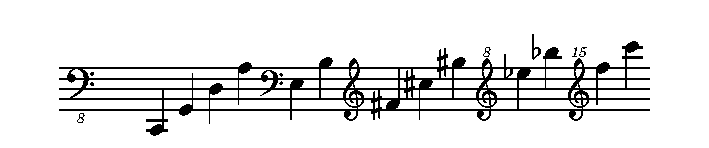
\includegraphics{examples/12-fifths.pdf}
\caption{The circle of twelve fifths}
\end{figure}
After proceeding through twelve fifths from our starting C, the final C is seven octaves
above it.
\begin{figure}[h]
\centering
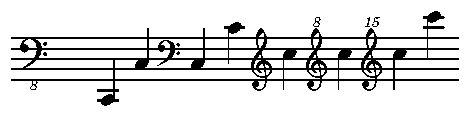
\includegraphics{examples/7-octaves.pdf}
\caption{The note C spanning seven octaves}
\end{figure}
If Pythagorean tuning was internally consistent, the C seven octaves above would be the
exact same pitch as the C resulting from twelve fifths. We can test this mathematically,
by adding together twelve ratios of 3:2 and comparing them with the sum of seven octaves
using the ratio 2:1.\autocite[25]{RD:1}
\begin{equation}
  \frac{3}{2} \times
  \frac{3}{2} \times
  \frac{3}{2} \times
  \frac{3}{2} \times
  \frac{3}{2} \times
  \frac{3}{2} \times
  \frac{3}{2} \times
  \frac{3}{2} \times
  \frac{3}{2} \times
  \frac{3}{2} \times
  \frac{3}{2} \times
  \frac{3}{2} = \frac{531441}{4096} = 129.7463
\end{equation}
\begin{equation}
  \frac{2}{1} \times
  \frac{2}{1} \times
  \frac{2}{1} \times
  \frac{2}{1} \times
  \frac{2}{1} \times
  \frac{2}{1} = \frac{128}{1} = 128
\end{equation}
The mathematical result is that the sum of the twelve fifths is greater than the sum of
the seven octaves. If we were to listen to these two pitches, they would not match.
The pitch resulting from twelve fifths above our starting C is noticeably sharper than 
the pitch resulting from seven octaves above the same starting note.

The additional problem with Pythagorean tuning was that it did not accurately reflect the pitches in the harmonic
series. The first three pitches in the harmonic series matched Pythagorean ratios perfectly. The pure intervals of the
octave, fifth, and fourth in the harmonic series were exactly in tune when compared to the ratios of their Pythagorean
counterparts. However, the fourth pitch in the harmonic series, the major third, when tuned acoustically pure as it
naturally occurred in the series, actually vibrated at a ratio of 5:4 and not 81:64, as the Pythagoreans would have
calculated by adding together two of their 9:8 wholetones: $ 9:8 \times 9:8 = 81:64 $.

These two tuning discrepancies that result from using only Pythagorean intervals to build a scale of notes are called
\textit{commas}. The \textit{ditonic comma} results when building a chromatic scale upon successive fifths, such as the
difference between twelve fifths and seven octaves, and the \textit{syntonic comma} results from the difference between
the pure harmonic 5:4 major third and the Pythagorean 81:64 major third. The Pythagoreans themselves were well aware of
these problems and tried to overcome them, but it was only Aristoxenus and Ptolemy who could offer a solution.
Aristoxenus proposal was to ignore the Pythagorean ideals of mathematical simplicity and use tuning systems that divided
the string according to parts and not ratios. He described tuning by using equal parts of the string and was the first
to develop the concept of tuning using equal semitones which would later be the foundation of equal temperament.
Ptolemy's proposal was to modify the Pythagorean notion of ratio by using only ratios that were superparticular in
nature, meaning that the first number of the ratio should always be one unit great than the other. So Pythagorean
ratios like 2:1, 3:2, 3:4 and even 9:8 were acceptable, but so too were other ratios such as 5:4, the pure major third,
and 6:5, the pure minor third.

Ptolemy's solution rectified a lot of the Pythagoreans' mathematical ratios with nature's
own internal tuning system but it still had problems when it came to musical execution.
In a twelve-tone scale, there are three major thirds. Starting on the note C, we can fit
three of them within an octave: C to E, E to G$\sharp$, and A$\flat$ to C.
\begin{figure}[h]
\centering
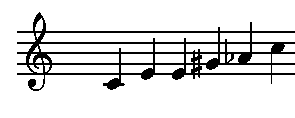
\includegraphics{examples/thirds.pdf}
\caption{Three major thirds within an octave}
\end{figure}
However, adding these intervals together using Ptolmey's ratios does not get us to a
complete octave either. The sum of three thirds should sound the same as an octave with
the ratio 2:1, but the mathematical result is slightly less than 2, which sounds flat.
\begin{equation}
  \frac{5}{4} \times
  \frac{5}{4} \times
  \frac{5}{4} \times = \frac{125}{64} = 1.953125
\end{equation}
While the note E could remain fixed in relationship to the major third starting from C and
the major third ending on G$\sharp$, the fact that G$\sharp$ and A$\flat$ are used for the other
two major thirds implies that they are different notes. Most modern musicians regard the
enharmonic respelling of a note as a kind of music homonym: an alternative word to express
the same thing. While the different names of G$\sharp$ and A$\flat$ can indicate different
functions, such as the third degree of the E major scale or the first degree of A$\flat$
major, they are regarded today as notes having the same vibrating pitch. However, as
Ptolemy's tuning problem shows us, the two notes are not only functionally different, they
are musically different, and therefore tuned differently.

Ptolemy's solution of tuning with only pure intervals is known as just intonation. While it succeeded in correcting the
problems associated with Pythagorean tuning, it made it impossible to tune certain notes in the chromatic scale because
they required a different tuning according to the musical context in which they occurred. Instruments of fixed pitches,
such as any keyboard instrument or fretted instrument, whose semitones were fixed and immobile, could not accommodate a
tuning of only pure intervals, or at least, not in a scale of twelve tones. Instruments of variable pitch, such as
fretless bowed instruments, wind instruments, or the human voice were exempt from this problem because they were able to
adjust any note appropriately. Violinists, for example can place their fingers at any position along the fingerboard,
and wind players may vary the pitch of their notes using their embouchure.

What about Aristoxenus? While he did invent an alternative solution of equal semitones, he rejected both the notions of
Pythagorean numeric purity and the Ptolemaic notion of harmonic purity. His method of tuning divided an octave into
equal parts, creating intervals as groups of these individual parts instead of using ratios. His idea of equal parts
formed the basis for equal temperament. While this allowed for a tuning of fixed pitches in a chromatic scale, none of
these intervals was tuned in a way that precisely matched the tuning in the harmonic series. This was an unacceptable
solution for most theorists and musicians during the evolution of western classical music, and it took many years for
equal temperament to gain acceptance.

Because the notion of equal semitones did not sit well with early western music theorists and tuning harmonically pure
intervals was impossible in a fixed pitch system, they gravitated towards the Pythagorean system of tuning. For one
reason, it was simple, using a small number of simple ratios, and for another, it matched the musical tastes of the
medieval period such as monophonic chants and polyphonic forms based on fifths, unisons, and octaves. Pythagorean
ratios persist even to this very day, but as music changed in the early Renaissance period, composers sought to
incorporate more consonant thirds into their music, which the strict Pythagorean system of ratios did not permit. Thus,
the old Greek debate between Pythagoras, Ptolemy, and Artistoxenus resurfaced.

\section{Temperament}

A temperament is a method of tuning a scale that alters an existing system, usually Pythagorean tuning. For most of the
Middle Ages, tuning was described according to the ratios that Pythagoras had determined hundreds of years earlier.
However, as musical tastes changed during the Renaissance, there was an increasing preference for the sounds of thirds
instead of unisons and fifths. This represented the problem of rectifying thirds within the Pythagoran tuning scheme
that had plagued the Greeks. The first attempts at a solution appeared at the end of the fifteenth century, and each one
used the same approach by changing the size of the fifths within the existing Pythagorean system.

One of the first writers to publish a system that broke with the Pythagorean tradition of tuning was Bartolomeus Ramis
de Pareja. In his \textit{Musica Practica} of 1482, he created a chromatic scale using two different groups of fifths.
Each group was tuned in pure fifths, just as in Pythagorean tuning, except that one group was slightly sharper than the
other. \autocite[88]{MB:1} Although he did not call it a temperament, it technically was not Pythagorean tuning either.
Barbour credits Franchinus Gafurius's \textit{Practica musica} of 1496 with the first mention of the idea of
temperament. In it, Gafurius says that organists tune their fifths slightly flat, but does not go into any specific
details.\autocite[25]{MB:1} Similarly, Arnolt Schlick's 1511 treatise \textit{Spiegel der Orgelmacher und Organisten}
only gives us a general idea when he refers to tuning the instrument's fifths flat 
``as much as the ear will permit.''\autocite[202]{RR:1} So while the idea was present as early as 1482, it took 
several years for it to develop into a system.

Tempering is a process of compromise whereby the acoustical purity of one interval is changed slightly in order to
accommodate the acoustical impurity of another interval. Specifically, it is the process of changing the size of the
fifth in order to accommodate the major third which is not pure in standard Pythagorean tuning. This usually means
shrinking the size of the fifth slightly so that it is narrower, or flatter than the pure ratio of 3:2; although, in
some cases a fifth may be tuned wider, or sharper than pure. The problem with Pythagorean thirds was that they were much
sharper than pure, differing by the syntonic comma, which was the difference between the Pythagorean third at 81:64 and
the pure harmonic third at 5:4. Shrinking the size of the fifth resulted in thirds that were flatter than the
Pythagorean ratio of 81:54, closer to the harmonically pure ratio of 5:4, and thus more appropriate sounding for music
that favored a greater number of thirds. Depending on how the fifth was flattened, you could come very close to a pure
5:4 third, and the listener would not notice the difference. This was at the expense of the fifth, which was now
flatter than pure, but it was an acceptable compromise because a flat fifth was less disconcerting than the sharp third
of Pythagorean tuning. The strategy was to shrink several fifths by the same or differing amounts. The result was that
instead of one set of intervals being completely pure and another unusable, all of the fifths were slightly out-of-tune
to differing degrees, while some of the thirds came very close to pure. Which thirds approached pure and which fifths
were made flat all depended on the particular temperament, and there were many!

Murray Barbour classifies temperaments into four basic types: regular meantone, irregular temperaments, equal division,
and equal temperament. Whereas a tuning can be defined as a method of obtaining intervals according to Pythagoras---as
in Pythagorean tuning---or according to Ptolemy---as in just intonation---temperaments alter the ratios of the intervals
so that they often lie somewhere between the two systems. In regular meantone temperaments, most or all of the fifths in
the Pythagorean tuning system are tuned flat by the same amount. Depending on which fifths are flattened, this can
result in thirds that are very close to pure, with fifths and fourths that are not. The amount that each fifth was
changed from its pure ratio often depended on the musical context. A meantone temperament with very flat fifths
resulted in a temperament with thirds quite close to pure, but because of the mutated nature of the fifths, it was
usable only in a limited number of keys. Conversely, a meantone temperament that tuned its fifths less flat made more
keys playable, but resulted in sharper, less pure thirds.

\subsection{Regular Meantone and Irregular Temperaments}

The first attempts at a systematic application of tempering fifths resulted in the class of temperaments known as
``meantone.'' No one is entirely sure who invented the first complete meantone temperament, but the general consensus
is that it is a shared prize between Pietro Aron and Gioseffo Zarlino. Zarlino is credited with the invention of an
exact system that narrows each fifth by $\frac{2}{7}$ of a syntonic comma. His method, however, was far from practical.
Although he provided a monochord diagram, his process of tempering the fifths by that much actually created thirds that
were smaller than pure, or too flat.

Pietro Aron is credited with the first practical meantone temperament. While not as theoretically exact as Zarlino's,
Aron's instructions can be used to create a workable meantone temperament that narrows fifths enough to create pure
thirds, while leaving the remainder of the intervals usable. Unlike Zarlino, his instructions are not mathematical in
nature, requiring the person to tune by ear and not rely on measurements. His method was to start with pure thirds and
build tempered fifths around them. He begins with a pure third between C and E and then proceeds to tune four fifths
that are all equally flat with additional pure thirds between A and C$\sharp$, and D and F$\sharp$. While Aron says
nothing about the division of the comma, Barbour takes these instructions and mathematically proves that if the tuner is
able to create Aron's pure thirds by ear and match the size of the other fifths so that they are all tempered by the
same amount, each of those fifths will be flatter than pure by $ \frac{1}{4} $ of a syntonic comma.\autocite[27]{MB:1}
Because this is the amount that each fifth is reduced in size, Aron's temperament is referred to as ``quarter-comma
meantone temperament.'' While Aron never referred to it this way, nor did he use mathematics to calculate lengths of a
string, later theorists and musicians adopted his ideas and made exact calculations that reproduced Aron's temperament.

Regular meantone temperaments contained eleven fifths that were all narrowed by the same amount, measured as a fraction
of the syntonic comma. Narrowing four consecutive fifths in the circle of fifths by $ \frac{1}{4} $ of a syntonic comma
was enough to make eight thirds in a 12-tone scale pure while rendering the remaining four unusable.\autocite[33]{RD:1}
This was an effective solution for sixteenth-century music because it resulted in more serviceable keys than Pythagorean
tuning, and composers simply avoided the keys containing the unusable thirds. This meant that meantone did not solve all
of the problems associated with Pythagorean tuning. Just as Pythagorean tuning has a fifth that was too wide to be
used, meantone temperaments also had an unusable fifth. The so-called ``wolf'' fifth existed in every temperament, but
its size and location depending on the kind of temperament.

As the sixteenth century continued, musicians attempted to correct the problems with quarter-comma meantone, such as its
wolf fifth and unusable thirds. These tuning systems narrowed the fifth in smaller amounts, such as $ \frac{1}{5} $ or
$ \frac{1}{6} $ of a syntonic comma. The result was that the thirds were now sharper than pure but much less so than in
Pythagorean tuning. While this created more usable thirds in the scale, the wolf fifth remained. Sixth-comma meantone
was popular with fretted instruments, as we will see in a later chapter, but even sixth-comma still contained the wolf
fifth and unequal thirds.

The next major change in temperaments occurred in the seventeenth century when theorists began using systems that
narrowed fifths by varying amounts instead of equal amounts, as was the case with regular meantone temperaments. So
called irregular temperaments, or well temperaments, became very popular and widespread in the seventeenth and
eighteenth centuries. The advantage to using well-temperaments was that musicians had finer control over which
intervals were problematic. For example, in quarter-comma meantone, the fifth between E$\flat$ and A$\flat$ is always
too wide to be used. Technically, this is because the A$\flat$ is really a G$\sharp$. \autocite[35]{RD:1} Similarly,
the thirds B to D$\sharp$, D$\flat$ to F and F$\sharp$ to A$\sharp$ would also be unacceptable. With irregular
temperaments, fifths were narrowed by differing amounts so that the wolf fifth was eliminated, and normally problematic
thirds in standard quarter-comma meantone could be made more tolerable by adjusting the size of other intervals instead.
These irregular temperaments were similar to regular meantone temperament, except that one fifth might be narrowed 
one-quarter of a comma, while another might be narrowed only by a sixth or less. As a result, the composer had more 
control over which keys had better-sounding thirds and which did not.

The introduction of irregular temperaments caused an explosion in the number and variety of temperaments available to
musicians in the seventeenth and eighteenth centuries. Theorists such as Valloti, Young, Werckmeister, and others all
developed their own systems of temperament favoring different intervals in ways that regular meantone temperaments could
not. Composers also developed their own temperaments as well, such as J. S. Bach who used his own temperaments in the
performance of his keyboard works. His compositions in \textit{The Well-Tempered Clavier} were so named because of the
temperament he used for them that allowed use of all keys on the instrument.

\subsection{Equal Division}

All of the methods described thus far are practical ways to create temperaments. For example, Aron's method uses the ear
alone and produces a good quarter-comma meantone temperament without the need for complex mathematical calculations.
Later methods of tuning other meantone temperaments and well-temperaments used the same techniques of narrowing or
widening intervals by certain amounts, either by ear or by some process of calculation.

The problem with some of these methods is that they are imprecise. The fifth is narrowed by an indeterminate amount to
match a pure third, or intervals are determined by counting the number of beats that occur as pitches clash against one
another. Most importantly, the resulting temperaments contain semitones that vary in size according to the placement of
the tempered intervals. If we are to compare different temperaments and their specific pitches, we need a more exact way
of calculating a given pitch in a given temperament.

Recalling Aristoxenus in our survey of Greek tuning methods, his approach consisted of dividing a string or octave into
equal parts and creating intervals by grouping tones into sets of these equal parts. Using this same method, we can
create several different regular meantone temperaments by dividing our octave into multiple parts and combining
wholetones and semitones into a groups. We can then accurately compare and quantify the size of each semitone across
different kinds of temperaments. Barbour refers to this process of calculating temperaments as equal division. Equal
division was used in the sixteenth century to calculate string lengths for both quarter and sixth-comma meantone, and
its principles remained in use into the seventeenth and eighteenth centuries.

The first theorist to use equal division was Vicentino in 1555, who divided his octave into 31 parts using a harpsichord
that contained six ranks of keys. He was attempting to create a temperament like quarter-comma meantone, but instead
used the principles of equal division instead of Aron's tempered fifths. In order to create an octave of 12 tones out of
a total of 31 parts, he combined five parts in each wholetone and made semitones of two different sizes, a smaller
semitone with two parts and a larger semitone with three. The size of the semitone depended on where it occurred within
the scale. Musicians during this time were familiar with these differences in semitone size and referred to the larger
semitone as the \textit{major semitone} and the smaller semitone as the \textit{minor semitone}. The difference in size
between the two semitones was referred to as a comma. We should not confuse this with the diatonic or syntonic comma,
which are differences of pitch as well, but have no correlation in systems of equal division.

Vicentino's 31-part system solved the same kinds of problems that meantone temperament did and created pure thirds at
the expense of pure fifths. However, it had the added advantage of clearly indicating that semitones differed in size by
one comma. Other approaches to meantone temperament were less specific and would tune certain semitones to a midway
point between the wholetone it was dividing. This was usually reserved for the wolf fifth or the chromatic notes which
were less likely to be used. As musicians developed systems of equal division, they utilized keyboards that could
realize the distinction between semitones more accurately and used split keys that enabled one to play either diatonic
or chromatic semitones. The use of enharmonic instruments that had more than twelve notes per octave dates back to the
late fifteenth century, and Patrizio Barbieri's recent book documents them extensively.\autocite{PB:1} Vicentino's
multi-manual keyboard was one example of such an instrument, but was too impractical to use. More practical examples of
keyboards with split keys were found later in the seventeenth century, especially in Italy. These instruments had
different keys for some or all of the accidentals; composers and keyboardists such as Handel and Werckmeister continued
to use them into the eighteenth century. \autocite[108]{MB:1}

Examining the 31-part system in more detail, let us take the C major scale as an example containing
five wholetones: C, D, F, G, A; and two semitones: E and B. In our system, we reach 31 parts by
assigning 5 parts to each wholetone and 3 parts to each semitone in the scale. 
Figure~\ref{31-part-octave} shows the arrangement of each pitch in the scale according to its number of parts.
% 31 division octave
\begin{figure}[h]
\centering
\setlength{\unitlength}{1mm}
\begin{picture}(96, 30)
  %\put(0,0){\circle*{1}}
  %\put(96,0){\circle*{1}}
  %\put(0,30){\circle*{1}}
  %\put(96,30){\circle*{1}}
  \linethickness{.075mm}
  \multiput(2, 15)(3, 0){32}{\line(0, 1){4}}
  \linethickness{.5mm}
  % C
  \put(2,12){\line(0,1){9}}
  \put(0,24){$C$}
  % D
  \put(17,12){\line(0,1){9}}
  \put(15,24){$D$}
  % E
  \put(32,12){\line(0,1){9}}
  \put(30,24){$E$}
  % F
  \put(41,12){\line(0,1){9}}
  \put(39,24){$F$}
  % G
  \put(56,12){\line(0,1){9}}
  \put(54,24){$G$}
  % A
  \put(71,12){\line(0,1){9}}
  \put(69,24){$A$}
  % B
  \put(86,12){\line(0,1){9}}
  \put(84,24){$B$}
  % C
  \put(95,12){\line(0,1){9}}
  \put(93,24){$C$}
\end{picture}
\caption{The C major scale in a 31-part system}
\label{31-part-octave}
\end{figure} 
Five wholetones at 5 parts apiece makes 25 parts, and adding
the remaining semitones at 3 parts each gives us a total of 31: $ 25 + 3 + 3 = 31 $. Note that
semitones E to F and B to C have 3 parts as opposed to 2. As we divide our scale further into
chromatic pitches, each wholetone is divided into 2 and 3 parts. Semitones that are diatonic within
a scale, such as E and B in a C major scale, always contain 3 parts as opposed to 2. The smaller
semitone is reserved for chromatic notes that lie outside the scale. For this reason, the larger
semitone is sometimes referred to as the \textit{diatonic semitone} while the smaller of the two is
called the \textit{chromatic semitone}. Figure~\ref{31-part-octave-complete} shows the rest of our C
major scale divided into its chromatic and diatonic semitones. 
% 31 division octave
\begin{figure}[h]
\centering
\setlength{\unitlength}{1mm}
\begin{picture}(96, 30)
  %\put(0,0){\circle*{1}}
  %\put(96,0){\circle*{1}}
  %\put(0,30){\circle*{1}}
  %\put(96,30){\circle*{1}}
  \linethickness{.075mm}
  \multiput(2, 15)(3, 0){32}{\line(0, 1){4}}
  \linethickness{.5mm}
  % C
  \put(2,12){\line(0,1){9}}
  \put(0,24){$C$}
  % C#
  \put(8,14){\line(0,1){7}}
  \put(7,24){$C\sharp$}
  % Db
  \put(11,12){\line(0,1){7}}
  \put(9,7){$D\flat$}
  % D
  \put(17,12){\line(0,1){9}}
  \put(15,24){$D$}
  % D#
  \put(23,14){\line(0,1){7}}
  \put(22,24){$D\sharp$}
  % Eb
  \put(26,12){\line(0,1){7}}
  \put(24,7){$E\flat$}
  % E
  \put(32,12){\line(0,1){9}}
  \put(30,24){$E$}
  % F
  \put(41,12){\line(0,1){9}}
  \put(39,24){$F$}
  % F#
  \put(47,14){\line(0,1){7}}
  \put(45,24){$F\sharp$}
  % Gb
  \put(50,12){\line(0,1){7}}
  \put(48,7){$G\flat$}
  % G
  \put(56,12){\line(0,1){9}}
  \put(54,24){$G$}
  % G#
  \put(62,14){\line(0,1){7}}
  \put(60,24){$G\sharp$}
  % Ab
  \put(65,12){\line(0,1){7}}
  \put(63,7){$A\flat$}
  % A
  \put(71,12){\line(0,1){9}}
  \put(69,24){$A$}
  % A#
  \put(77,14){\line(0,1){7}}
  \put(75,24){$A\sharp$}
  % Bb
  \put(80,12){\line(0,1){7}}
  \put(78,7){$B\flat$}
  % B
  \put(86,12){\line(0,1){9}}
  \put(84,24){$B$}
  % C
  \put(95,12){\line(0,1){9}}
  \put(93,24){$C$}
\end{picture}
\caption{The chromatic scale in a 31-part system}
\label{31-part-octave-complete}
\end{figure} 
Chromatic semitones represent the shortest distance between two pitches, such as the
distance from C to C$\sharp$, but this is also the same distance as G descending to G$\flat$.
Likewise, the distance ascending from C to D$\flat$ is the larger diatonic semitone, as well as the
descending distance from G to F$\sharp$. The term diatonic semitone might be misleading since it
implies that D$\flat$ or F$\sharp$ are diatonic to a C major scale. For this reason, the minor and
major designations are preferable.

Systems of equal division were not limited to just 31 parts. Zarlino and Salinas
describe a 19-division octave in the sixteenth century, and later systems included
octaves divided into 43 and 55 parts. Each of these systems grouped their wholetones
into an odd number of parts and therefore had their semitones divided unequally with a
comma's difference between them. Praetorius, in his \textit{Syntagma Musicum}, describes
a 55-part system with nine parts per wholetone and semitones of four or five parts. He
describes this system in reference to the ``intermediate'' nature of the semitones on
fretted instruments:
\begin{blocks}
Thus the semitones cannot be either major nor minor, but are, perforce, ``intermediate''
if anything. For I reckon that each fret [...] contains four-and-a-half commas, whereas
the major semitone contains five and the minor semitone only four. Since the error is
only half a comma either way, the ear hardly notices it with these instruments [...]
Major and minor semitones are both produced by the same fret, both sound in tune, [...]
especially since by particular applications of the finger to the string, over the fret,
it is possible to have some control over the pitch of the note produced.
\autocite[68]{MP:1}
\end{blocks}
As late as 1723, singer and teacher Pier Francesco Tosi expressed the same idea, though
not in reference to fretted instruments, in his treatise \textit{Opinioni de Cantori}:
\begin{blocks}
A Tone, that gradually passes to another, is divided into nine almost imperceptible
Intervals, which are called Commas, five of which constitute the Semitone Major, and four
the Minor.
\autocite[20]{PFT:1}
\end{blocks}
Praetorius and Tosi are both describing a system of equal division. Tosi was writing in
the eighteenth century, but equal division as a tuning method had already been in use
since the sixteenth century when it was used to mimic the same features of quarter-comma
meantone.

The basic features of each of these systems is outlined in table
~\ref{table:equalDivision}, where the corresponding meantone temperament is given. Of
the four that are listed, quarter-comma and sixth-comma are the most significant
because they were the most frequently used of the meantone systems.
\begin{table}[h!]
 \begin{center}
 \scalebox{0.7}
 {
  \begin{tabular}{ c c c c c}
   Number of Divisions & Wholetone & Major semitone & Minor semitone & Meantone equivalent \\
   \hline
   19 & 3 & 2 & 1 & third-comma meantone \\
   31 & 5 & 3 & 2 & quarter-comma meantone \\
   43 & 7 & 4 & 3 & fifth-comma meantone \\
   55 & 9 & 5 & 4 & sixth-comma meantone \\
   67 & 11 & 6 & 5 & seventh-comma meantone \\
   79 & 13 & 7 & 6 & eighth-comma meantone \\
  \end{tabular}
 }
 \end{center}
 \caption{Comparison of systems of equal division}
 \label{table:equalDivision}
\end{table}
Quarter-comma was used almost exclusively by keyboard and wind instruments, and was the
same kind of temperament that Vicentino was advocating with his system. Sixth-comma was
the same temperament that Praetorius, and later Tosi, were describing although
neither refer to it by that name. I will return to Praetorius's observation about
sixth-comma temperament when we examine other specific temperaments for fretted
instruments.

Although they each have different parts, each of the above systems function the same way as Vicentino's original
31-division octave. In a 19-division octave, wholetones consist of three parts, and major and minor semitones are two
and one parts respectively. 43-part systems contain wholetones with seven parts each, dividing their semitones between
four and three parts, and then a 55-part system has nine parts for its wholetones, divided into five and four. Other
systems were possible that created seventh and eighth comma meantone; however, these were not used to any great extent
since their tunings began to approximate equal temperament, and from a practical standpoint, did not serve as good a
purpose.

\subsection{Equal Temperament}

Technically speaking, equal temperament is a type of division in which the octave is divided into twelve equal parts.
In terms of its qualities as a temperament, it compensates for the ditonic comma the same way a meantone temperament
does by narrowing the fifth. The difference between equal temperament and meantone temperament is that meantone will
narrow its fifths much more than that. In equal temperament, all twelve fifths of the scale are narrowed by a slight
but equal amount. The ditonic comma is therefore dispersed throughout the entire scale so that every pitch is usable,
but this ability has its price. The temperament creates thirds that are as sharp as they possibly can be without having
too strong an effect on the listener. While they are not as sharp as the thirds of Pythagorean tuning, they lack the
pure quality of a quarter-comma meantone temperament and are too sharp to approximate it in the way that other meantone
and irregular temperaments do. However, the homogeneous nature of every third being sharp by the same amount tends to
veil this lack of harmonic purity from our ears, so that it is not as noticeable.

Even with its overly sharp thirds, theorists in the sixteenth century regarded equal
temperament as a technical impossibility. Because everyone based their tunings on the
Pythagorean 9:8 wholetone, it was mathematically impossible to divide it into two
geometrically equal, whole-number ratios. They could only divide the wholetone
unequally into a larger semitone of 17:16 and a smaller one of 18:17.
\autocite[20]{ML:1} If we recall that adding two geometrical ratios together requires a
process of multiplication, when 18:17 and 17:16 are ``geometrically'' added
together, it produces the 9:8 ratio.
\begin{equation}
 \frac{18}{17} \times
 \frac{17}{16} =
 \frac{306}{272} =
 \frac{\frac{306}{34}}{\frac{272}{34}} =
 \frac{9}{8}
\end{equation}
The difference between the two ratios is similar to the same differences in semitone size
found in meantone temperaments and systems of equal division. The smaller 18:17 ratio is
the minor semitone and the larger 17:16 ratio is major semitone.

Although equal temperament was impossible according to geometry, musicians knew how to approximate it very closely
without having to worry about the mathematics. Despite this ability, almost everyone preferred meantone temperaments
because of their pure thirds. Even later in the seventeenth and eighteenth centuries, irregular temperaments were still
favored over equal temperament because they made more keys feasible and were able to produce some thirds that were much
closer to pure than their equally-tempered counterparts.

A tuning method very similar to equal temperament appeared in Giovanni Maria Lanfranco's \textit{Monocordi \& Organi} of
1533. His system does not attempt to divide the octave into twelve parts, but instead mimics the quality of the fifth
found in systems that do. He describes a system where the fifths are tuned slightly flat and the thirds are made as
sharp as the ear can possibly endure. \autocite[45]{MB:1} Other writers after him described the same kind of system,
sometimes giving him credit and sometimes not. Although Lanfranco's temperament made it possible to use more pitches of
the chromatic scale, just as equal temperament does, it still created overly sharp thirds making it inferior to meantone
temperament at the time.

One of the first systems to create equal temperament using measurable means was known as the \textit{18:17 rule}. The
theorist and lute player Vincenzo Galilei is credited with developing it for practical use. \autocite[57]{MB:1}
Although technically not true equal temperament, Galilei created twelve semitones of the same size in an octave using a
series of Pythagorean minor semitones, or the smaller ratio of the 9:8 wholetone, the 18:17 semitone. His procedure was
relatively straightforward: A string is divided into 18 equal parts, and the first part or $ \frac{1}{18} $ of the
string, is marked as the first semitone. The remaining length or $ \frac{17}{18} $ of the string is then redivided into
another 18 different parts. The first part of this division is then marked as the second semitone. The process is then
repeated with the remaining string length to mark the third semitone, and so on, each time redividing the remaining
amount of string into 18 parts and marking the first part as the next semitone.

Since the Pythagorean minor semitone is slightly smaller than an equally tempered semitone, Galilei's system was not the
same as modern equal temperament, but was a way to divide the octave into twelve working semitones. Since each
successive semitone is a bit flat, the fifth is slightly flat as well, very close to an equally-tempered fifth, with the
octave at the twelfth fret flat as well. This issue seemed to go unnoticed on fretted instruments because of the way in
which pitches tend to be sharper at higher frets. Since Galilei was a lutenist, he was using temperaments that he found
the best for his instruments. While this worked well for the lute, it did not apply to non-fretted instruments. The
same feature of sharp thirds still remained in Galilei's method just as it did with all other temperaments at this time
that approximated equal temperament.

Despite the predominance of meantone temperament in the sixteenth century, many shared Galilei's opinions and accepted
the fact that lutes and other fretted instruments should be tuned with equal semitones. These included such notable
musicians as Vicentino, Zarlino, Salinas, Artusi, Praetorius, and Mersenne. \autocite[19]{ML:1} This did not mean that
lutes were tuned in the same kind of equal temperament that we find today. As we will see later, there were variations
in which lutes and other fretted instruments approximated equal frets as well as making their frets unequal to match
common meantone temperaments.

Equal temperament was not fully accepted in musical practice until at least the eighteenth century, and even as late as
the twentieth. Ross Duffin provides ample evidence that musicians were tuning their fifths flatter than those in
today's equal temperament systems well into the nineteenth century, and that true equal temperament really did not
become a indisputable fact until 1917 when it was standardized. \autocite[138]{RD:1} After that, the advent of modern
electronic tuning devices that enabled tuners and musicians to calculate a correctly tempered fifth precisely,
solidified equal temperament's place in the modern musical world.

\section{Describing Temperaments}

Throughout the course of this study, we will need to refer to the qualities of the different temperaments explained thus
far as well as compare them to other lute-specific temperaments that we will encounter in later chapters. Audio
examples can illustrate the differences between temperaments, but sometimes they are so slight that even the most
trained ear might have difficulty in distinguishing them, or be unable to describe the difference accurately. For
example, it might be difficult for any of us to distinguish between a fifth that had been narrowed by one-fifth of a
comma and one that was narrowed by a sixth. Furthermore, comparing several different temperaments with audio examples
in the context of a written paper can impede the reader, and papers, of course, do not have speakers built into them.

Using numerical means to express temperaments is one of the ways to show the exact difference between intervals in a
written environment, and we can do this in several different ways. The first, which I have already used, describes
intervals as whole-number ratios, as the Greeks did thousands of years ago. This was also the way that most everyone
else did so in the sixteenth and seventeenth centuries. For that reason, I will use these whole-number ratios whenever
possible to refer to numerical differences between intervals. However, not all intervals are easily defined using these
kinds of ratios.

Meantone temperament uses intervals that can be expressed as whole number ratios, but these are not easily derived. We
can calculate the ratios of meantone intervals in two ways. The first involves determining the parts of a comma and
subtracting them from the fifth, as Aron originally suggested. The only difference is that Aron was using his ear to
achieve this, but here we will propose a second, more mathematic method to achieve the same result. Furthermore, we
shall also need to precisely articulate the differences of semitone and interval size in a variety of meantone
temperaments.

Because each system of meantone temperament has a matching system of equal division, we can express its intervals
mathematically with the same system of parts or commas that were used historically. For example, in Vicentino's 31-part
octave, the fifth would comprise three wholetones and a major semitone. Referring to figure~\ref{31-part-octave}, that
makes a total of 18 parts out of the total 31. We can calculate this as: $2^\frac{18}{31}$. Applying the same ratios
of parts as exponential fractions, we can calculate any interval in any meantone system, such as the quarter-comma major
semitone: $ 2^\frac{3}{31} $; or the sixth-comma major semitone: $ 2^\frac{5}{55} $. Incidentally, we can also express
intervals in equal temperament the same way.  The semitone in equal temperament is: $ 2^\frac{1}{12} $; the wholetone
$ 2^\frac{2}{12} $; the fifth: $ 2^\frac{5}{12} $ and so on. The obvious problem with these numeric representations is
that are more difficult to comprehend than a simple number, and are not readily comparable to standard Pythagorean
ratios.

In order to compare all these different kinds of semitones effectively, we need to
express either their ratio or their logarithmic formula as a simple decimal number. In
this case, the number could be applied to a string length to determine what length of
string would produce a sixth-comma meantone major semitone, a quarter-comma meantone
fifth, or a pure third, and it can also determine the vibrating frequency of those
particular pitches as well. Referring to table~\ref{fifth-comparison}, if we compare
the Pythagorean ratio 3:2 with its quarter-comma meantone equivalent, expressed using
logarithmic functions, we can immediately see that the Pythagorean fifth is slightly
larger. We also see that the quarter-comma third matches the ratio of the
pure third more closely, as opposed to the fifth or sixth-comma third.
\begin{table}[h!]
  \begin{center}
  \begin{tabular}{ r l }
    Pythagorean fifth:      & $ 3:2 = 1.500 $ \\
    Quarter-comma meantone fifth: & $ 2^\frac{18}{31} = 1.4955 $ \\
    \hline
    Pure third:          & $ 5:4 = 1.2500 $ \\
    Third-comma meantone third:  & $ 2^\frac{6}{19} = 1.2447 $ \\
    Quarter-comma meantone third: & $ 2^\frac{10}{31} = 1.2506 $ \\
    Fifth-comma meantone third:  & $ 2^\frac{14}{43} = 1.2532 $ \\
    Sixth-comma meantone third:  & $ 2^\frac{18}{55} = 1.2546 $ \\
  \end{tabular}
  \end{center}
  \caption{Comparison of pure and meantone fifths and thirds using decimal equivalents}
  \label{fifth-comparison}
\end{table}
We know from Aron's description of tuning meantone temperament that the fifth was
tuned slightly flatter than pure, and the chart also bears this out, with the
quarter-comma fifth smaller than the pure fifth.

The decimal equivalents I am choosing to express these differences do not have any musical significance. However, the
useful feature of these decimal numbers is that one can easily rank the different temperaments from smaller to larger,
or flatter to sharper. Larger numbers indicate a larger or wider interval that is sharp. Conversely, smaller numbers
indicate smaller or narrower intervals that are flat. With the ability to calculate any kind of semitone, whether
chromatic or diatonic, in any meantone temperament quarter-comma or otherwise, we can now correctly determine what kind
of temperament and semitones lute fretting systems used. That is the matter to which we now turn directly.

% Lute fretting systems

\chapter{Lute Fretting Systems}

In the previous chapter, I set forth several different methods in which we can measure
ratios of intervals to determine the quality of their temperament.  In this chapter, I
will apply these methods to different fretting schemes and determine, from a
mathematical standpoint, what kind of tempered interval each fret represents.  The
overall picture for lute temperaments from the sixteenth through early seventeenth
centuries can be outlined as follows: Pythagorean tunings were used exclusively at the
beginning of the period, and retained some use for certain intervals later in the
period. By the mid-sixteenth century, lute players began to add different types of
tempered intervals into the existing Pythagorean scheme.  Some of these intervals were
meantone, some approximating equal temperament, and others were original in their
quality.  From the end of century onward, fretting systems remained mixed, or else
used methods of dividing the octave into twelve equal semitones; however, their
semitones did not always match those of modern-day equal temperament. The important
distinction between these systems and keyboard temperaments at the time was
that lute temperaments did not fall completely into one kind of tuning or temperament
and were specific to the instrument.

The majority of instructions published during this period provided the player
with a practical means of setting frets and did not dwell on theory.  Almost all of the
sources have very precise rules for determining fret placement that use measuring tools
such as the straight-edge and compass.  These were commonly used for making
geometrical divisions, and when used to calculate fret placement, could
divide a line into any number of equal parts.  The remainder of the sources are less
precise and instruct the player to place a fret somewhere near another until it
sounds agreeable, or to move a fret slightly in one direction or the other, without
providing exact measurements.

What follows is a comparison of several fretting systems that appeared in lute and
vihuela treatises. For those sources that have instructions on placing frets using a
compass, I have determined the exact ratio of the interval using the arithmetic methods 
outlined in the previous chapter.  The details of the calculations can be found in
the appendix.

\section{Pythagorean Tunings for Lute}

Starting in the 9th century, most if not all fretted instruments were tuned according to
Pythagorean ratios.  The placement of frets on these instruments yielded pure fifths, fourths, and octaves
as well as wholetones with a ratio of 9:8. \autocite[9]{ML:1} The result of this, as we
saw in the previous chapter, was that major thirds were much wider than pure.  What we
know of the lute prior to 1500 suggests that it was a four- or five-stringed instrument
tuned in fourths.  Such a tuning would accommodate a Pythagorean tuning quite well, but
after 1500, the lute's repertoire changed and a sixth string was added.  The new tuning of
the 6-course lute used a minor third between the instrument's third and fourth courses
which exposes the major limitation of a Pythagorean system of tuning.

Because theory treatises in the early sixteenth century still advocated Pythagorean
systems of tuning because of its mathematical principles, lute players were left to
forge their own solutions to the tuning dilemma.  One of the mainstays of lute
repertoire throughout the sixteenth century was intabulated polyphonic music. The first
books of music printed by Petrucci in the early 1500s contain peices of this kind, and
composers of lute music would include many of
them in their publications. Because this music had many harmonies that relied on
thirds, a Pythagorean system of tuning would have presented some obvious shortcomings.
It is at this point that we see lute players begin a gradual shift away from
Pythagorean tunings and towards meantone temperaments.

During the first half of the sixteenth century, at least three different tuning methods
for lute were published.  Two of these kept with the existing Pythagorean tradition of
the day, while the third departed from that tradition and employed a kind of meantone
tuning similar to that which Pietro Aaron and Vicentino were developing at the. 
\textit{Epithoma musice instrumentalis}, published in 1530 by Oronce
Fin\'{e}, was one of the sources that retained Pythagorean principles.  Fin\'{e} was a
professor of mathematics at the University of Paris and mostly published theoretical
works about mathematics. It was his personal interest in music that compelled him to
write \textit{Epithoma}. Written in Latin, the book includes instructions for tuning a
lute, reading tablature and setting frets of a lute.  Pierre Attaingnant was a friend
of Fin\'{e}'s and it was probably this friendship that resulted in the treatise's
publication.  An additional set of lute instructions appear in Attaignant's publication
\textit{Tres breve et familiere introduction pour entendre et apprendre [...]} in 1529,
this time written in French.  Some stipulate that these were instructions from Fin\'{e}
and just translated, but this has never been fully proven.\autocite[1]{PV:1}

Another example of Pythagorean tuning appeared in a book published about the middle of
sixteenth-century.  The book was not about music but instead contained various topics
concerning France.  Appearing in 1556 and carrying the long title of \textit{Discours non
plus melancoliques que diverses, de choses mesmement, qui appartiennent a notre FRANCE: \&
a la fin La maniere de bien \& iustement entoucher les Lucs \& Guiternes}, it has been
attributed to Bonaventure des Periers, but some sources list it as an anonymous author.
The subject of tuning lutes and guitars appears in the last chapter of the book, which,
curiously, has nothing to do with any of the other chapters in the book. The final chapter
of \textit{Discours [...]} contains instructions for fretting and tuning these instruments
as well as a diagram of a mesolab, an ancient geometric tool that was first used to solve
the problem of dividing a string into equal semitones.

In his assessment of their fretting instructions, Mark Lindley has concluded that Both
Fin\'{e} and the anonymous \textit{Discours [...]}  preserved the same characteristics of
other Pythagorean tuning methods.  These included earlier theorists from the fifteenth
century such as Henri Arnaut, Johannes Legreze, Nicola Burzio and Franchino Gafurio, as
well as more contemporary theorists like Heinrich Schreiber of Erfurt and Pietro Aron
\autocite[11]{ML:1}. The features of these fretting schemes resulted in fourths and fifths
at ratios of 4:3 and 3:2 respectively, and wholetones with a ratio of 9:8.  Semitones
depended on which fret the measurements began.  In \textit{Discours [...]}, frets 2, 4 and
6 were a series of 9:8 ratios beginning with the nut, while frets 1, 3, 5 and 7 were
series of 9:8 ratios beginning with the seventh fret and moving backwards.  Fin\'{e}'s
method was slightly different, placing frets 6, 8 and 10 at 9:8 ratios starting from the
twelfth fret.

The inherent problem with these systems is that the fret placement is based purely on
mathematics and maintaining Pythagorean ratios without any deference to practical
musicianship. Fin\'{e} was not a musician, and Lindley suggests that that the author of
\textit{Discours [...]} was not either \autocite[11]{ML:1}.  Furthermore, after
attempting to play various pieces from the period, he concludes that ``it seems
doubtful to me that sensitive players would really have left the pythagorean scheme
unaltered.'' \autocite[13]{ML:1}  This becomes apparent in later sources from Juan
Bermudo and Sylvestro Ganassi who each began with a Pythagorean tuning scheme and then
adjusted it to make it more palatable.

Successive instructions on fretting from the mid-sixteenth century onward de-emphasized
Pythagorean systems in favor of tempered intervals and methods of equal fretting.
While they certainly acknowledged Pythagorean intervals, and writers such as Bermudo
and Ganassi offered complete fretting systems using Pythagorean ratios, they were never
intended to be the final solution. Most musicians recognized the importance of
Pythagorean intervals, such as the fourth, fifth, octave and in some cases the
wholetone; however, they also used non-Pythagorean intervals to create a better
solution.  The primary distinction between sources that advocated Pythagorean tuning
over a tempered kind was that Pythagorean sources tended to focus more on
mathematical issues than musical ones.


%
% Hans Gerle
%
\section{Gerle's fretting instructions}

The first major break with Pythagorean systems of tuning for lute came from Hans Gerle, a
lutenist and composer who published his treatise in 1533.  In addition to its specific
explanation of fret placement, it is also one of the best sources for lute instruction and
practice in the early sixteenth century.  It contains detailed explanations of tuning,
right-hand and left-hand technique as well as tablature.  The most important feature of
Gerle's treatment of lute fretting, and the others that I will be analyzing in this
chapter, is that Gerle was a lute player and not a theorist. From this viewpoint, matters
of theory are discarded in favor of practicality.  Gerle probably knew very little of the
implications of breaking with the tradition of Pythagorean tuning.  His emphasis was on
finding a practical way to fret the lute in such a way that it would sound agreeable.  The
importance of his instructions become more apparent when we see other lutenists such as
John Dowland borrowing many of Gerle's methods over 75 years later.

Gerle's instructions are directed towards a player who may or may not have theoretical
knowledge of music, but would have had some rudimentary knowledge of arithmetic and
geometry.  His process involved using a compass and a straight edge, such as a piece of
wood or other material that the player cuts to be the same length as the vibrating string
length of the instrument.  Marks were made on the straight edge, using the compass to
divide the distances between each mark into different parts.  Once all the appropriate
marks were made, they could be transferred to the fretboard and the frets placed
accordingly.

He uses a very straight-forward, step-by-step approach for setting each fret, beginning
with the twelfth.
\begin{blocks}
Take a straight-edge that is thin or else a flat piece of wood like a ruler, and make it
of such a length that at the top it touches the piece of wood that the strings lie on and
also touches the bridge that the strings lie on, and when you have made the ruler so that
it touches at both ends (don't make it too short; it must touch as I have said), mark the
bottom part at the bridge with an a, and the top part with a b, so that you will know
which end belongs to the bridge.  Then lay the ruler on a table, and take a compass and
find the middle of the ruler.  Mark it with a point or little dot and put an m there.
\end{blocks}
The letter \textit{a} marks the bridge and the letter \textit{b} marks the nut.
By placing the twelfth fret in the middle of the string, he divides the string in half
yielding $ \frac{1}{2} $, or in terms of a ratio, this would be an octave of 2:1.
Compasses were widely used at this time to perform all kinds of geometrical divisions and
we can assume most learned individuals at this time would know how to use one in order to
execute Gerle's instructions.  Euclid, the Greek mathematician, described procedures for
dividing lines into equal parts in his famous work \textit{Elements}.  This book was
first translated into Latin in 1482 and appeared in English translation by 1570.  Although
Gerle was German, it is reasonable to assume that he could have had access to either a
copy in Latin or one in German.  As far was we know, Gerle was not educated at a university
and probably had little or no knowledge of Latin; however, it is still reasonable to
assume that with Euclid's work in circulation, he could have come by the knowledge needed
to perform the required geometrical calculations.

% Gerle's seventh fret
Gerle continues using pure intervals for the fifth, or seventh fret:
\begin{blocks}
Then divide from the m to the b [in] three parts; and the first part from the m gives you
the seventh and lowest fret.  Mark it with a dot and put the number 7 there.
\end{blocks}
The letter \textit{b}, marked in the previous step, denotes the nut at one end of the ruler.
Gerle now switches to numbers for frets and indicates the seventh fret with the number 7.
The fret is marked at the first of the three parts starting from the twelfth fret or
middle of the string.  The resulting fret placement is one-third the length of the string,
making the vibrating length of the remaining string two-thirds. We can express this
semantically as a string divided into three parts with a vibrating length of two parts, or
3:2, which corresponds to the pure fifth.  Gerle could have divided the entire string into
three parts and placed the seventh fret at the first part from the nut, but it seemed more
important to base successive frets on the location of existing ones, in this case, the
twelfth.

% Gerle's first fret
Gerle's instructions continue with the first fret, and similar to his instructions for the
seventh, he builds on the calculations of the previous fret to find its location.
\begin{blocks}
Then divide elevenfold from the number to the b, and two of the same parts down from the b
give you the first fret.  Mark this also with a dot and put the number 1 there.
\end{blocks}
The ``number'' he is referring to is seven, or the seventh fret that we just marked in the
previous step.  Here he has us divide the distance from the nut to this fret in eleven
parts and mark the second of these parts starting from the nut. This creates a ratio of
33:31, which is not Pythagorean but instead somewhere between the diatonic semitone
16:15 and the ratio 17:16. Mark Lindley has determined that this distance is actually a
one-sixth comma semitone, but what kind?  In chapter two, we examined systems of equal
division that divided the octave into multiple parts greater than twelve.  Sixth-comma
meantone corresponded to an octave divided into 55 parts, and the first fret on the lute
would be the first semitone in a 55-division system.  If the semitone is chromatic, 
it has four parts, and if it is diatonic, it has five.

To determine which semitone Gerle was using we can compare our calculations of his fret
distance with the known values of different semitones.  If we express Gerle's 33:31 ratio
as a decimal by dividing 33 by 31, we get $ \frac{33}{31} = 1.0645 $ rounded off
to the nearest fourth decimal place.
\begin{table}[h!]
    \begin{center}
    \begin{tabular}{ r l }
        Equal temperament semitone:     & $ 2^\frac{1}{12} = 1.0600 $ \\
        Sixth comma chromatic semitone: & $ 2^\frac{4}{55} = 1.0517 $ \\
        Sixth comma diatonic semitone:  & $ 2^\frac{5}{55} = 1.0650 $ \\
    \end{tabular}
    \end{center}
    \caption{Equal and sixth-comma semitones}
    \label{table:6semitones}
\end{table}
Comparing that value to the values of other semitones in table ~\ref{table:6semitones}
we can see that Gerle's first fret matches the diatonic semitone in sixth comma
meantone temperament.

Gerle has departed from Pythagorean tuning and opted for a tempered semitone at the first
fret.  This is not to say that he is advocating a sixth comma meantone tuning overall.
Gerle still uses a pure fifth at the seventh fret, which is not the same as a
fifth tuned in sixth comma.  A sixth-comma fifth is slightly flatter.
\begin{table}[h!]
    \begin{center}
    \begin{tabular}{ r l l }
        Pure fifth:        & 3:2                 & $ = 1.5000 $ \\
        Sixth comma fifth: & $ 2^\frac{32}{55} $ & $ = 1.4967 $ \\
    \end{tabular}
    \end{center}
    \caption{Comparison of pure and sixth-comma fifths}
    \label{table:6fifths}
\end{table}
The fifth is comprised of three whole tones and one diatonic semitone. In a sixth-comma
system this makes up 32 parts or \textit{dieses}, and the resulting interval is slightly smaller
than the pure Pythagorean fifth, which is what we should expect in any regular meantone
temperament (see table ~\ref{table:6fifths}). This will have implications when we examine
the internal tuning issues of lutes later.

% Gerle's second fret
After having placed the first fret, Gerle continues with the placement of the second, or the whole tone.
Here, he returns to the standard Pythagorean 9:8 ratio:
\begin{blocks}
Then divide again from the number 7 to the b threefold, and the first part down
from the b gives you the second fret.  Mark it also with a dot and put the
number 2 there.
\end{blocks}
Here we have a three part division from the seventh fret to the letter \textit{b}, 
which was marked in the first step at the nut.
By returning to our earlier calculation of the seventh fret, we can formulate the
second fret distance and vibrating length accordingly which results in the Pythagorean
wholetone.

% Gerle's fifth fret
So far, Gerle has mixed Pythagorean pure intervals with tempered ones, such as
the fifth, the major second and the tempered minor second.  As he moves to the
perfect fourth at the fifth fret, he writes:
\begin{blocks}
Then divide from the m to the b in two parts, and the one part gives you the
fifth fret. Mark it with a dot and put the number 5 there.
\end{blocks}
Starting from the twelfth fret, Gerle divides the distance into two parts and takes the
first part from the nut as the mark for the fret. The letter m is our octave fret, the
exact midpoint of the string. Since he is now dividing that again in half, this
produces a Pythagorean interval of the fourth with a ratio of 4:3.

% Gerle's sixth fret
Now Gerle turns his attention to the tritone, or sixth fret:
\begin{blocks}
Then put the sixth fret in the middle of the fifth and seventh frets.  Make it
with a dot and put the number 6 there.
\end{blocks}
If we assume that Gerle is using ``middle'' to denote the arithmetic mean, as opposed
to the geometric mean, we can calculate the middle distance between the
fifth and seventh frets and get a vibrating ratio of 24:17.  However, an alternative
explanation is that Gerle is being intentionally vague here as if to tell the player to
put the fret somewhere between the two frets, and not necessarily exactly in the
middle.  If we assume this, then it seems reasonable to assume that the player
could also alter the placement until it produced a good result.

Regardless of our interpretation of Gerle's instruction, the tritone is neither
Pythagorean ratio nor sixth-comma meantone, but it may be close enough to be considered
equally tempered. In a sixth comma meantone with a 55-division octave, the tritone
contains either 27 or 28 dieses depending on whether the semitone above the
fourth is chromatic or diatonic.  For a lute tuned in G, this would be the difference
between a D$\sharp$ and an E$\flat$. Calculating the decimal equivalents for these two
semitones shows us that Gerle's tritone falls somewhere between the chromatic and
diatonic semitones.  Although this fret is not identical numerically to the
equally-tempered tritone, if we look at a scaled drawing depicting the location of the
fret in relation to the other intervals, Gerle's fret and the location of the
equally-tempered fret look nearly identical. We must note that Gerle places the fret in
the middle of the other two frets without the use of a compass.  Furthermore, while
Gerle's sixth fret may come close enough to equal temperament that we could call it an
equally tempered interval, he is not using equal temperament in the modern sense.  In
fact, Gerle was using meantone in its original sense, the way in which Aaron would have
tuned.

Meantone temperaments that did not use equal division had to approximate some of their
semitones by dividing the wholetone differently. For example, Aaron's
original instructions did not consider every semitone in the scale, it only covered a
set of thirds that were tuned pure leaving some of the other pitches indeterminate.
Semitones that were not included in the scheme were divided, splitting a wholetone into
two different parts. Since this was probably done by ear and without the aid of exact
measurements, the calculation of this fret is an approximation and we should discount
the use of arithmetic to determine the quality of the semitone between the fifth and 
seventh frets.

In order to better visualize frets that are approximations instead of
exact calculations, we can can look at a scaled drawing comparing the placement of
the different semitones.  I will be using many such scaled drawings and each will use
the same sample mensur length of 70 centimeters.  The purpose of the drawing is not to
show the exact placement of frets that would normally be approximate, but to
demonstrate how one type of inexact fret may be similar to another type of fret that is
exact in its placement by showing how close they are to another.  The choice of mensur
length is based on what best appears on the page.  While 70 centimeters is unusual for
a lute, a more common mensur length of 60 centimeters is smaller on the page and does
not exhibit the differences of semitone size as clearly.

In turning to Gerle's sixth fret, we can look at one of these scaled drawings comparing
his fret with the known placement of the chromatic sixth-comma semitone, the diatonic
sixth-comma semitone and the equally tempered semitone.  These frets are shown in red
while Gerle's frets are in black.
\begin{figure}[ht]
\centering
\setlength{\unitlength}{1mm}
\begin{picture}(60,68.3)
% Draw fingerboard edges
\color{black}
\linethickness{0.075mm}
\put(0,0){\line(0,1){68.3}}
\put(60,0){\line(0,1){68.3}}

% Draw strings
% 6th course
\color{strings}
\linethickness{0.5mm}
\put(5,0){\line(0,1){68.3}}
\linethickness{0.25mm}
\put(7,0){\line(0,1){68.3}}
% 5th course
\put(15,0){\line(0,1){68.3}}
\put(17,0){\line(0,1){68.3}}
% 4th course
\put(25,0){\line(0,1){68.3}}
\put(27,0){\line(0,1){68.3}}
% 3rd course
\put(35,0){\line(0,1){68.3}}
\put(37,0){\line(0,1){68.3}}
% 2nd course
\put(45,0){\line(0,1){68.3}}
\put(47,0){\line(0,1){68.3}}
% 1st course
\put(56,0){\line(0,1){68.3}}
\color{markers}
\linethickness{0.5mm}
\put(0,30.2){\line(1,0){60}}
\color{black}
\put(60,29.6){\tiny{\textemdash diatonic sixth-comma semitone}}
\color{markers}
\linethickness{0.5mm}
\put(0,33.3){\line(1,0){60}}
\color{black}
\put(60,32.7){\tiny{\textemdash equal semitone}}
\color{markers}
\linethickness{0.5mm}
\put(0,36.4){\line(1,0){60}}
\color{black}
\put(60,35.8){\tiny{\textemdash chromatic sixth-comma semitone}}
\color{black}
\linethickness{1mm}
\put(0,34.1){\line(1,0){60}}
\color{black}
\linethickness{1mm}
\put(0,63.3){\line(1,0){60}}
\color{black}
\put(60,62.3){\small{\textemdash 5th fret}}
\color{black}
\linethickness{1mm}
\put(0,5){\line(1,0){60}}
\color{black}
\put(60,4){\small{\textemdash 7th fret}}
\end{picture}
\caption{Scale drawing of Gerle's sixth fret}
\label{fig:gerle-6}
\end{figure}

Gerle's fret favors the chromatic side, although given the proximity of their
locations, his fret is very near the equally tempered semitone that it could be
considered closer. Another point to bear in mind is that as the mensur length
decreases, so will the distances between these frets.  Conversely, the distances will
increase as the mensur increases.  This will have more bearing on the theorbo, which
has a mensur length of 80 centimeters or more, and is discussed in later chapters where
I focus on executing different types of fret placements.

Gerle next instructs us where to place the third fret by taking a portion of the 
distance from the nut to the first fret.
\begin{blocks}
Then divide from the number 1 to the b [in] three parts, and when you have the
three parts then go with the compass unaltered down from the number 1 again five
spans; that gives you the third fret.  Mark it with a dot and put the number 3
there.
\end{blocks}
Gerle's uses the term ``span'' to denote one of the three parts in the distance from
the first fret to the net. Therefore, the total spans from the nut (b) to the third fret 
is eight: the five spans
from the first fret to the third, plus the original three spans from the nut to
the first fret.  The resulting 99:83 ratio is closest to a diatonic sixth comma
meantone minor third.
\begin{figure}[ht]
\centering
\setlength{\unitlength}{1mm}
\begin{picture}(60,45.4)
% Draw fingerboard edges
\color{black}
\linethickness{0.075mm}
\put(0,0){\line(0,1){45.4}}
\put(60,0){\line(0,1){45.4}}

% Draw strings
% 6th course
\color{strings}
\linethickness{0.5mm}
\put(5,0){\line(0,1){45.4}}
\linethickness{0.25mm}
\put(7,0){\line(0,1){45.4}}
% 5th course
\put(15,0){\line(0,1){45.4}}
\put(17,0){\line(0,1){45.4}}
% 4th course
\put(25,0){\line(0,1){45.4}}
\put(27,0){\line(0,1){45.4}}
% 3rd course
\put(35,0){\line(0,1){45.4}}
\put(37,0){\line(0,1){45.4}}
% 2nd course
\put(45,0){\line(0,1){45.4}}
\put(47,0){\line(0,1){45.4}}
% 1st course
\put(56,0){\line(0,1){45.4}}
\color{markers}
\linethickness{0.5mm}
\put(0,5){\line(1,0){60}}
\color{black}
\put(60,4.4){\tiny{\textemdash diatonic sixth-comma semitone}}
\color{markers}
\linethickness{0.5mm}
\put(0,6.8){\line(1,0){60}}
\color{black}
\put(60,6.2){\tiny{\textemdash equal semitone}}
\color{black}
\linethickness{1mm}
\put(0,40.4){\line(1,0){60}}
\color{black}
\put(60,39.4){\small{\textemdash 2nd fret}}
\color{black}
\linethickness{1mm}
\put(0,5.09999999999999){\line(1,0){60}}
\end{picture}
\caption{Scale drawing of Gerle's third fret}
\label{fig:gerle-3}
\end{figure}

In looking at the scale drawing, the black line representing the fret completely
occludes the red line of the diatonic sixth-comma semitone, indicating that for all
practical purposes the two semitones are the same.  Longer mensur lengths might exhibit
a slight difference in distance but it would be minimal.

The last fret is the fourth which makes the major third.  Similar to the sixth fret, he
averages the distance between the third and fifth.
\begin{blocks}
Then put the fourth fret between the third and the fifth frets.  Mark it with a
dot and put the number 4 there.
\end{blocks}
Averaging the distance between the two frets results in the ratio 792:629, which comes
closest to the equal tempered major third. Referring to a drawing of the fourth fret,
Gerle's major third is flatter than a true equally tempered third, but sharper than a
major third in a sixth comma temperament.
\begin{figure}[ht]
\centering
\setlength{\unitlength}{1mm}
\begin{picture}(60,71.9)
% Draw fingerboard edges
\color{black}
\linethickness{0.075mm}
\put(0,0){\line(0,1){71.9}}
\put(60,0){\line(0,1){71.9}}

% Draw strings
% 6th course
\color{strings}
\linethickness{0.5mm}
\put(5,0){\line(0,1){71.9}}
\linethickness{0.25mm}
\put(7,0){\line(0,1){71.9}}
% 5th course
\put(15,0){\line(0,1){71.9}}
\put(17,0){\line(0,1){71.9}}
% 4th course
\put(25,0){\line(0,1){71.9}}
\put(27,0){\line(0,1){71.9}}
% 3rd course
\put(35,0){\line(0,1){71.9}}
\put(37,0){\line(0,1){71.9}}
% 2nd course
\put(45,0){\line(0,1){71.9}}
\put(47,0){\line(0,1){71.9}}
% 1st course
\put(56,0){\line(0,1){71.9}}
\color{markers}
\linethickness{0.5mm}
\put(0,37.9){\line(1,0){60}}
\color{black}
\put(60,37.3){\tiny{\textemdash chromatic sixth-comma semitone}}
\color{markers}
\linethickness{0.5mm}
\put(0,35.6){\line(1,0){60}}
\color{black}
\put(60,35){\tiny{\textemdash equal semitone}}
\color{markers}
\linethickness{0.5mm}
\put(0,30.9){\line(1,0){60}}
\color{black}
\put(60,30.3){\tiny{\textemdash diatonic sixth-comma semitone}}
\color{black}
\linethickness{1mm}
\put(0,35.9){\line(1,0){60}}
\color{black}
\linethickness{1mm}
\put(0,5){\line(1,0){60}}
\color{black}
\put(60,4){\small{\textemdash 5th fret}}
\color{black}
\linethickness{1mm}
\put(0,66.9){\line(1,0){60}}
\color{black}
\put(60,65.9){\small{\textemdash 3rd fret}}
\end{picture}
\caption{Scale drawing of Gerle's fourth fret}
\label{fig:gerle-4}
\end{figure}

With our sample mensur length of 70 centimeters, the actual difference
between Gerle's major third and a sixth comma meantone major third is about 2
millimeters.  The difference between Gerle's third and a quarter comma meantone third
is 4 millimeters. So when speaking of comparisons that account for a few thousandths of
a decimal, the numbers themselves are small, but when translated into a real
instrument, the differences become large.

Gerle limits his fret placement calculations to the seventh fret only; however,
he does provide instructions for placing an eighth but without leaving us any
geometrical calculations to do so.
\begin{blocks}
But if on the lute one wants eight frets, then let him make the eighth fret a
little closer to the seventh fret than the sixth is.
\end{blocks}
Taken at face value, we cannot really determine what Gerle exactly means other
than the semitone between seventh and eighth fret is smaller than the semitone
between the sixth and seventh.  At this point, we are to assume that the player
may use his or her ear to adjust the fret accordingly.  This same rule would
hold true for the rest of the frets as well.

Taken as a whole, Gerle's fretting instructions are a mixed assortment of different
intervals.  He uses Pythagorean ratios for the basic intervals, but relies on tempered
ones for the others.  These are either sixth-comma meantone in nature, or completely
unique.  His approach seems to have taken hold with other players because we see the
same kind of heterogeneous technique used for many years afterwards.

%
% John Dowland
%
\section{John Dowland's fretting instructions}

Gerle's fretting instructions seemed to have survived for quite some time after his
death because they appear in an almost identical form an an instruction method
by the English lutenist John Dowland. One of the best known lutenists of his day,
Dowland was an important composer of songs and solo music for the lute and remains so
to this day. During his lifetime, he published five books for lute and voice, as well
as music for viol consort and lute accompaniment.  His solo works existed mostly in
manuscript, with the notable exception of the \textit{Varietie of Lute-Lessons} which was
published by his son, Robert Dowland, in 1610 and contained music by John Dowland and
some of his contemporaries.

As the title suggests, the \textit{Varietie} was intended as an instruction book,
however the music in it demands a high level of ability.  The book begins with two
prefaces, one written by John Baptiste Besard  and a second by the elder Dowland.
Besard's preface, \textit{Necessarie Observations Belonging to the Lute and
Lute-playing} appeared several times throughout this period \textcolor{red}{[need dates
on Besard's instructions]} and was reprinted again here.  Dowland's, entitled \textit{
Other Necessary Observations belonging to the Lute} offered additional advice on
choosing lute strings and a method for setting the frets on the instrument that
followed Gerle's very closely. While his instructions postdate Gerle by more than 70
years, it is obvious that Dowland must have known of Gerle's book because of the
similarity of their instructions.  It is also possible that they consulted a
similar source on geometry and measurement and reached the same conclusions, but it is
more likely that Dowland simply knew about Gerle's instructions either through his book
directly or from common practice and was repeating them here.

After giving the usual historical account of Pythagoras discovering harmony by
listening to the hammers of blacksmiths, Dowland instructs us to procure a piece
of ``whitish'' wood that is just as long as the distance from the inward
side of the nut to the inward side of the bridge on the lute.  From there, his
fretting instructions are exactly the same as Gerle's except that
Dowland specifies letters instead of numbers since he was using the French style
tablature system.

If we account for several printing errors that appear in Dowland's instructions, they
are very straightforward.
\begin{blocks}
Wherefore take a thinne flat ruler of whitish woode, and make it just as long and
straight as from the inward side of the Nut to the inward side of the Bridge, then note
that wnd [\textit{sic}] which you meane to the Bridge with some small marke, and the other end with
the letter A, because you may know which belongeth to the one and to the other. then
lay the ruler upon a Table, and take a payre of compasses and seeke out the just middle
of the Ruler: that note with a pricke, and set the letter N. upon it, which is a
Diapason from the A. as appeareth by the striking of the string open.
\end{blocks}
After describing the same manner of using a ruler in place of the mensur length of the
string, Dowland places the twelfth fret, fret N, at the midpoint of the string creating
a pure 2:1 octave.
\begin{blocks}
Secondly, part the distances from N. to D. in three parts, then the first part gives
you the seaventh fret from the Nut, making a Diapente: in that place also set a pricke,
and upon it the letter H.
\end{blocks}
Dowland makes the first of many typographical errors and uses the letter D instead of
A. If we allow for that mistake and read the passage 'N. to A.' and not 'N. to D.', it
is obvious that Dowland is marking a perfect 3:2 fifth at the letter H.  When he sets
the first and second frets, he repeats Gerle's measurements almost verbatim, yielding a
33:31 diatonic sixth-comma semitone and a 9:8 Pythagorean wholetone.
\begin{blocks}
Thirdly, devide [\textit{sic}] the distance from the letter H. to the letter A. in eleaven parts: two
of which parts from A. gives the first fret, note that with a pricke, and set the
letter B. thereon, which maketh a Semitone.  Fourthly, divide the distance from H. to
the letter A. in three parts, one of which parts from A. upward sheweth the second
fret, note that with a pricke, and set the letter D. upon it, which maketh a whole Tone
from A.
\end{blocks}
When he gets to the fifth fret there is another error, mistakenly indicating the first
fret instead of the fifth, but otherwise the same 4:3 pure fourth that Gerle uses.
\begin{blocks}
Fifthly, divide the distance from N. to A. into two parts, there the first part sheweth
you the first [ie. fifth and not first] fret, sounding a Diastessaron: in that place
also set a pricke, and upon it the letter F.
\end{blocks}
The sixth fret is placed the same as Gerle's, as the mean distance between the fifth and
seventh, giving us the same ratio of 24:17.
\begin{blocks}
The sixt fret with is a G. must be placed just in the middle betwixt F. and H. which
maketh a Semidiapente.
\end{blocks}

When Dowland reaches the third fret, he departs from Gerle's geometrical instructions:
\begin{blocks}
Seventhly, divide the distance from the letter B. to A. in three parts, which being
done, measure from the B. upwards foure times and a halfe, and that wil give you the
third fret, sounding a Semiditone: mark that also with a prick, \& set thereon the
letter D.
\end{blocks}
Whereas Gerle would measure five of his spans from the first fret, Dowland only
uses four and a half. This results in a ratio of 198:168 which in our sample diagram
appears the same as the sixth comma chromatic semitone.
\begin{figure}[ht]
\centering
\setlength{\unitlength}{1mm}
\begin{picture}(60,45.4)
% Draw fingerboard edges
\color{black}
\linethickness{0.075mm}
\put(0,0){\line(0,1){45.4}}
\put(60,0){\line(0,1){45.4}}

% Draw strings
% 6th course
\color{strings}
\linethickness{0.5mm}
\put(5,0){\line(0,1){45.4}}
\linethickness{0.25mm}
\put(7,0){\line(0,1){45.4}}
% 5th course
\put(15,0){\line(0,1){45.4}}
\put(17,0){\line(0,1){45.4}}
% 4th course
\put(25,0){\line(0,1){45.4}}
\put(27,0){\line(0,1){45.4}}
% 3rd course
\put(35,0){\line(0,1){45.4}}
\put(37,0){\line(0,1){45.4}}
% 2nd course
\put(45,0){\line(0,1){45.4}}
\put(47,0){\line(0,1){45.4}}
% 1st course
\put(56,0){\line(0,1){45.4}}
\color{markers}
\linethickness{0.5mm}
\put(0,12.4){\line(1,0){60}}
\color{black}
\put(60,11.8){\tiny{\textemdash chromatic sixth-comma semitone}}
\color{markers}
\linethickness{0.5mm}
\put(0,5){\line(1,0){60}}
\color{black}
\put(60,4.4){\tiny{\textemdash diatonic sixth-comma semitone}}
\color{markers}
\linethickness{0.5mm}
\put(0,6.8){\line(1,0){60}}
\color{black}
\put(60,6.2){\tiny{\textemdash equal semitone}}
\color{black}
\linethickness{1mm}
\put(0,40.4){\line(1,0){60}}
\color{black}
\put(60,39.4){\small{\textemdash 2nd fret}}
\color{black}
\linethickness{1mm}
\put(0,12.1){\line(1,0){60}}
\end{picture}
\caption{Scale drawing of Dowland's third fret}
\label{fig:dowland-3}
\end{figure}

Dowland is intentionally vague here.  Instead of using whole numbers as everyone else
does when making geometrical divisions with a compass, he uses fractions. If we wanted
to be exact as, we could find the mean of the original span that is used to
find the distance to the third fret and have a true ``four and a half spans,'' but
Dowland does not instruct us to do that.

There are several possible explanations for Dowland's odd calculation:  First, Dowland
could have been leaving the method of calculation to the player.  Someone able
to execute Dowland's geometrical calculations could have found the
exact number of spans necessary, if he or she wished.  Perhaps
Dowland simply did not want give the extra detail. A second explanation is that
Dowland knew he preferred a chromatic semitone and used the specification of 4.5 spans
as an approximation.  The compelling case for this explanation is that the 4.5 span
measurement is so close to a chromatic semitone in sixth comma meantone, the same kind
of regular meantone temperament that Gerle was using. A third explanation is that
Dowland did not know he was expressing the difference between the chromatic and
diatonic semitone and arrived at the interval ``by ear.''  Either by experimentation or
estimation, he found a way to represent the fret placement mathematically with an
approximate measure of 4.5 spans.

% Dowland's fourth fret
As Dowland moves on the fourth fret, he places it using the same arithmetic mean that
Gerle used in his instructions.
\begin{blocks}
then set the fourth fret just in the middle, the which wil[l] be a perfect
\emph{ditone}:
\end{blocks}
Since Dowland's third fret was slightly smaller than Gerle's, this will make the
placement of his fourth fret different from Gerle's as well, coming to a ratio of
1584:1266, which is very close to a quarter-comma chromatic semitone.
\begin{figure}[ht]
\centering
\setlength{\unitlength}{1mm}
\begin{picture}(60,78.9)
% Draw fingerboard edges
\color{black}
\linethickness{0.075mm}
\put(0,0){\line(0,1){78.9}}
\put(60,0){\line(0,1){78.9}}

% Draw strings
% 6th course
\color{strings}
\linethickness{0.5mm}
\put(5,0){\line(0,1){78.9}}
\linethickness{0.25mm}
\put(7,0){\line(0,1){78.9}}
% 5th course
\put(15,0){\line(0,1){78.9}}
\put(17,0){\line(0,1){78.9}}
% 4th course
\put(25,0){\line(0,1){78.9}}
\put(27,0){\line(0,1){78.9}}
% 3rd course
\put(35,0){\line(0,1){78.9}}
\put(37,0){\line(0,1){78.9}}
% 2nd course
\put(45,0){\line(0,1){78.9}}
\put(47,0){\line(0,1){78.9}}
% 1st course
\put(56,0){\line(0,1){78.9}}
\color{markers}
\linethickness{0.5mm}
\put(0,39.7){\line(1,0){60}}
\color{black}
\put(60,39.1){\tiny{\textemdash chromatic quarter-comma semitone}}
\color{markers}
\linethickness{0.5mm}
\put(0,37.9){\line(1,0){60}}
\color{black}
\put(60,37.3){\tiny{\textemdash chromatic sixth-comma semitone}}
\color{markers}
\linethickness{0.5mm}
\put(0,35.6){\line(1,0){60}}
\color{black}
\put(60,35){\tiny{\textemdash equal semitone}}
\color{markers}
\linethickness{0.5mm}
\put(0,30.9){\line(1,0){60}}
\color{black}
\put(60,30.3){\tiny{\textemdash diatonic sixth-comma semitone}}
\color{black}
\linethickness{1mm}
\put(0,5){\line(1,0){60}}
\color{black}
\put(60,4){\small{\textemdash 5th fret}}
\color{black}
\linethickness{1mm}
\put(0,73.9){\line(1,0){60}}
\color{black}
\put(60,72.9){\small{\textemdash 3rd fret}}
\color{black}
\linethickness{1mm}
\put(0,39.5){\line(1,0){60}}
\end{picture}
\caption{Scale drawing of Dowland's fourth fret}
\label{fig:dowland-4}
\end{figure}

Although this could be an argument in support of quarter-comma meantone on
fretted instruments, it is the only interval in this scale that appears to be tempered
this way.  The other intervals are still a mix of Pythagorean and sixth-comma meantone
intervals.

% Dowland's other frets
Dowland goes on to give us instructions for placing the eighth, ninth and tenth frets
instead of stopping at the seventh as Gerle does; however, it is at this point that his
calculations go awry.  He places the remaining three frets using the same process:
\begin{blocks}
then take one third part from B. to the Bridge, and that third part from B. maketh I.
which soundeth \emph{Semitonium cum Diapente}, then take a third part from the Bridge
to C. [N.B. He means C. to the Bridge and not the other way around] and that third part
maketh E. [N.B. Another misprint here, he means the ninth fret, K.] which soundeth
\emph{Tonus cum diapente}, or an \emph{Hexachordio maior}.  Then take one third part
from D. to the Bridge, and that third part from D. maketh L.  which soundeth
\emph{Ditonus cum Diapente}.
\end{blocks}
Apart from the errors with the ninth fret, Dowland is repeating the same pattern for
each remaining fret.  He seems to be calculating their placement by dividing the
total distance between one fret and the bridge into three parts and then setting the
fret at one-third of the distance.  In looking at the mathematical result of
this process, we find the ratios of the higher frets are actually decreasing when they
should be increasing.  Either we are misinterpreting Dowland's instructions because of
further errors in the printed source, or Dowland has simply got his calculations wrong.

\begin{table}[h!]
    \begin{center}
    \begin{tabular}{ r l l }
        99:68 ratio   & $ \frac{99}{68}   $ &  = 1.4559 \\
        27:19 ratio   & $ \frac{27}{19}   $ &  = 1.4210 \\
        594:426 ratio & $ \frac{594}{426} $ &  = 1.3944 \\
    \end{tabular}
    \end{center}
    \caption{Decimal ratios of Dowland's eighth, ninth and tenth frets}
\end{table}

If we return to the calculations that we obtained following Gerle's scheme, the only
differences between those and Dowland's are the third and fourth fret. However, in
looking at the semantic instructions themselves the real difference lies with the third
fret.  Gerle required 5 spans from the first to the third fret while Dowland required
slightly less, 4.5.  The semantic instructions for the fourth fret were the same in
both sources: place the fourth fret in the middle, between the other two.  The ratio of
the fourth fret was only different because the third fret had been shorted.  
If we then entertain the possibility that Dowland was essentially using
Gerle's original instructions directly, but with only a slight modification to the
third fret, perhaps due to personal preference, we could then see that the eighth,
ninth and tenth frets were of Dowland's own doing.

The last three frets of Dowland's scheme had no precedent, if we assume that Dowland
was using Gerle as his primary source.  Dowland then was on his own in determining in a
proper procedure for obtaining the right proportional distance for those last frets.
Due to the calculations above, it is clear that one cannot arrive at a usable
placement for the last three frets of his scheme. Nor can one use Dowland's own
fretting instructions as complete source because there is no mention of the eleventh
and twelfth frets which figure prominently in his music, and especially the contents of
the book which his instructions preface.

\section{Ganassi's \textit{Regola Rubertina}}

Because Dowland and Gerle hold many similarities in their fretting instructions, we can
make a strong case for using them as a single unit for comparison, since all but one of
their frets align very closely.  An important source that would contrast with their
methods is Silvestro Ganassi's instruction method for viola da gamba entitled,
\textit{Regola Rubertina}. Although he was a gamba player and his method is intended
for that instrument and not lute, it does contain fretting instructions that are
valuable when applied to the lute

Ganassi approches his subject slightly differently than Gerle and Dowland.  In the
fourth chapter of his treatise, he specifies the locations of each fret using a compass
and string division, just as Gerle and Dowland do; however, in the fifth chapter, he
adjusts some of these frets to different positions by comparing unisons from one string
on the instrument to another.  The first, second, third, sixth and eight frets are
adjusted flatter than their initial placements, while the fourth fret is adjusted
sharper.  One of these changes is markedly different from other treatises of the
time, namely the adjustment of the fourth fret; although, the frets that make the wholetone, fourth and
fifth, are all kept to their Pythagorean ratios.

For example, Ganassi opens his fourth chapter with the second fret, and uses the same
Pythagorean wholetone ratio that everyone else has used at this time:
\begin{blocks}
Please note that the proportion \emph{sesquioctava} produces pitches expressed
by these two number, 9:8.  This proportion determines the location of the second
fret.  If you divide the string, beginning from the nut on the fingerboard and
ending at the bridge, where the bow is drawn, into nine parts, the first of the
nine parts sets the boundary of the second fret.
\end{blocks}
He also uses the pure 4:3 ratio of the
perfect fourth because he says the open strings that are played against it must
be in unison.
\begin{blocks}
Then, you divide the string into four parts; the first of these four part will
set the location fo the fifth fret, which produces the consonance of a fourth,
which is created by the proportion of sesquitertia indicated by a ratio of 4:3
[ \ldots ] This produces the consonance of the perfect fourth, because if
one then plays the open string, which is at the end of the fourth part of the
string length, one achieves the opposite of the 4:3 ratio
\end{blocks}
Most players would have tuned their open strings using the the fifth fret of the
adjacent string.  In this case, Ganassi is merely underscoring the fact that the fifth
fret should be at the ratio of a pure fourth because the interval of a fourth between
the adjacent strings of the viol should be pure. The seventh fret is kept to a pure
ratio as well:
\begin{blocks}
Then you divide the string length into three parts. The first of the three parts will
be the end of the seventh fret, thereby producing the consonance of the perfect fifth,
of \textit{diapente}, which is formed with the proportion of \textit{sesquialtera}
indicated by the ratio of 3:2.
\end{blocks}

So for these frets, Ganassi is reiterating what most other theorists believed about
tuning the wholetone, fourth and fifth by maintaining their Pythagorean ratios. In
chapter five, ``Method of Adjusting the Frets,'' Ganassi verifies the positions of
these three frets by checking the unisons against the various open strings of the
instrument.  All this is to ensure that he wants the all the intervals between open
strings to be pure Pythagorean ratios.  It is important to note here that this
precludes the use of any meantone temperament since the fifths would need to be
tempered flatter than pure.  We may also say the same thing about Dowland and Gerle's
methods since their fourths and fifths are pure as well.

Once Ganassi has completed setting those frets, he does not revisit them.  However,
this is not the case for the other frets of the instrument.  It is the other intervals
that distinguish Ganassi's ideas about fret placement from some his contemporaries.
Namely, he departs from certain meantone and Pythagorean ratios in favor of his own
that are produced by comparing tones from one string and fret to the tones of a
different string or fret.

\subsection{Ganassi's non-Pythagorean frets}

Ganassi's first fret differs in size from both Gerle and Dowland.  He begins by having
us place the first fret in a Pythagorean ratio, but eventually moves it to a different
kind of ratio.  In chapter four, he writes:
\begin{blocks}
After you have positioned the second fret in the manner described above, the
first fret should be set half way between the major and minor semi-tones by
their respective proportions.  In order not to go into this at length, however,
I believe that I have chosen a similar method for finding the first fret which
produces a minor semitone, quite easily.\autocite[106]{RB:2}
\end{blocks}
Another translation of the same passage from Mark Lindley's books is slightly different:
\begin{blocks}
\begin{center}
\begin{tabular}{r l}
Dapoi che hauerai trouato \&           & Now when you have found and \\
terminato il ditto sec\={o}do tasto    & located the second fret \\
c\={o} il modo ditto di sopra          & by the method given above, \\
il tasto primo sera terminato al meza  & the first fret is located halfway  \\
tra il scagneleto del manico al        & between the nut and the  \\
secondo tasto ma de piu zoe            & second fret, but more, i.e.  \\
batt\={e}do di fora la mita della      & down the neck by half the \\
grosseza del tasto . . . \& in questo  & fret's width.  In this regard \\
ti haueria possuto resonar il          & I could have calculated for you the \\
partimento del semiton maior al minor  & division of the major and minor semitones. \\
. . . il primo tasto elqual fa leffeto & The first fret gives the effect \\
del semiton minor . . .                & of the minor semitone. \\
\end{tabular}
\end{center}
\end{blocks}

Taking both translations into account, the placement of the first fret appears to be
halfway between the \textit{scagneleto del manico} or nut and the second fret.  When
the Pythagorean wholetone (9:8) is divided in half, the resulting ratio is 18:17, or
what is the closest to an equal semitone.
\begin{table}[h!]
    \begin{center}
    \begin{tabular}{ r l l }
        18:17 semitone:             & $ \frac{18}{17}  $ & = 1.0588 \\
        Equal temperament semitone: & $ 2^\frac{1}{12} $ & = 1.0595 \\
    \end{tabular}
    \end{center}
    \caption{Comparison of the 18:17 and equally tempered semitones}
\end{table}
It is not exactly the same as a true equally tempered semitone, but is close enough
that many theorists and players advocated using a system of semitones based solely on a
series of 18:17 divisions.

In the sixth chapter, Ganassi revisits the first fret and adjusts its position so that
the unison formed between the first fret on the fourth string and the fifth fret of the
fifth string of the instrument is in tune.\autocite[67]{RB:3}  Because this unison will
not be in tune if the first fret is a 18:17 ratio, the fret must be moved towards the
nut, rendering it slightly flat. We can determine the  decimal equivalent of this new
adjusted first fret by referring to a chart of frets and their placements from Richard
Bodig's article on Ganassi's \textit{Regola}. He calculates new values for each fret
using Ganassi's instructions on where the frets are moved after they are initially
placed. The resulting decimal values occur once the player moves the frets to where
they are exactly in unison with one another according to Ganassi's instructions.

Using Bodig's calculations of Ganassi's fret adjustments, and comparing them to the
fret placements we have see thus far with Gerle and Dowland, Ganassi's first fret is
much flatter than either Dowland or Gerle.  Curiously, Ganassi's adjusted first fret is
almost exactly the same as the chromatic sixth-comma semitone.
\begin{figure}[ht]
\centering
\setlength{\unitlength}{1mm}
\begin{picture}(60,53.4)
% Draw fingerboard edges
\color{black}
\linethickness{0.075mm}
\put(0,0){\line(0,1){53.4}}
\put(60,0){\line(0,1){53.4}}

% Draw strings
% 6th course
\color{strings}
\linethickness{0.5mm}
\put(5,0){\line(0,1){53.4}}
\linethickness{0.25mm}
\put(7,0){\line(0,1){53.4}}
% 5th course
\put(15,0){\line(0,1){53.4}}
\put(17,0){\line(0,1){53.4}}
% 4th course
\put(25,0){\line(0,1){53.4}}
\put(27,0){\line(0,1){53.4}}
% 3rd course
\put(35,0){\line(0,1){53.4}}
\put(37,0){\line(0,1){53.4}}
% 2nd course
\put(45,0){\line(0,1){53.4}}
\put(47,0){\line(0,1){53.4}}
% 1st course
\put(56,0){\line(0,1){53.4}}
\color{markers}
\linethickness{0.5mm}
\put(0,48.4){\line(1,0){60}}
\color{black}
\put(60,47.8){\tiny{\textemdash chromatic sixth-comma semitone}}
\color{markers}
\linethickness{0.5mm}
\put(0,40.4){\line(1,0){60}}
\color{black}
\put(60,39.8){\tiny{\textemdash Gerle/Dowland/diatonic sixth-comma semitone}}
\color{markers}
\linethickness{0.5mm}
\put(0,43.5){\line(1,0){60}}
\color{black}
\put(60,42.9){\tiny{\textemdash equal semitone}}
\color{black}
\linethickness{1mm}
\put(0,47.3){\line(1,0){60}}
\color{black}
\linethickness{1mm}
\put(0,5){\line(1,0){60}}
\color{black}
\put(60,4){\small{\textemdash 2nd fret}}
\end{picture}
\caption{Comparison of Ganassi's first fret}
\label{fig:ganassi-1}
\end{figure}

This differs from Dowland and Gerle whose first frets come to match the diatonic
sixth-comma semitone.  For a lute tuned in G, this would be the difference between a
G$\sharp$ and an A$\flat$ on the first string.

Ganassi's third fret undergoes a similar transformation.  In the fourth chapter, he
sets the fret at a pure minor third.  Later in the sixth chapter, he adjusts this
and tunes it to the octave formed between the first fret of the third course and the
third fret of the sixth course. Returning to Bodig's calculations, this results in
lowering Ganassi's third fret from its initial pure minor third to something that is
flatter than an equally tempered minor third.
\begin{figure}[ht]
\centering
\setlength{\unitlength}{1mm}
\begin{picture}(60,45.3)
% Draw fingerboard edges
\color{black}
\linethickness{0.075mm}
\put(0,0){\line(0,1){45.3}}
\put(60,0){\line(0,1){45.3}}

% Draw strings
% 6th course
\color{strings}
\linethickness{0.5mm}
\put(5,0){\line(0,1){45.3}}
\linethickness{0.25mm}
\put(7,0){\line(0,1){45.3}}
% 5th course
\put(15,0){\line(0,1){45.3}}
\put(17,0){\line(0,1){45.3}}
% 4th course
\put(25,0){\line(0,1){45.3}}
\put(27,0){\line(0,1){45.3}}
% 3rd course
\put(35,0){\line(0,1){45.3}}
\put(37,0){\line(0,1){45.3}}
% 2nd course
\put(45,0){\line(0,1){45.3}}
\put(47,0){\line(0,1){45.3}}
% 1st course
\put(56,0){\line(0,1){45.3}}
\color{markers}
\linethickness{0.5mm}
\put(0,6.7){\line(1,0){60}}
\color{black}
\put(60,6.1){\tiny{\textemdash equal}}
\color{markers}
\linethickness{0.5mm}
\put(0,5){\line(1,0){60}}
\color{black}
\put(60,4.4){\tiny{\textemdash Gerle/diatonic sixth-comma}}
\color{markers}
\linethickness{0.5mm}
\put(0,12){\line(1,0){60}}
\color{black}
\put(60,11.4){\tiny{\textemdash Dowland/chromatic sixth-comma}}
\color{black}
\linethickness{1mm}
\put(0,40.3){\line(1,0){60}}
\color{black}
\put(60,39.3){\small{\textemdash 2nd fret}}
\color{black}
\linethickness{1mm}
\put(0,8.70000000000002){\line(1,0){60}}
\end{picture}
\caption{Comparison of Ganassi's third fret}
\label{fig:gnassi-3}
\end{figure}

The drawing for this fret shows that it is approaching the chromatic sixth-comma semitone
of Dowland, but not close enough to be considered equal to it, nor to any other kind of
semitone that we have seen thus far.

Ganassi's initial setting of the fourth fret is halfway between the third and
fifth frets, before the third is adjusted.  This gives us a very strange ratio of
48:38.  Later, he adjusts the position of the fret so the octave between the second
fret of the sixth string and the fourth fret of the fourth string are in tune.
\begin{figure}[ht]
\centering
\setlength{\unitlength}{1mm}
\begin{picture}(60,44.5)
% Draw fingerboard edges
\color{black}
\linethickness{0.075mm}
\put(0,0){\line(0,1){44.5}}
\put(60,0){\line(0,1){44.5}}

% Draw strings
% 6th course
\color{strings}
\linethickness{0.5mm}
\put(5,0){\line(0,1){44.5}}
\linethickness{0.25mm}
\put(7,0){\line(0,1){44.5}}
% 5th course
\put(15,0){\line(0,1){44.5}}
\put(17,0){\line(0,1){44.5}}
% 4th course
\put(25,0){\line(0,1){44.5}}
\put(27,0){\line(0,1){44.5}}
% 3rd course
\put(35,0){\line(0,1){44.5}}
\put(37,0){\line(0,1){44.5}}
% 2nd course
\put(45,0){\line(0,1){44.5}}
\put(47,0){\line(0,1){44.5}}
% 1st course
\put(56,0){\line(0,1){44.5}}
\color{markers}
\linethickness{0.5mm}
\put(0,37.9){\line(1,0){60}}
\color{black}
\put(60,37.3){\tiny{\textemdash diatonic sixth-comma semitone}}
\color{markers}
\linethickness{0.5mm}
\put(0,35.9){\line(1,0){60}}
\color{black}
\put(60,35.3){\tiny{\textemdash Gerle/equal semitone}}
\color{markers}
\linethickness{0.5mm}
\put(0,39.5){\line(1,0){60}}
\color{black}
\put(60,38.9){\tiny{\textemdash Dowland}}
\color{black}
\linethickness{1mm}
\put(0,33.1){\line(1,0){60}}
\color{black}
\linethickness{1mm}
\put(0,5){\line(1,0){60}}
\color{black}
\put(60,4){\small{\textemdash 5th fret}}
\end{picture}
\caption{Scale drawing of Ganassi's fourth fret}
\label{fig:gnassi-4}
\end{figure}

As the drawing indicates, his fourth fret is almost unusable since it is yielding a
major third that is even sharper than equal temperament.  Ganassi provides no further
explanation for this, but we must assume that most players would change this to
something more suitable and dismiss his instructions for this particular fret.

The initial placement for the remaining sixth and eighth frets is similar to the
fourth, and like his contemporaries, Ganassi does not provide any information about
frets beyond the eighth.  His sixth is the same as Gerle's, the arithmetical mean of the
distance between the fifth and seventh, or a ratio of 24:17, and the eight fret, which
is the most specific we have seen in any source thus far, results in a 8:5 ratio.
\begin{blocks}
Then the sixth fret is set at the midpoint of the space between the fifth and seventh
frets but somewhat less, that is so that the thickness of the fret is within the
compass of the distance; that will set its position.  The eighth fret will be located
so as to have the same spacing as from the fifth to the sixth frets.
\end{blocks}
Ganassi as well as other sources at this time such as Dowland, mention the thickness
of the gut string used as the fret and allude to the fact that this would have
some impact on its placement.  For example, a particularly thick fret might offset
calculations by as much as a millimeter.  For modern lute players, this would be an
issue for the lower frets, where gut strings of a millimeter or more are often used, but
the thickness decreases to less than a millimeter for higher frets. No
information exists about the specific thicknesses of the gut strings used for frets on
instruments during this time.  Ganassi's mention of it here at least indicates that it
may have been an issue.  His instruction is simply to ensure that no matter how thick
the fret is, its entire thickness is \textit{within} the span of the compass.

The final adjustments to Ganassi's fretting scheme include the sixth and eighth frets,
which are moved slightly flatter than where they were originally placed during chapter
four. The unison between the sixth fret of the third string and the first fret of the
second is used to adjust the sixth fret as needed in order to make that sound in tune.  The
eighth fret is then adjusted so that the octave formed between the open fourth string
and the eighth fret of the third string is in tune.  Using Bodig's measurements, we can
see that the final placement of the sixth fret moves it just slightly past the mark for
the chromatic sixth-comma semitone, or C$\sharp$ on an instrument tuned to a relative
pitch of G.
\begin{figure}[ht]
\centering
\setlength{\unitlength}{1mm}
\begin{picture}(60,43.1)
% Draw fingerboard edges
\color{black}
\linethickness{0.075mm}
\put(0,0){\line(0,1){43.1}}
\put(60,0){\line(0,1){43.1}}

% Draw strings
% 6th course
\color{strings}
\linethickness{0.5mm}
\put(5,0){\line(0,1){43.1}}
\linethickness{0.25mm}
\put(7,0){\line(0,1){43.1}}
% 5th course
\put(15,0){\line(0,1){43.1}}
\put(17,0){\line(0,1){43.1}}
% 4th course
\put(25,0){\line(0,1){43.1}}
\put(27,0){\line(0,1){43.1}}
% 3rd course
\put(35,0){\line(0,1){43.1}}
\put(37,0){\line(0,1){43.1}}
% 2nd course
\put(45,0){\line(0,1){43.1}}
\put(47,0){\line(0,1){43.1}}
% 1st course
\put(56,0){\line(0,1){43.1}}
\color{markers}
\linethickness{0.5mm}
\put(0,8.89999999999998){\line(1,0){60}}
\color{black}
\put(60,8.29999999999998){\tiny{\textemdash Gerle/Dowland}}
\color{markers}
\linethickness{0.5mm}
\put(0,8.09999999999999){\line(1,0){60}}
\color{black}
\put(60,7.49999999999999){\tiny{\textemdash equal temperament}}
\color{markers}
\linethickness{0.5mm}
\put(0,5){\line(1,0){60}}
\color{black}
\put(60,4.4){\tiny{\textemdash diatonic sixth-comma semitone}}
\color{markers}
\linethickness{0.5mm}
\put(0,11.2){\line(1,0){60}}
\color{black}
\put(60,10.6){\tiny{\textemdash chromatic sixth-comma semitone}}
\color{black}
\linethickness{1mm}
\put(0,11.4){\line(1,0){60}}
\color{black}
\linethickness{1mm}
\put(0,38.1){\line(1,0){60}}
\color{black}
\put(60,37.1){\small{\textemdash 5th fret}}
\end{picture}
\caption{Scale drawing of Ganassi's sixth fret}
\label{fig:gnassi-6}
\end{figure}

It is hard to say if this was intentional or simply a coincidence of Ganassi's
adjustment procedures.  This is perhaps more evident in the placement of the
eighth fret, which is moved into a position that is not in any one particular
temperament, making it unique.
\begin{figure}[ht]
\centering
\setlength{\unitlength}{1mm}
\begin{picture}(60,37.6)
% Draw fingerboard edges
\color{black}
\linethickness{0.075mm}
\put(0,0){\line(0,1){37.6}}
\put(60,0){\line(0,1){37.6}}

% Draw strings
% 6th course
\color{strings}
\linethickness{0.5mm}
\put(5,0){\line(0,1){37.6}}
\linethickness{0.25mm}
\put(7,0){\line(0,1){37.6}}
% 5th course
\put(15,0){\line(0,1){37.6}}
\put(17,0){\line(0,1){37.6}}
% 4th course
\put(25,0){\line(0,1){37.6}}
\put(27,0){\line(0,1){37.6}}
% 3rd course
\put(35,0){\line(0,1){37.6}}
\put(37,0){\line(0,1){37.6}}
% 2nd course
\put(45,0){\line(0,1){37.6}}
\put(47,0){\line(0,1){37.6}}
% 1st course
\put(56,0){\line(0,1){37.6}}
\color{markers}
\linethickness{0.5mm}
\put(0,10.6){\line(1,0){60}}
\color{black}
\put(60,9.99999999999997){\tiny{\textemdash  chromatic sixth-comma semitone}}
\color{markers}
\linethickness{0.5mm}
\put(0,5){\line(1,0){60}}
\color{black}
\put(60,4.4){\tiny{\textemdash  diatonic sixth-comma semitone}}
\color{markers}
\linethickness{0.5mm}
\put(0,6.89999999999998){\line(1,0){60}}
\color{black}
\put(60,6.29999999999998){\tiny{\textemdash  equal semitone}}
\color{black}
\linethickness{1mm}
\put(0,32.6){\line(1,0){60}}
\color{black}
\put(60,31.6){\small{\textemdash 7th fret}}
\color{black}
\linethickness{1mm}
\put(0,8.89999999999998){\line(1,0){60}}
\end{picture}
\caption{Scale drawing of Ganassi's eighth fret}
\label{fig:gnassi-8}
\end{figure}


Even though Ganassi spends an entire chapter of this treatise on placing the frets
according to geometrical calculations, it is not until the sixth chapter that we see
the complete picture of his scheme.  Dividing the process as he does seems to
acknowledge the dichotomy between a theoretical system of string division and a
practical one that works in the realm of performance.  Beyond this Platonic
differentiation in tuning, we really cannot know what Ganassi's motivations are.

Ganassi holds many similarities with other sources.  The second, fifth and seventh
frets are the same as Gerle and Dowland.  His first fret, however, is noticeably
flatter than the Gerle/Dowland model, making it closer to a sixth-comma meantone
chromatic semitone instead of a diatonic one which Gerle and Dowland favor. Perhaps the
most important feature that Ganassi's fretting scheme shares with others from this
period is that it combines different types of semitones from different temperaments.  This
further indicates that lute temperaments were treated differently than temperaments from
other instruments.

\section{Spanish Vihuela Sources}

During the sixteenth century, there were a number of publications in Spain of music
and instruction on the vihuela.  The vihuela shared many similar characteristics with
the lute, but the most important to discuss is how its players grappled with the same
fretting issues that lutenists did. While the instruments were different, Spanish
vihuelists knew of the lute's repertory and technique.  For example, in Miguel
Fuenllana's \textit{Orphenica lyra}, published in 1554, he discusses the right-handed
``foreign style'' of playing, which refers to the thumb and index alternation of
playing practiced by lutenists at the time.

The schemes for setting frets on the vihuela come from two sources. The first, and
earliest of the two is Luis Milan's \textit{El Maestro}.  Milan was a well-known vihuela
composer and poet who seems to have spent most of his active life around Valencia.
Although his birth and death dates are not known, it is believed he died some time
after 1561 due to a reference in one of the composer's books of poetry, \textit{El
Cortesano}.\autocite[6]{LG:1}  Milan is best described as both a poet and bard who
would sing or recite his poetry to his own music.  He was active mostly at the court of
Valencia where he made his living working for the dukes of Calabria. \textit{El
Maestro} is his only musical publication but remains one of the most important vihuela
publications we have, not only for its musical content but for its information about
performance practice such as tempo and interpretive elements that are absent from
other contemporary treatises.

While \textit{El Maestro} contains only a few references to fret placement they are
very significant.  Milan's own remarks were not as exact as the others we have
seen.  He gave no measurements with which to mark frets on a straight edge, but he
did give some clues as to which frets he wanted adjusted to achieve a different
quality for certain notes.  In Gasser's monograph on performance practices in Milan's
music, he translates the following section from \textit{El Maeastro} where Milan
discusses changing the position of the fourth fret before the music for Fantasia 14.
\begin{blocks}
Whenever you play the fourth and third tones in those places through which the fantasia
moves, raise the fourth fret of the vihuela a little, so that the note of the fret
becomes strong and not weak.
[ Siempre que ta\~{n}erais el cuatro y tercero tono por estos t\`{e}rminos que est
fantas\`{i}a anda, alzar\`{e}is un poco el cuarto traste de la vihuela para que el
punto del dicho traste sea fuerte y no flaco ]\autocite[156]{LG:1}
\end{blocks}
Additionally, there is another piece of information concerning the same fret before the
beginning of the music for \textit{Con pavor record\'{o} el moro}.
\begin{blocks}
Playing in these pieces on the vihuela, you have to raise the fourth fret a bit toward
the pegs.
[ Ta\~{n}do por estas partes en la vihuela hab\'{e}is de alzar un poco el
cuarto traste hacia las clavijas de la vihuela ]\autocite[156]{LG:1}
\end{blocks}
Both references concern the fourth fret, and both offer an adjustment that raises the
fret closer to the pegs, making the interval smaller.  This would equate to a narrower
major third; however, it also assumes that the fret as been placed in some manner prior
to being moved.  It is not possible to know by what means Milan would have first placed
his fourth fret, but it seems that for certain pieces, he preferred it
to be slightly flatter than its initial placement.  This could corroborate Dowland's
use of a quarter-comma chromatic semitone for his fourth fret, which is substantially
flatter than either an equally-tempered or Pythagorean semitone.  However, the problem
here is that Dowland achieves a flatter fourth fret by also making his third fret flat
as well.  Milan mentions no other fret to adjust, so we might assume that all his frets
were placed according to standard Pythagorean proportions.  Still, both Dowland and
Milan do show a preference for flatter fourth frets.

Perhaps the most complete discussion on vihuela fretting appears in Juan Bermudo's
\textit{De ta\~{n}er vihuela}, published in 1555.  Bermudo's publication is one of the
most extensive on vihuela performance practice, including several chapters on
intabulation for the vihuela, and fret placement.  Bermudo provides a total of three
different fretting schemes.  The first of these, which appears in chapter 77, is
Pythagorean.  The second scheme attempts to correct the semitones in the first scheme
by adjusting the first, sixth and eighth frets while leaving the others in their
original Pythagorean form.  The third and last of Bermudo's schemes is unrelated to
either of the previous two and is the closest to modern-day equal temperament.

Dawn Espinosa translated Bermudo's work, with the original Spanish printed alongside
the English translation, and prefaced her translation with an informative discussion.
In it, she provides a table of Bermudo's fretting schemes and the ratios she has
calculated for each fret. For my analysis, I have used these to compare each of
Bermudo's fretting schemes with the others that we have seen so far.

Similar to Ganassi, Bermudo gives us a simple Pythagorean-based fretting system but
then offers two alternative systems as well. This may help explain the changes in
tuning occurring during the time.  Prior to the sixteenth century, Pythagorean tuning
had been the dominant system, but it had its inadequacies.  By starting with a
Pythagorean system and then providing alternatives, writers could now acknowledge its
importance and at the same time move past its insufficiencies.  For example, Bermudo's second
fretting system presents a solution that corrects some of the problems with
a Pythagorean system and arrives at the exact same placement for the third fret as
Ganassi does.
\begin{figure}[ht]
\centering
\setlength{\unitlength}{1mm}
\begin{picture}(60,45.3)
% Draw fingerboard edges
\color{black}
\linethickness{0.075mm}
\put(0,0){\line(0,1){45.3}}
\put(60,0){\line(0,1){45.3}}

% Draw strings
% 6th course
\color{strings}
\linethickness{0.5mm}
\put(5,0){\line(0,1){45.3}}
\linethickness{0.25mm}
\put(7,0){\line(0,1){45.3}}
% 5th course
\put(15,0){\line(0,1){45.3}}
\put(17,0){\line(0,1){45.3}}
% 4th course
\put(25,0){\line(0,1){45.3}}
\put(27,0){\line(0,1){45.3}}
% 3rd course
\put(35,0){\line(0,1){45.3}}
\put(37,0){\line(0,1){45.3}}
% 2nd course
\put(45,0){\line(0,1){45.3}}
\put(47,0){\line(0,1){45.3}}
% 1st course
\put(56,0){\line(0,1){45.3}}
\color{markers}
\linethickness{0.5mm}
\put(0,6.7){\line(1,0){60}}
\color{black}
\put(60,6.1){\tiny{\textemdash equal}}
\color{markers}
\linethickness{0.5mm}
\put(0,5){\line(1,0){60}}
\color{black}
\put(60,4.4){\tiny{\textemdash Gerle/diatonic sixth-comma}}
\color{markers}
\linethickness{0.5mm}
\put(0,12){\line(1,0){60}}
\color{black}
\put(60,11.4){\tiny{\textemdash Dowland/chromatic sixth-comma}}
\color{black}
\linethickness{1mm}
\put(0,40.3){\line(1,0){60}}
\color{black}
\put(60,39.3){\small{\textemdash 2nd fret}}
\color{black}
\linethickness{1mm}
\put(0,8.70000000000002){\line(1,0){60}}
\end{picture}
\caption{Bermudo's third fret}
\label{fig:bermudo-3}
\end{figure}

Also similar to many of his contemporaries, his solution for the first fret clearly
advocates the diatonic semitone.
\begin{figure}[ht]
\centering
\setlength{\unitlength}{1mm}
\begin{picture}(60,53.4)
% Draw fingerboard edges
\color{black}
\linethickness{0.075mm}
\put(0,0){\line(0,1){53.4}}
\put(60,0){\line(0,1){53.4}}

% Draw strings
% 6th course
\color{strings}
\linethickness{0.5mm}
\put(5,0){\line(0,1){53.4}}
\linethickness{0.25mm}
\put(7,0){\line(0,1){53.4}}
% 5th course
\put(15,0){\line(0,1){53.4}}
\put(17,0){\line(0,1){53.4}}
% 4th course
\put(25,0){\line(0,1){53.4}}
\put(27,0){\line(0,1){53.4}}
% 3rd course
\put(35,0){\line(0,1){53.4}}
\put(37,0){\line(0,1){53.4}}
% 2nd course
\put(45,0){\line(0,1){53.4}}
\put(47,0){\line(0,1){53.4}}
% 1st course
\put(56,0){\line(0,1){53.4}}
\color{markers}
\linethickness{0.5mm}
\put(0,37.4){\line(1,0){60}}
\color{black}
\put(60,36.8){\tiny{\textemdash diatonic quarter-comma semitone}}
\color{markers}
\linethickness{0.5mm}
\put(0,48.4){\line(1,0){60}}
\color{black}
\put(60,47.8){\tiny{\textemdash chromatic sixth-comma semitone}}
\color{markers}
\linethickness{0.5mm}
\put(0,40.4){\line(1,0){60}}
\color{black}
\put(60,39.8){\tiny{\textemdash Gerle/Dowland/diatonic sixth-comma semitone}}
\color{markers}
\linethickness{0.5mm}
\put(0,43.5){\line(1,0){60}}
\color{black}
\put(60,42.9){\tiny{\textemdash equal semitone}}
\color{black}
\linethickness{1mm}
\put(0,38.3){\line(1,0){60}}
\color{black}
\linethickness{1mm}
\put(0,5){\line(1,0){60}}
\color{black}
\put(60,4){\small{\textemdash 2nd fret}}
\end{picture}
\caption{Comparison of Bermudo's first fret}
\label{fig:bermudo-1}
\end{figure}

However, it is slightly sharper than the sixth-comma diatonic semitone of Gerle and
Dowland.

Bermudo refers to the ``faults'' found in fretting systems between notes that are
\textit{mi} or \textit{fa}.  In terms of sixteenth-century theory, this was the
modern-day equivilent of a sharp note versus a flat note.  After setting the frets in
his first scheme, the Pythagorean one, he discusses the problems found on the eighth
fret:
\begin{blocks}
On the eighth fret there seem to be three faults.  This fret should be \text{fa} for the
seventh, fourth and first strings, but is it [made] \text{mi} for all the strings.
\autocite[95]{DE:1}
\end{blocks}
Bermudo is highlighting the central problem with fretting instruments: the distance of one
semitone on one string is the same for all the other semitones on that string.  Depending
on the temperament and semitone, a minor semitone might be required for one string while
a major semitone would be needed for another.

One of Bermudo's solutions, which we also see with Milan, is to adjust the frets
according to the key of the piece.  Milan, for example, would adjust the fourth fret
when playing the third and fourth tones, while Bermudo describes players who move their
frets according to their ears:
\begin{blocks}
We have seen players who, with their frets set for the sixth, want to play the fourth
mode, but are unable to do it without moving the frets as their good ear tells them.
What I intend to do here is to give the measurements by which to place the frets, so
that those who are not [such good] musicians will be able to place them with ease and
exactiude, and thus the vihuela with be more prefect.
\autocite[78]{DE:1}
\end{blocks}
Bermudo seems to suggest that it is the good players that are able to move their frets
for different modes, while inexperienced or lesser skilled players are unable and should
rely on Bermudo's calculations to place the frets for them.

For those players who are unable to place their frets correctly by ear, Bermudo's
ultimate solution is a scheme that matches modern equal temperament very closely.  His
third scheme essentially splits the wholetone into two equal halves, although the
composer himself acknowledges that it is not his aim to do so:
\begin{blocks}
All the [theorists] agree that the whole tone cannot be divided into two equal
semitones, but that is what we are presuming to do.  The above being the most agreed
and true thing among theorists, on the vihuela we find the opposite in practice.
\autocite[xx]{DE:1}
\end{blocks}
For Bermudo, the issue was a question of theory versus practice.  Espinosa summarizes
this issue succinctly: ``for him, theory has more authority than practice, but he
concedes that practice precedes theory.'' \autocite[xx]{DE:1}

In table~\ref{bermudo:differences}, the difference between each of Bermudo's fret and
modern equal temperament is expressed in both cents and in three different mensur
lengths: 600mm, 700mm and 800mm.  Millimeters are used for the mensur length because they
can express the differences with more accuracy.  700mm is the same as 70cm, which
has been the reference mensur length in our other diagrams. Cents, a logarithmic
measurement, are used as another point of comparison.  Cents are often used with
pitches in equal temperament because the system divides the octave into 1200 cents giving
each semitone exactly 100 cents, thereby expressing the equal nature of the tuning.
Subjectively speaking, the human ear can notice differences of a few cents, but near or
less than one cent would be difficult.
\begin{table}[h!]
    \begin{center}
    \begin{tabular}{ r r| r r r }
      \textit{Fret} & \textit{In cents} & \multicolumn{3}{c}{\textit{At different mensur lengths in mm}} \\
       &  & \textit{600mm} & \textit{700mm} & \textit{800mm} \\
      \hline
              1  &          0.50	&          0.16	 &          0.19  &          0.22  \\
              2  &          0.31	&          0.09	 &          0.11  &          0.13  \\
      \textbf{3} & \textbf{-5.87}	& \textbf{-1.71} & \textbf{-2.00} & \textbf{-2.28} \\
              4  &          0.62	&          0.17	 &          0.20  &          0.23  \\
              5  &         -1.96	&         -0.51	 &         -0.59  &         -0.68  \\
              6  &         -1.46	&         -0.36	 &         -0.42  &         -0.48  \\
              7  &         -1.65	&         -0.38	 &         -0.44  &         -0.51  \\
      \textbf{8} & \textbf{-7.82}	& \textbf{-1.72} & \textbf{-2.00} & \textbf{-2.28} \\
              9  &         -1.33	&         -0.27	 &         -0.32  &         -0.37  \\
              10 &         -3.91	&         -.76	 &         -0.89  &         -1.02  \\
    \end{tabular}
    \end{center}
    \caption{Differences bewteen Bermudo's third scheme and true equal temperament}
    \label{bermudo:differences}
\end{table}
The negative numbers in the table show a fret that is flatter than equal temperament,
while a positive number indicates a fret sharper than equal temperament.

As the table shows, all but two of this frets are within a few millimeters of an
equally-tempered semitone, in a variety of different mensur lengths. The only
exceptions are at the third and eighth frets which are flatter than equal temperament.
When looking at the differences in cents, these frets are quite flat, and
most listeners would notice a difference of 5 to 8 cents; however, the differences of
fractions of one cent would be virtually undetectable.  For what reason Bermudo chose
to make these particular frets flatter than the others, by comparison, we cannot know.
Another interesting aspect to Bermudo's scheme is that, after the fourth fret, each
one is gradually flatter.  This may be to counteract a problem that we common with lutes
and fretted instruments where pitches at the higher frets tended to sound sharper. The
effect was greater at the highest frets, such as the tenth, which is perhaps why this
fret is almost four cents flat in Bermudo's scheme.

\section{Sources of Equal Fretting}

The last category of fretting systems that we will examine came from the late sixteenth
and early seventeenth centuries and advocated dividing the octave into equal semitones.
This is not to say that these systems produced the kind of equal temperament that we
have today. Creating a temperament with semitones that were exactly equal to one
another required a special class of mathematical functions called logarithms, which
were not used in tuning until later in the seventeenth century.  Despite their ability to
correctly divide the octave into equal semitones, equal temperament did not become a
true standard until the twentieth century.  As Ross Duffin has argued, even during the
nineteenth century musicians still tempered their fifths more than those in equal
temperament.

Prior to these advances in mathematics, equal semitones were approximated using other
methods. Sources during this time describe several different systems of measurement that
produced temperaments very close to modern-day equal temperament, but which were achieved
through a means of calculation that did not involve logarithms.  The first of
these we have already seen with Bermudo's third method of fretting, which closely approximates
equal temperament and uses standard geometrical string divisions common to
most lute sources at the time.  Additional sources on fretting in equal semitones come
from Vicenzo Galilei and Marin Mersenne, as well as numerous other anecdotal sources
collected by Mark Lindley in which contemporary musicians refer to the lute's
ability to tune equally.

One of the simplest ways in which a lute player could achieve equal semitones was to
divide the octave into a series of Pythagorean minor semitones, at a ratio of 18:17.
Called the \textit{18:17 Rule} because if this, both Mersenne and Galilei, as well as
numerous other sources, discuss this method.  The idea originates with the problem of
dividing the Pythagorean 9:8 wholetone into 2 equal parts, which I discussed in the
previous chapter.  A series of minor semitones produced fairly acceptable results, but
as the frets progressed further down the fingerboard, the distances became increasingly
smaller, making each fret flatter than the next.

Looking at table~\ref{18:17rule}, we can see the 18:17 rule compared with equal temperament
when executed with a variety of different mensur lengths as well as how it
compares in terms of cents.
\begin{table}[h!]
    \begin{center}
    \begin{tabular}{ r r| r r r }
      \textit{Fret} & \textit{In cents} & \multicolumn{3}{c}{\textit{At different mensur lengths in mm}} \\
       &  & \textit{600mm} & \textit{700mm} & \textit{800mm} \\
      \hline
      1  & -1.05  & -0.34 & -0.40 & -0.46 \\
      2  & -2.09  & -0.65 & -0.75 & -0.86 \\
      3  & -3.14  & -0.91 & -1.07 & -1.22 \\
      4  & -4.18  & -1.15 & -1.34 & -1.54 \\
      5  & -5.23  & -1.36 & -1.59 & -1.81 \\
      6  & -6.27  & -1.54 & -1.80 & -2.05 \\
      7  & -7.32  & -1.70 & -1.98 & -2.26 \\
      8  & -8.36  & -1.83 & -2.14 & -2.44 \\
      9  & -9.41  & -1.94 & -2.27 & -2.59 \\
      10 & -10.45 & -2.04 & -2.38 & -2.72 \\
      11 & -11.50 & -2.12 & -2.47 & -2.82 \\
      12 & -12.54 & -2.18 & -2.55 & -2.91 \\
    \end{tabular}
    \end{center}
    \caption{Comparison of fret placement using the 18:17 system}
    \label{18:17rule}
\end{table}
The differences between the two systems for the first five frets are very slight: only
less than two millimeters between the measurements of these frets at different mensur
lengths and at most a five cent difference in pitch.  At the higher frets, however, the
differences become larger.  By the time we reach the octave, the fret is more than
twelve cents flatter than the pure octave found in equal temperament.  This would be
very noticeable to most individuals.

Despite the decrease in distances, using a series of equal minor semitones in the 18:17
rule provided a practical temperament because its problems were mitigated by two
factors: First, most musicians at this time were using some form of temperament that
flattened fifths, and at the seventh fret where the fifth occurs, the fret is already
flattened by a few millimeters. Second, the tension created from stopping a string at a
given fret, especially if the fret itself is quite thick, or doubled as is the case
with the viola da gamba, can raise the pith slightly. \autocite[21]{ML:1}  This effect
is compounded by the fact that changes in finger pressure or position have a more
noticeable effect on pitch at high positions. Making the frets gradually flatter as
they move to higher positions would help counteract this effect.

Another method of determining equal fret positions used a device called a mesolab,
which was an instrument of Greek origin that could determine mean proportionals, or the
average distance between two lines.  In 1558, Zarlino published a fretting scheme for
lute that relied on such a device. \autocite[26]{ML:1}  There is also a picture of one
in the \textit{Discours non plus melancoliques que diverses, de choses mesmement, qui
appartiennent a notre FRANCE: \& a la fin La maniere de bien \& iustement entoucher les
Lucs \& Guiternes}, published in 1556, which was mentioned earlier.  However, use of
the mesolab did not appear in any practical fretting guides and seems to be relegated
to music theory sources where equal temperament was a kind of puzzle to be solved and
not really taken seriously in a musical context.

By the seventeenth century, mathematics had advanced enough to employ decimal numbers
and logarithms to express musical ratios.  Johannes Faulhaber was the first to use
logarithms for a fretting scheme in his 1630 publication. \autocite[21]{ML:1}  In order
for it to work, the string had to be divided into 20,000 parts.  This idea later found
its way into an appendix to a translation of Rene Descartes' \textit{Musicae
compendium}.  Mark Lindley has concluded that its translator is William Brouncker, who
also wrote the appendix, which contains several fretting schemes for lute,
including our modern-day one using the $ \sqrt[12]{2} $ method, as well as others
of his own devising.

Despite the accuracy of logarithmic calculations in placing frets at equal temperament,
the method was largely ignored except in a few treatises.  While many authors spoke of
the lute's ability to play with equal semitones, the idea of an ``equal temperament''
was somewhat less certain.  From the available evidence, systems approximating equal
temperament and utilizing the idea of equal semitones certainly existed during this
period, but they still recognized the issue of somehow attempting to reconcile the idea
of unequal semitones found in the temperaments of all the other instruments.  The
central crux of the lute player's struggle was how to navigate between these two poles.

\section{Summary}
After this lengthy description of the available sources on fretting from the sixteenth
century and seventeenth centuries, some of them do agree on the placement of certain
frets (see table ~\ref{table:comparison}). The first, fifth and seventh are  almost all
uniformly Pythagorean in nature, making the fretted intervals of the perfect fourth and
fifth pure. When players tuned their open strings to one another by using the fifth
fret of the adjacent strings as a reference, this made the interval between the
two strings a perfect fourth as well.  This is corroborated by every source at this
time that contained instructions for tuning the lute's open strings.

\begin{table}[h!]
  \begin{center}
    \begin{tabular}{ l l l l l }
      \textit{Fret} & \textit{Dowland} & \textit{Gerle} & \textit{Gnasi} & \textit{Bermudo II} \\
      \hline
      1 & \multicolumn{4}{|c|}{\cellcolor[gray]{0.9}diatonic sixth-comma} \\
      2 & \multicolumn{4}{|c|}{\cellcolor[gray]{0.9}Pythagorean 9:8 wholetone} \\
      3 & chromatic sixth-comma & diatonic sixth-comma & \multicolumn{2}{|c|}{\cellcolor[gray]{0.9}unique} \\
      4 & unique & unique & unique & equal \\
      5 & \multicolumn{4}{|c|}{\cellcolor[gray]{0.9}Pythagorean 3:2 fourth} \\
      6 & \multicolumn{2}{|c|}{\cellcolor[gray]{0.9}chromatic sixth-comma} & unique & unique \\
      7 & \multicolumn{4}{|c|}{\cellcolor[gray]{0.9}Pythagorean 2:3 fifth} \\
      8 & n/a & n/a & \multicolumn{2}{|c|}{\cellcolor[gray]{0.9}unique} \\
    \end{tabular}
  \end{center}
  \caption{Comparison of fretting schemes}
  \label{table:comparison}
\end{table}

The use of a Pythagorean wholetone for the second fret seems like a good choice at
first glance, since the second fret would be used in most scalar passages as the
wholetone above the open strings.  However, when used in chords, the second fret often
holds the third of the chord. In meantone temperaments, this means that the second
fret would need to be lower in pitch or moved closer to the nut in order to accommodate
either a sixth or quarter comma meantone temperament.  Furthermore, the use of pure
fourths between open strings, discounts the use of any meantone temperament because of
the tempered nature of their fifths.

With the remaining frets on their instruments, lutenists were experimenting with
meantone intervals.  These included frets one, three, four and six.
In the sources examined thus far, there is unanimous agreement that the first fret be a
diatonic sixth-comma semitone.  This would mean that for instruments tuned in either G
or A, their first frets would have to be A$\flat$ or G$\flat$ respectively. However,
there is disagreement over the remaining chromatic frets. For example, each
source has its own technique for placing the fourth fret.  Dowland and Gerle seem to
favor chromatic frets that closely approximate sixth-comma meantone intervals, while
Ganassi and Bermudo arrive at the same placement for their third fret, but neither of
them come close to any interval in the meantone scheme of temperament. Additionally,
the one glaring error that none of these sources seem to address is that tuning
open strings to perfect fourths would create a very sharp Pythagorean third in the
middle between the third and fourth courses.  It seems unlikely that anyone would have
tolerated that.

Given the available sources we have on fretting, we are unable to resolve all of the
discrepancies and we must inevitable make our own choices.  We can observe that players
embraced a variety of different techniques when addressing the issue and may use that as a
guiding principle when creating our own. Furthermore, their final solutions were not
uniform and no fretting system consisted entirely of Pythagorean intervals or meantone
intervals of one type or another.  The solutions were always mixed in nature.  With
that in mind, in the next chapter I shall propose different fretting
solutions based on the ones we have seen thus far, and examine them in a musical
context, using examples from the period.

\chapter{Modern Lute Fretting}

If we recall the excerpt from Hercole Bottrigari's \textit{Il Desiderio} at the beginning of this paper, he demonstrated
that not all the pitches of a lute match those of a harpsichord. This was because the standard tuning in the sixteenth
and early seventeenth centuries was meantone temperament, a pr`erred temperament among instruments due to its
harmonious, pure thirds. In the previous chapter, we found that none of the major sources on lute fretting specified a
uniformly meantone fretting system, quarter-comma or otherwise. Today, lute players who wish to participate in ensembles
that are employing meantone temperaments are going to find themselves in the same situation in which Desiderio found
himself, trying to match the pitches on his lute with those of the harpsichord.

It seems obvious that if ensembles were using a meantone temperament, then lutes must have as well, but it is less
obvious how they accomplished this. Because of the arrangement of semitones on a lute, meantone temperaments must be
executed differently than on other instruments. Bottrigari and others recognized these problems and proposed practical
solutions for dealing with them by ultimately deciding that the lute was an equal semitone instrument. Others observed
that it was unique in its temperament and music sounding bad on one instrument seemed to sound better on a
lute.\autocite[45]{ML:1} However, the fact remains that, in large and small ensembles, lutes were combined with other
instruments which very likely used quarter-comma and other varieties of meantone temperament. So it stands to reason
that players had found ways to reconcile the problem.

Since different historical schemes set forth in the previous chapter fall short of a comprehensive solution to meantone
fretting, we are left to find our own solutions. In this chapter, I will address the issue of meantone temperaments in
ensembles, specifically quarter-comma meantone because it is the most common temperament associated with music of this
period and is also one of the more problematic temperaments to realize on the lute. I will examine it in three different
contexts: 1) a continuo ensemble with theorbo; 2) a continuo ensemble with lute; and 3) ensembles with lute or theorbo
in tablature notation.

The solutions proposed here will build on ideas we have taken from historical sources, but will also incorporate
alternative ones, some of which are modern and contradict the approach of historical treatises. They include the use of
\textit{tastini} or ``little frets'' made of wood or ivory that only span one string and can be glued to the fret board.
These small frets make it possible to have a different kind of semitone on one string, such as a chromatic semitone,
while the rest of the strings all have the diatonic semitone. Another alternative involves the use of frets placed at
an angle so that they are not parallel to the nut or bridge. This results in a fret that could be a diatonic semitone
at one end and a chromatic one at the other. The arguments found in historical sources against such solutions support
the notion that the practice was commonly used, even if these sources sought to rally against it.

Any attempt to use meantone temperament on the lute is a kind of compromise. The least drastic solutions include
alternative fingerings for certain notes and varying the finger pressure of the left hand to alter the pitch.
Adjustments such as these could make pitches more agreeable in a tempered setting and enable the instruments to function
in a given meantone context. A lutenist could have also omitted offending notes from a realization, or remained
completely tacet if the temperament did not agree with the rest of the ensemble. There are many different combinations
of techniques that can enable a lute to play in a quarter-comma meantone temperament, but as we shall see, each
combination has a different effect on the instrument's capabilities.

\section{The Lute in Ensembles}

If we overlook the problems with historical fretting instructions, it is possible to realize quarter-comma meantone
temperament on a lute or theorbo, but it has some consequences. When a lute is put into a meantone temperament, its
compass may be limited and some of its idiomatic qualities may suffer. For example, common left-hand chord shapes that
provide the most resonance may not be possible. These issues can be mitigated if the instrument is used for basso
continuo, where the choice of chord shape is at the player's discretion. Since the player has more flexibility and
control over the number of voices in the chord and its location on the fretboard, it is easier to overcome some of
meantone's limitations in an ensemble setting. In solo situations, where the exact location of each pitch is dictated
by the tablature, a meantone temperament could produce undesirable results and necessitate the use of a different
temperament. It is important to note that there is no apparent evidence for quarter-comma fretting in any solo
literature from the seventeenth century onwards. Therefore, it is possible that for later solo repertoire lutenists
employed less problematic meantone temperaments such as sixth-comma, or utilized the quasi-equal and custom temperaments
that were featured in the previous chapter. This leaves issues with quarter-comma meantone mostly relegated to ensemble
literature throughout the period of this study, and to a lesser extent, solo literature in the sixteenth century.

Meantone fretting on a lute imposes a uniform semitone type for each fret. The main feature of meantone temperaments are
thirds that are much closer to pure than Pythagorean tuning or equal temperament. The two consequences of this are
narrow fifths, or fifths that are flatter than pure, and unequal semitones, namely the diatonic and chromatic semitone.
For the keyboard, this means choosing between an F$\sharp$ and a G$\flat$, or a D$\sharp$ and an E$\flat$. In any
meantone temperament, these are two different notes, rather than enharmonic equivalents. When tuning a keyboard, the
choice between a chromatic or a diatonic semitone can be independent of any other note on the instrument. It is possible
to have an F$\sharp$, A$\flat$ and C$\sharp$ all on the same octave. On the lute, however, this is not possible because
fret placement dictates the size of the semitone for all notes along that fret. For example, the choice of a chromatic
semitone on one course to yield a C$\sharp$ might force another course to have G$\sharp$ instead of A$\flat$.

In temperaments with unequal semitones, lutenists must choose between a chromatic or a diatonic semitone when placing
frets on their instrument. For example, if we were fretting our instrument in quarter-comma meantone, the first fret
would either be a chromatic semitone or a diatonic one. The choice of semitone is up to the player, but the main
consideration the player should take into account is whether any pitches on that fret must be chromatic or diatonic.
For a lute in standard G tuning, the second course is tuned to D; therefore, the first fret of the D course could either
be E$\flat$ or D$\sharp$, the second fret of the course E and the third is F. The distance between E and F is a
diatonic semitone, which makes the distance between the second and third fret diatonic. Because of this one requirement
in tuning between two notes on a single course, the distance of a diatonic semitone between these two frets will apply
to all other courses as well. Given these requirements, Dowland's chromatic sixth-comma fret in
table~\ref{table:comparison} seems impossible, because this would create something flatter than F. Gerle's diatonic
fret, on the other hand, makes more sense in this context.

When choosing semitone size, players must also consider that some chromatic notes are more common than others. It is
more common to find an F$\sharp$ in the seventeenth century than it is a G$\flat$. Returning to our previous example of
the D course, the fourth fret makes better sense as a chromatic semitone, giving us an F$\sharp$, instead of a G$\flat$.
If we use this same logic and move back to the first fret of that course, we could choose an E$\flat$ over a D$\sharp$
by reasoning that we are probably more likely to encounter an E$\flat$ than a D$\sharp$, although this is not always the
case.

For the sake of argument, let us say that we have settled on the semitone choices we have
discussed above: diatonic first and third frets, followed by a chromatic forth fret. The
result of these semitone sizes are summarized in figure~\ref{fig:quarter-diatonic}, and as
we can see, this has an interesting impact on the pitches on the other courses
of the same frets.
\begin{figure}[ht]
\centering
\setlength{\unitlength}{0.5mm}
\begin{picture}(60,191.6)
% Draw fingerboard edges
\color{black}
\linethickness{0.075mm}
\put(0,0){\line(0,1){186.6}}
\put(60,0){\line(0,1){186.6}}

% Draw strings
% 6th course
\color{strings}
\linethickness{0.5mm}
\put(5,0){\line(0,1){186.6}}
\linethickness{0.25mm}
\put(7,0){\line(0,1){186.6}}
% 5th course
\put(15,0){\line(0,1){186.6}}
\put(17,0){\line(0,1){186.6}}
% 4th course
\put(25,0){\line(0,1){186.6}}
\put(27,0){\line(0,1){186.6}}
% 3rd course
\put(35,0){\line(0,1){186.6}}
\put(37,0){\line(0,1){186.6}}
% 2nd course
\put(45,0){\line(0,1){186.6}}
\put(47,0){\line(0,1){186.6}}
% 1st course
\put(56,0){\line(0,1){186.6}}
% Insert string pitch names for lute in G
% 6th
\color{black}
\put(2,191.6){\small{G}}
% 5th
\put(14,191.6){\small{c}}
% 4th
\put(24,191.6){\small{f}}
% 3rd
\put(34,191.6){\small{a}}
% 2nd
\put(43,191.6){\small{d'}}
% 1st
\put(53,191.6){\small{g'}}
\color{black}
\linethickness{1mm}
\put(0,136.2){\line(1,0){60}}
\color{black}
\put(60,135.2){\small{\textemdash  1st (diatonic)}}
\color{black}
\linethickness{1mm}
\put(0,107.6){\line(1,0){60}}
\color{black}
\put(60,106.6){\small{\textemdash  2nd (chromatic)}}
\color{black}
\linethickness{1mm}
\put(0,41.3){\line(1,0){60}}
\color{black}
\put(60,40.3){\small{\textemdash  4th (chromatic)}}
\color{black}
\linethickness{1mm}
\put(0,5){\line(1,0){60}}
\color{black}
\put(60,4){\small{\textemdash  5th (diatonic)}}
\color{black}
\linethickness{1mm}
\put(0,66.9){\line(1,0){60}}
\color{black}
\put(60,65.9){\small{\textemdash  3rd (diatonic)}}
\color{black}
\linethickness{1mm}
\put(0,181.6){\line(1,0){60}}
\color{black}
\put(60,180.6){\small{\textemdash  Nut}}
\color{black}
\put(2,158.9){\small{A$\flat$}}
\put(12,158.9){\small{d$\flat$}}
\put(22,158.9){\small{g$\flat$}}
\put(32,158.9){\small{b$\flat$}}
\put(42,158.9){\small{e$\flat$'}}
\put(52,158.9){\small{a$\flat$'}}
\color{black}
\put(2,23.1){\small{c}}
\put(12,23.1){\small{f}}
\put(22,23.1){\small{b$\flat$}}
\put(32,23.1){\small{d'}}
\put(42,23.1){\small{g'}}
\put(52,23.1){\small{c''}}
\color{black}
\put(2,87.2){\small{B$\flat$}}
\put(12,87.2){\small{e$\flat$}}
\put(22,87.2){\small{a$\flat$}}
\put(32,87.2){\small{c'}}
\put(42,87.2){\small{f'}}
\put(52,87.2){\small{b$\flat$'}}
\color{black}
\put(2,54.1){\small{B}}
\put(12,54.1){\small{e}}
\put(22,54.1){\small{a}}
\put(32,54.1){\small{c$\sharp$'}}
\put(42,54.1){\small{f$\sharp$'}}
\put(52,54.1){\small{b'}}
\color{black}
\put(2,121.9){\small{A}}
\put(12,121.9){\small{d}}
\put(22,121.9){\small{g}}
\put(32,121.9){\small{b}}
\put(42,121.9){\small{e'}}
\put(52,121.9){\small{a'}}
\end{picture}
\caption{Standard quarter-comma fretting}
\label{fig:quarter-diatonic}
\end{figure}

Since we have chosen E$\flat$ over D$\sharp$ for the first fret, this results in a
B$\flat$ for the third course, which is a good choice; however, the fourth and fifth
courses are G$\flat$ and D$\flat$, instead of the more likely F$\sharp$ and C$\sharp$.
This also creates a problem because the G$\flat$ found on the first fret of the fourth
course will not match the F$\sharp$ on the fourth fret of the second course. Similarly,
the D$\flat$ on the fifth course will not match the C$\sharp$ on the third.

The alternative solution is to have a chromatic semitone for the first fret instead of a
diatonic one, as seen in figure ~\ref{fig:quarter-chromatic}, but this only makes things
worse.
\begin{figure}[ht]
\centering
\setlength{\unitlength}{0.5mm}
\begin{picture}(60,191.6)
% Draw fingerboard edges
\color{black}
\linethickness{0.075mm}
\put(0,0){\line(0,1){186.6}}
\put(60,0){\line(0,1){186.6}}

% Draw strings
% 6th course
\color{strings}
\linethickness{0.5mm}
\put(5,0){\line(0,1){186.6}}
\linethickness{0.25mm}
\put(7,0){\line(0,1){186.6}}
% 5th course
\put(15,0){\line(0,1){186.6}}
\put(17,0){\line(0,1){186.6}}
% 4th course
\put(25,0){\line(0,1){186.6}}
\put(27,0){\line(0,1){186.6}}
% 3rd course
\put(35,0){\line(0,1){186.6}}
\put(37,0){\line(0,1){186.6}}
% 2nd course
\put(45,0){\line(0,1){186.6}}
\put(47,0){\line(0,1){186.6}}
% 1st course
\put(56,0){\line(0,1){186.6}}
% Insert string pitch names for lute in G
% 6th
\color{black}
\put(2,191.6){\small{G}}
% 5th
\put(14,191.6){\small{c}}
% 4th
\put(24,191.6){\small{f}}
% 3rd
\put(34,191.6){\small{a}}
% 2nd
\put(43,191.6){\small{d'}}
% 1st
\put(53,191.6){\small{g'}}
\color{black}
\linethickness{1mm}
\put(0,107.6){\line(1,0){60}}
\color{black}
\put(60,106.6){\small{\textemdash  2nd (chromatic)}}
\color{black}
\linethickness{1mm}
\put(0,41.3){\line(1,0){60}}
\color{black}
\put(60,40.3){\small{\textemdash  4th (chromatic)}}
\color{black}
\linethickness{1mm}
\put(0,5){\line(1,0){60}}
\color{black}
\put(60,4){\small{\textemdash  5th (diatonic)}}
\color{black}
\linethickness{1mm}
\put(0,151){\line(1,0){60}}
\color{black}
\put(60,150){\small{\textemdash  1st (chromatic)}}
\color{black}
\linethickness{1mm}
\put(0,66.9){\line(1,0){60}}
\color{black}
\put(60,65.9){\small{\textemdash  3rd (diatonic)}}
\color{black}
\linethickness{1mm}
\put(0,181.6){\line(1,0){60}}
\color{black}
\put(60,180.6){\small{\textemdash  Nut}}
\color{black}
\put(2,23.1){\small{c}}
\put(12,23.1){\small{f}}
\put(22,23.1){\small{b$\flat$}}
\put(32,23.1){\small{d'}}
\put(42,23.1){\small{g'}}
\put(52,23.1){\small{c''}}
\color{black}
\put(2,129.3){\small{A}}
\put(12,129.3){\small{d}}
\put(22,129.3){\small{g}}
\put(32,129.3){\small{b}}
\put(42,129.3){\small{e'}}
\put(52,129.3){\small{a'}}
\color{black}
\put(2,87.2){\small{B$\flat$}}
\put(12,87.2){\small{e$\flat$}}
\put(22,87.2){\small{a$\flat$}}
\put(32,87.2){\small{c'}}
\put(42,87.2){\small{f'}}
\put(52,87.2){\small{b$\flat$'}}
\color{black}
\put(2,166.3){\small{G$\sharp$}}
\put(12,166.3){\small{c$\sharp$}}
\put(22,166.3){\small{f$\sharp$}}
\put(32,166.3){\small{a$\sharp$}}
\put(42,166.3){\small{d$\sharp$'}}
\put(52,166.3){\small{g$\sharp$'}}
\color{black}
\put(2,54.1){\small{B}}
\put(12,54.1){\small{e}}
\put(22,54.1){\small{a}}
\put(32,54.1){\small{c$\sharp$'}}
\put(42,54.1){\small{f$\sharp$'}}
\put(52,54.1){\small{b'}}
\end{picture}
\caption{Alternate Quarter-comma Fretting for the Lute}
\label{fig:quarter-chromatic}
\end{figure}

It allows for an F$\sharp$, C$\sharp$ and G$\sharp$ on the lower courses, matching the
C$\sharp$ and F$\sharp$ of the fourth fret, but the D$\sharp$ and A$\sharp$ on the
upper courses prove to be a problem. A$\sharp$ is an especially unlikely chromatic
note and does not match the B$\flat$ found on the third fret of the sixth course.

There are two critically important reasons why the alternative solution of a chromatic first fret is undesirable. First,
it seems that most of the historical sources agree that the first fret was some kind of diatonic semitone. Referring
back to table~\ref{table:comparison}, Dowland, Gerle, Ganassi, and Bermudo all agreed that the first fret was diatonic
in nature. Although their system was closer to sixth-comma than quarter, it indicates a preference for the diatonic
semitone, or notes that have the $\flat$ accidental as opposed to a $\sharp$.

The second reason is that a chromatic first fret would create false unisons between the B$\flat$ and the A$\sharp$, as
well as the E$\flat$ on the fifth and the D$\sharp$ on the second. These unisons are quite common in lute tablature, and
comprise some of the most common chord shapes used in continuo playing. (see example~\ref{first-fret-lute-chords}) A
chromatic first fret would render these chords unusable without additional adjustments, making it unlikely that a
chromatic semitone would be used in either a solo or ensemble context.

\begin{example}[h]
\centering
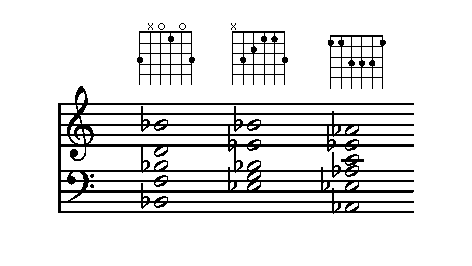
\includegraphics{examples/first-fret-lute-chords.pdf}
\caption{Common chords on the lute using the first fret}
\label{first-fret-lute-chords}
\end{example}

While these figures demonstrate that a lute can be placed in a meantone fretting,
it does not imply that it is a requirement. Composers such as Bottrigari seemed 
to think that the lute was simply an instrument that played in
equal semitones, even in ensembles with instruments that played un-equally.
In the discussion between his two fictional protagonists in \textit{Il Desiderio}, 
Benelli tells Desiderio:

\begin{blocks}
Therefore I do not wish either to affirm or deny, or even to dispute, whether or not 
the semitone said to be minor is minor, or if indeed it has a position between the 
greatest and the least; it will suffice to demonstrate by its effects -- i.e. the
Clavicembalo, the Organ, and their like, sound two unequal semitones, one larger 
than the other. The Lute and the Viols sound two equal semitones, that is, a tone
divided into two equal semitones according to the idea of Aristoxenus. \autocite[17]{HB:1}
\end{blocks}

Bottrigari was comfortable with this arrangement because he classified the instruments into different categories.
According to him, instruments fell into three different types: 1) stable; 2) stable but alterable; and, 3) completely
alterable. The determining factor for an instrument was its ability to alter pitch. Instruments in the first category
were stable because their pitches could not be altered. These included all keyboard instruments. The third category
included instruments whose pitches were entirely changeable, such as the trombone and violin. Their pitches existed
continuously, either along the slide of the trombone, or at any point on the fingerboard of a violin. In the middle,
where instruments are ``stable but alterable'', is where we find lutes, viols, recorders, and transverse flutes. In
Bottrigari's second category of instruments, pitches existed at fixed points but were variable to certain degree. Flute
players could vary pitch by changing the placement of their fingers, or controlling their breath. Lute players,
according to Bottrigari, could ``touch their frets a little higher or a little lower'' in order to vary their pitches.
\autocite[15]{HB:1}

The suggestion here is that lutes played in ensembles using a different temperament than the rest of the instruments.
Keyboard instruments would have used a meantone, or other kind of unequal temperament, and the lutes would have played
with these unequally-tuned instruments using their native quasi-equal temperament. In order for such an ensemble to be
successful, Bottrigari suggests that only the instruments of the first two categories, stable and stable but alterable,
or those from the first and third, stable and entirely alterable, be used together, and never all three together. The
problem with using all three, according to him, is that the middle group will not be able to match pitches with the
first and third groups at the same time. To this, he also adds: ``I think it best to add that no concert of instruments
should ever be given without the addition of a human voice.'' \autocite[23]{HB:1}

For Bottrigari, the issue was not with temperament, but with arrangement and orchestration. Certain instruments should
only play with one kind of instrument and not another. While this provides players some latitude when choosing
temperaments, it still begs the question as to how players could have adjusted their instruments to match other
instruments tuned in a meantone temperament. For that, we should examine a kind of lute that was specifically designed
for ensemble use.

\section{The Theorbo}

As lutes were used more and more in ensembles towards the end of the sixteenth century, a new type of lute was invented
specifically intended to be played in ensembles. The theorbo, as it was called, was a much larger instrument and had
additional bass strings that extended beyond the length of the neck. Although all kinds of lutes, including the theorbo,
were generally fretted in the same way, the tuning of the theorbo presented other alternative fretting solutions that
were not available on lutes using standard tuning. The theorbo's nominal pitch was almost always A, instead of the G as
with other lutes of the time. Technically, any lute or theorbo can be tuned to any key, and it was not uncommon to find
lutes pitched to F, G, A, and D. This applied to lutes in a consort where each instrument existed in a variety of sizes.
The pitch could also result from the instrument's mensur length. The top string would be tuned as high as possible
without breaking and that point determined the overall pitch of the instrument.

In an ensemble, the pitch of a lute or theorbo had to be standardized so that it could play with other instruments. In
English consort music as well as most lute song publications in England, the standard lute pitch was G. In Italy,
however, the theorbo was usually pitched to A. Regardless of the pitch of a lute, it was tuned so that the preceding
course was lower than the one following it. (see example~\ref{g-lute}) This was not the case for the theorbo, which had
first and second courses that were an octave lower. (see example~\ref{a-theorbo})

\begin{example}[h]
\centering
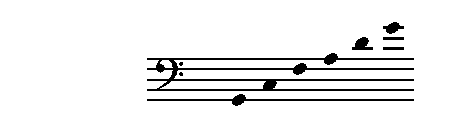
\includegraphics{examples/lute-tuning.pdf}
\caption{Standard lute tuning in G}
\label{g-lute}
\end{example}
\begin{example}[h]
\centering
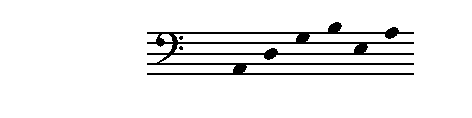
\includegraphics{examples/theorbo-tuning.pdf}
\caption{Theorbo tuned in A with re-entrant first and second courses}
\label{a-theorbo}
\end{example}

Since theorbos were designed for accompaniment and needed to provide more volume than other lutes of the day, the body
size was much larger and the strings longer. Because of the increased mensur length, it was not possible to preserve the
low to high arrangement of courses as they were on the lute. Players found that as they tried to tune the upper strings
to their normal lute pitches, they would break and it was not possible to fashion a gut string thin enough to hold the
pitch at that length. To solve the problem, they tuned the strings to the same pitch but at an octave lower, thus
preserving the same intervalic relationships between strings as they were on the lute. This made chord shapes identical
between instruments and only altered the voicing of the chords. Since the theorbo was primarily a continuo instrument,
the change in voicing did not present a problem; in fact, it became more of an advantage. The re-entrant tuning kept the
overall tessitura of the instrument lower and away from that of the accompanied singer or instrumentalist.

All theorbos had eight additional bass strings that descended diatonically in
pitch from the A on the sixth course. Therefore, the seventh, eighth, and ninth
courses would be G, F, and E, continuing on to an octave G on the fourteenth
course. The disposition of these lower courses varied somewhat from instrument
to instrument. Praetorius discussed two kinds of theorbos: the first he called
a Roman style theorbo, which had six courses on the fretboard; and a second,
which he called the Paduan-style theorbo that had eight courses on the
fretboard. \autocite[59]{MP:1} Because of this variation, players today may
opt to have their seventh and eighth courses on their fretboards before the
additional strings on the extended neck. See figure ~\ref{fig:theorbo-extended}
below.
\begin{figure}[ht]
\centering
\setlength{\unitlength}{0.5mm}
\begin{picture}(80,191.6)
% Draw fingerboard edges
\color{black}
\linethickness{0.075mm}
\put(0,0){\line(0,1){186.6}}
\put(80,0){\line(0,1){186.6}}

% Draw strings
\color{strings}
\linethickness{0.5mm}
\put(5,0){\line(0,1){186.6}}
\put(15,0){\line(0,1){186.6}}
\put(25,0){\line(0,1){186.6}}
\put(35,0){\line(0,1){186.6}}
\put(45,0){\line(0,1){186.6}}
\put(55,0){\line(0,1){186.6}}
\put(65,0){\line(0,1){186.6}}
\put(75,0){\line(0,1){186.6}}

% Insert string pitch names for lute in A (theorbo)

\color{black}
\put(2,191.6){\small{F}}

\put(14,191.6){\small{G}}

\put(24,191.6){\small{A}}

\put(34,191.6){\small{d}}

\put(43,191.6){\small{g}}

\put(53,191.6){\small{b}}
\put(63,191.6){\small{e'}}
\put(73,191.6){\small{a'}}


\color{black}
\linethickness{1mm}
\put(0,136.2){\line(1,0){80}}
\color{black}
\put(80,135.2){\small{\textemdash  1st (diatonic)}}
\color{black}
\linethickness{1mm}
\put(0,107.6){\line(1,0){80}}
\color{black}
\put(80,106.6){\small{\textemdash  2nd (chromatic)}}
\color{black}
\linethickness{1mm}
\put(0,41.3){\line(1,0){80}}
\color{black}
\put(80,40.3){\small{\textemdash  4th (chromatic)}}
\color{black}
\linethickness{1mm}
\put(0,5){\line(1,0){80}}
\color{black}
\put(80,4){\small{\textemdash  5th (diatonic)}}
\color{black}
\linethickness{1mm}
\put(0,66.9){\line(1,0){80}}
\color{black}
\put(80,65.9){\small{\textemdash  3rd (diatonic)}}
\color{black}
\linethickness{1mm}
\put(0,181.6){\line(1,0){80}}
\color{black}
\put(80,180.6){\small{\textemdash  Nut}}
\color{black}
\put(2,158.9){\small{G$\flat$}}
\put(12,158.9){\small{A$\flat$}}
\put(22,158.9){\small{B$\flat$}}
\put(32,158.9){\small{e$\flat$}}
\put(42,158.9){\small{a$\flat$}}
\put(52,158.9){\small{c'}}
\put(62,158.9){\small{f'}}
\put(72,158.9){\small{b$\flat$'}}
\color{black}
\put(22,23.1){\small{d}}
\put(32,23.1){\small{g}}
\put(42,23.1){\small{c'}}
\put(52,23.1){\small{e'}}
\put(62,23.1){\small{a'}}
\put(72,23.1){\small{d''}}
\color{black}
\put(22,87.2){\small{c}}
\put(32,87.2){\small{f}}
\put(42,87.2){\small{b$\flat$}}
\put(52,87.2){\small{d'}}
\put(62,87.2){\small{g'}}
\put(72,87.2){\small{c''}}
\color{black}
\put(22,54.1){\small{c$\sharp$}}
\put(32,54.1){\small{f$\sharp$}}
\put(42,54.1){\small{b}}
\put(52,54.1){\small{d$\sharp$'}}
\put(62,54.1){\small{g$\sharp$'}}
\put(72,54.1){\small{c$\sharp$''}}
\color{black}
\put(22,121.9){\small{B}}
\put(32,121.9){\small{e}}
\put(42,121.9){\small{a}}
\put(52,121.9){\small{c$\sharp$'}}
\put(62,121.9){\small{f$\sharp$'}}
\put(72,121.9){\small{b}'}
\end{picture}
\caption{Theorbo with extend courses}
\label{fig:theorbo-extended}
\end{figure}

The advantage to having these additional courses on the neck is that a player is
able to fret additional chromatic notes with the left hand. On the longer
strings that are attached to the extension this is not possible and any
chromatic changes in the pitches of those strings must be done using the tuning
pegs prior to playing.

While it might have been possible to tune a lute's first course to a chromatic semitone, this was impossible on the
theorbo. For example, the first fret had to be diatonic because of the open E$\natural$ and B$\natural$ on the second
and third courses so that the pitches on those courses on the first fret would be F$\natural$ and C$\natural$. If a
chromatic semitone was used, an E$\sharp$ and B$\sharp$ would result, making this type of semitone unusable. Similarly,
the presence of a B$\flat$ at the third fret of the fourth course dictates that the next fret must be chromatic to
create a B$\natural$ at the fourth fret of the same course. Even the sixth fret is determined to be diatonic because of
the E$\natural$ to F$\natural$ that occurs on the third course. These restrictions could explain why Praetorius's
theorbo had all of its extended courses on the long neck, and off of the fretted short neck. This would enable the
player to set a fixed F$\sharp$ and G$\sharp$ on the seventh and eight courses and leave the pitches on the first fret
in their preferred diatonic semitones.

Essentially, the frets of a theorbo tuned to meantone temperament were ``fixed'' in their positions because the location
of the diatonic semitones between B and C, and E and F, determined whether the fret was either chromatic or diatonic. If
we also take into consideration the similar issue of octaves affecting the position of frets on the lute in G, it is
apparent that a theorbo should have its initial five frets arranged the same way as a lute, with a diatonic semitone for
the first fret and alternating diatonic and chromatic semitones for successive frets. If we was to blend successfully
with quarter-comma meantone, we will need to limit some of the semitones that are available on our instruments and find
alternative methods of playing them.

\subsection{Solutions Utilizing Re-entrant Tuning}

The theorbo has the advantage of using both chromatic and diatonic semitones within the same octave. Because of the re-
entrant nature of the theorbo's tuning, certain notes that are an octave apart on the lute are unisons on a theorbo.
This offers a possible solution to some of the problems of semitone size because a particular pitch could be a diatonic
semitone at one fret while being chromatic at a different fret, and still be in the same octave. Referring to
figure~\ref{fig:theorbo-extended}, the A$\flat$ on the first fret of the fourth course and the G$\sharp$ found on the
fourth fret of the second course are in the same octave, whereas on a lute in standard G tuning they are an octave
apart. Other notes are still an octave apart, such as the E$\flat$ on the fifth course of the first fret and the
D$\sharp$ on the third course of the fourth fret. However, in continuo playing octave displacement does not matter and
players are able to substitute different octaves as needed. Therefore, all the player has to do is choose the
appropriate fingering for the left hand to obtain either the chromatic or diatonic semitone.

For chords that require chromatic semitones, such as a G$\sharp$ or a D$\sharp$, the
player can use pitches found on the fourth fret. Some of the more common left-hand chord
patterns that use this fret include the E major triad and chords with a
sixth above the bass.
\begin{example}[h]
\centering
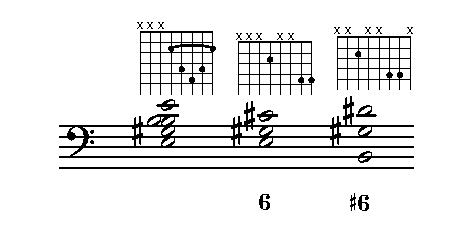
\includegraphics{examples/g-sharp.pdf}
\caption{Chords using chromatic semitones on the fourth fret}
\label{fourth-fret-chords}
\end{example}
For others requiring diatonic semitones, such as the A$\flat$ or E$\flat$, the
player may use pitches on the first fret. These include A$\flat$ major, F minor, and C
minor.
\begin{example}[h]
\centering
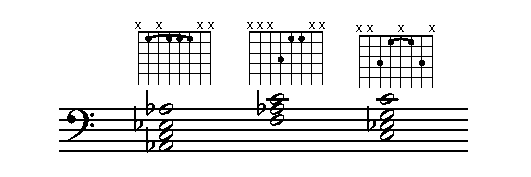
\includegraphics{examples/a-flat.pdf}
\caption{Chords using diatonic semitones on the first fret}
\label{first-fret-chords}
\end{example}
Although instances of an A$\flat$ major triad are rare, all the needed pitches are on
the first fret, and F minor and C minor triads are both possible using a limited
number of voices.

While re-entrant tuning makes it possible to play chords with different kinds of
semitones, sometimes the left-hand chord fingerings that result are not the easiest to
execute, nor are they as idiomatic to the instrument as other more commonly used
fingerings. More ideal chords for the theorbo are easier to execute, have more potential
voices, and favor open strings whenever possible. The fingerings for F
minor and C minor listed in example~\ref{first-fret-chords} are not commonly found in
existing theorbo tablatures of the time, nor are they used very often among modern
players. The more common fingerings for these chords use the fourth fret.
Additionally, the E major chord in example~\ref{fourth-fret-chords} uses the chromatic
semitone on the fourth fret, but ignores the open E and B on the third and second
courses. More common chord fingerings below in example~\ref{common-chords} indicate that
a player would more likely use a fully-voiced F minor or C minor chord with a barre at
the third fret than those listed previously. An E major chord that makes use of the
open B and E strings sounds much more resonant and is easier for the left hand.
\begin{example}[h]
\centering
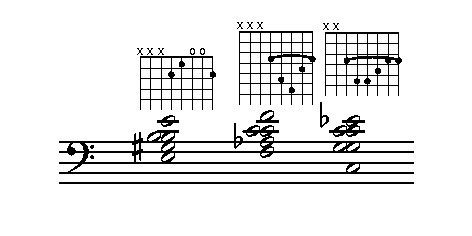
\includegraphics{examples/common-chords.pdf}
\caption{Common theorbo chord shapes}
\label{common-chords}
\end{example}
The obvious problem with these more idiomatic chord shapes is that if they are used on
a theorbo in meantone temperament, their semitones are the opposite of what they should be.
The E major chord shown above would have a diatonic A$\flat$ instead of the chromatic
G$\sharp$ and the thirds of the F minor and C minor chords would be chromatic in nature
instead of diatonic.

The question raised here is: how did players manage in a meantone temperament
without the use of their common chord patterns? In a small ensemble, without
keyboards or other instruments with meantone requirements, we might have the
option of using a non-meantone temperament; however, if this is not desirable,
we should look at other available modifications to make meantone more successful
on our instruments. Selective left-hand fingerings alone are not enough to overcome
the problems imposed by meantone temperaments.

\subsection{Tastini}

The advantages that re-entrant tuning offers can render more idiomatic chord shapes unusable in a meantone temperament.
If we are to use these shapes, yet still be able to play in meantone, we need the ability to apply different semitones
locally within a fret instead of being forced to have all the pitches at one fret of a certain size. In other words, we
need to mix both chromatic and diatonic semitone sizes within the same fret. For example, consider the pitches of the
extended bass courses: the first chromatic note on the seventh and eighth courses is determined by the quality of the
first fret. Since the first fret on a theorbo is a diatonic semitone, this would make the pitches on this fret for these
two lower courses A$\flat$ and G$\flat$, respectively. It is far more likely that a G$\sharp$ and an F$\sharp$ are
needed, but shifting the entire first fret to a chromatic semitone would alter the rest of the notes and result in a
B$\sharp$ on the third course instead of a C.

To correct this problem and apply a chromatic semitone localized only to one or two courses, lute players during this
time employed the use of \textit{tastini}. The diminutive form of \textit{tasto}, the Italian word for fret, these
``little frets'' were small pieces of wood that were glued to the fretboard to create a chromatic semitone on one or two
courses while the remainder of the courses on the fret were diatonic. Courses beyond the sixth on a theorbo were used
for bass support, and any that were on the fretboard, such as the seventh and eighth course, were only stopped at the
first fret. This made the use of tastini an ideal choice since it only affected the first fret. Players now had the
ability to use an F$\sharp$ and G$\sharp$ while keeping the rest of the pitches on the first fret at their original
diatonic position. See figure~\ref{fig:theorbo-tastini}.

\begin{figure}[ht]
\centering
\setlength{\unitlength}{0.5mm}
\begin{picture}(80,191.6)
% Draw fingerboard edges
\color{black}
\linethickness{0.075mm}
\put(0,0){\line(0,1){186.6}}
\put(80,0){\line(0,1){186.6}}

% Draw strings
\color{strings}
\linethickness{0.5mm}
\put(5,0){\line(0,1){186.6}}
\put(15,0){\line(0,1){186.6}}
\put(25,0){\line(0,1){186.6}}
\put(35,0){\line(0,1){186.6}}
\put(45,0){\line(0,1){186.6}}
\put(55,0){\line(0,1){186.6}}
\put(65,0){\line(0,1){186.6}}
\put(75,0){\line(0,1){186.6}}

% Insert string pitch names for lute in A (theorbo)

\color{black}
\put(2,191.6){\small{F}}

\put(14,191.6){\small{G}}

\put(24,191.6){\small{A}}

\put(34,191.6){\small{d}}

\put(43,191.6){\small{g}}

\put(53,191.6){\small{b}}
\put(63,191.6){\small{e'}}
\put(73,191.6){\small{a'}}


\color{black}
\linethickness{1mm}
\put(0,136.2){\line(1,0){80}}
% tastini at 7 and 8 (first fret)
\put(2,151){\line(1,0){17}}
% tastino at 4 (first fret)
\put(42,151){\line(1,0){8.5}}
% tastino at 3 (above fourth fret)
%\put(52,23.1){\line(1,0){8.5}}
\color{black}
\put(80,135.2){\small{\textemdash  1st (diatonic)}}
\color{black}
\linethickness{1mm}
\put(0,107.6){\line(1,0){80}}
\color{black}
\put(80,106.6){\small{\textemdash  2nd (chromatic)}}
\color{black}
\linethickness{1mm}
\put(0,41.3){\line(1,0){80}}
\color{black}
\put(80,40.3){\small{\textemdash  4th (chromatic)}}
\color{black}
\linethickness{1mm}
\put(0,5){\line(1,0){80}}
\color{black}
\put(80,4){\small{\textemdash  5th (diatonic)}}
\color{black}
\linethickness{1mm}
\put(0,66.9){\line(1,0){80}}
\color{black}
\put(80,65.9){\small{\textemdash  3rd (diatonic)}}
\color{black}
\linethickness{1mm}
\put(0,181.6){\line(1,0){80}}
\color{black}
\put(80,180.6){\small{\textemdash  Nut}}
\color{black}
\put(2,158.9){\small{F$\sharp$}}
\put(12,158.9){\small{G$\sharp$}}
\put(22,158.9){\small{B$\flat$}}
\put(32,158.9){\small{e$\flat$}}
\put(42,158.9){\small{g$\sharp$}}
\put(52,158.9){\small{c'}}
\put(62,158.9){\small{f'}}
\put(72,158.9){\small{b$\flat$'}}
\color{black}
% Tastini pitches on first fret
\put(2,140){\small{G$\flat$}}
\put(12,140){\small{A$\flat$}}
\put(42,140){\small{a$\flat$}}
% Tastini pitch below the fifth
%\put(52,30){\small{E$\flat$}}
\put(22,13.1){\small{d}}
\put(32,13.1){\small{g}}
\put(42,13.1){\small{c'}}
\put(52,13.1){\small{e'}}
\put(62,13.1){\small{a'}}
\put(72,13.1){\small{d''}}
\color{black}
\put(22,87.2){\small{c}}
\put(32,87.2){\small{f}}
\put(42,87.2){\small{b$\flat$}}
\put(52,87.2){\small{d'}}
\put(62,87.2){\small{g'}}
\put(72,87.2){\small{c''}}
\color{black}
\put(22,54.1){\small{c$\sharp$}}
\put(32,54.1){\small{f$\sharp$}}
\put(42,54.1){\small{b}}
\put(52,54.1){\small{d$\sharp$'}}
\put(62,54.1){\small{g$\sharp$'}}
\put(72,54.1){\small{c$\sharp$''}}
\color{black}
\put(22,121.9){\small{B}}
\put(32,121.9){\small{e}}
\put(42,121.9){\small{a}}
\put(52,121.9){\small{c$\sharp$'}}
\put(62,121.9){\small{f$\sharp$'}}
\put(72,121.9){\small{b'}}
\end{picture}
\caption{Theorbo with added tastini}
\label{fig:theorbo-tastini}
\end{figure}


Players today have employed tastini on other frets as well, which can help solve the previous problems of idiomatic
chord shapes in meantone frettings. Referring again to figure~\ref{fig:theorbo-tastini}, an additional tastino on the
fourth course can provide us with a G$\sharp$, which enables us to play the more common E major chord shape described in
example~\ref{common-chords} using the open strings on courses two and three. The problem of C minor and F minor chords,
however, still remains. We could switch the entire fourth fret to a diatonic semitone, thereby giving us the needed
pitches, but we would lose the ability to play some of the sixth chords described in example~\ref{fourth-fret-chords}.
One could argue that additional tastini at the fourth fret could correct this problem, but such a solution might become
unwieldy. Also, it means sacrificing several chromatic semitones, in this case C$\sharp$, F$\sharp$ and G$\sharp$, for
the sake of two diatonic ones: E$\flat$ and A$\flat$.

While modern players have embraced the use of tastini, there are no surviving instruments with their tastini intact.
Yet, it is obvious they were in use because of the different historical accounts that describe them. The earliest of
these comes from Vicenzo Galilei's \textit{Fronimo}, where he did not have very good things to say about them. Galilei's
description of tastini suggests that players were using them in different places on the instrument and not just the
first fret.\autocite[165]{VG:1} Today, tastini are found usually only on theorbos, almost always at the first fret, and
rarely elsewhere. There are exceptions to this, and players today are free to put tastini anywhere, but the most common
location seems to be at the first fret.

Galilei's main disagreement over the use of tastini was that it made adjustments to one fret only in a certain pitch
context, for example when F$\sharp$ is wanted instead of a G$\flat$, but that one adjustment does not work in other
pitch contexts or match the same pitch at a different location on the fingerboard. He also maintained that the lute was
tuned in equal semitones and that a well-placed fretting system was sufficient to play all the pitches necessary. In his
mind, tastini ruined that sort of system because if the lute were tuned in equal semitones, there would be no need for a
tastino: the fret would function correctly as either a chromatic or diatonic semitone.

Whether or not we follow Galilei's advice, his attitude towards tastini is the most important indicator that they were
in use. Some players must have used them at this time, otherwise Galilei would not have mentioned it. However, we must
note that the manner in which Galilei describes their usage appears to have no direct application to correcting the
problems found in quarter-comma meantone. After all, since Galilei tuned equally, meantone was not an issue for him. All
of this points to the fact that if we are to use tastini on our theorbo or lute, it must be in a way Galilei had not
envisioned, and so we are left to create our own solutions.

Bermudo has a brief account of tastini in the context of the vihuela. His description
of their use fits very closely with our current usage of them:
\begin{blocks}
For faults that may arise, take the advice given before of looking for the notes on other
frets, or with the pressure of the finger when stopping the note, of by placing another
fret in front of the principle fret, which, when placed for this purpose, should be
thicker than the first fret so that it does not rub against the string. This [extra]
fret can be placed by dividing the distance from the third fret to the bridge into eight
parts, and wherever the compass reaches [downward from the third fret] will be the first
fret, which will form \textit{fa}. \autocite[115-116]{DE:1}
\end{blocks}
Recalling table~\ref{table:comparison}, Bermudo's first fret is a diatonic semitone or what
he calls \textit{fa}. In order to obtain the chromatic fret, or \text{mi}, Bermudo
proposes an additional fret that is front of the first fret, or placed between the nut
and the first fret. He says the fret should be slightly thicker, which we can infer
is so that the \textit{fa} fret does not prevent it from working properly.
\begin{figure}[ht]
\centering
\setlength{\unitlength}{1mm}
\begin{picture}(60,87.8)
% Draw fingerboard edges
\color{black}
\linethickness{0.075mm}
\put(0,0){\line(0,1){87.8}}
\put(60,0){\line(0,1){87.8}}

% Draw strings
% 6th course
\color{strings}
\linethickness{0.5mm}
\put(5,0){\line(0,1){87.8}}
\linethickness{0.25mm}
\put(7,0){\line(0,1){87.8}}
% 5th course
\put(15,0){\line(0,1){87.8}}
\put(17,0){\line(0,1){87.8}}
% 4th course
\put(25,0){\line(0,1){87.8}}
\put(27,0){\line(0,1){87.8}}
% 3rd course
\put(35,0){\line(0,1){87.8}}
\put(37,0){\line(0,1){87.8}}
% 2nd course
\put(45,0){\line(0,1){87.8}}
\put(47,0){\line(0,1){87.8}}
% 1st course
\put(56,0){\line(0,1){87.8}}
\color{black}
\linethickness{1mm}
\put(0,38.3){\line(1,0){60}}
\color{black}
\put(60,37.3){\small{\textemdash  fa}}
\color{black}
\linethickness{1mm}
\put(0,48.4){\line(1,0){60}}
\color{black}
\put(60,47.4){\small{\textemdash mi}}
\color{black}
\linethickness{1mm}
\put(0,5){\line(1,0){60}}
\color{black}
\put(60,4){\small{\textemdash 2nd fret}}
\color{black}
\linethickness{1mm}
\put(0,82.8){\line(1,0){60}}
\color{black}
\put(60,81.8){\small{\textemdash  Nut}}
\end{picture}
\caption{Bermudo's \textit{mi} and \textit{fa} first frets}
\label{fig:bermudo-1-mifa}
\end{figure}

Although these are not true tastini, insofar as his fret spans the entire
fingerboard instead of just the affected course, it is the strongest evidence we have
in support of using any kind of additional fret to create both chromatic and diatonic semitones.

A later reference to tastini from the seventeenth-century comes from Jean Denis who
was a harpsichord builder during the first half of the the century. He refers to
``staggered'' frets on the lute which could be made of ivory. The reference appears in
Lindley's book, and the context in which Denis was discussing tastini was that
someone had tuned a harpsichord in equal temperament. Denis criticizes this approach
stating that someone should perfect the lute and viola da gamba so that they may
accommodate unequal semitones instead of ``ruining a good and perfect tuning in order to
accommodate imperfect instruments.''\autocite[47]{ML:1}.

Another reference comes from Christopher Simpson's \textit{A Compendium of Practical
Music} and appears to describe tastini as they are commonly used today on the theorbo:
\begin{blocks}
I do not deny but that the slitting [\textit{sic}] of the keys in harpsichords and organs, as also the
placing of a middle fret near the top or nut of the viol or theorbo where the space is
wide, may be useful in some cases for the sweetening of such dissonances as may happen
in those places; but I do not conceive that the enharmonic scale is therein concerned,
seeing those dissonances are sometimes more, sometimes less, and seldom that any of them
do hit precisely the quarter of a note. \autocite[51]{CS:1}
\end{blocks}
The first part of Simpson's description matches Bermudo's additional fret exactly, as he describes
an additional fret between the first fret and the nut. He does not state whether or not this middle
fret spans the entire fretboard. The second part of his statement refers to the difference between
the diatonic and chromatic semitone. Simpson calls these ``quarter notes'' as we today might refer
to quarter tones, or half of a semitone. He seems to think that, from a practical standpoint, these
semitones are seldom precisely what they are supposed to be, either diatonic or chromatic. Simpson's
opinions aside, he does provide us with evidence that tastini or additional frets were used
historically in the same places on the fretboard of a lute as players might use them now. Beyond
tastini, there are more possibilities to overcome some of the difficult issues pertaining to
quarter-comma meantone temperament and frets.

\subsection{Other Solutions}

Aside from tastini, there were diverse methods by which lutenists were able to
coax meantone temperaments from their fretting. One of these involved placing frets at
an angle so that a fret could be diatonic on one side of the fingerboard and chromatic on
the other. For the theorbo, this could be used as a substitute for tastini. It
is possible to use an angled first fret, for example, to achieve the chromatic
semitones necessary on the seventh and eighth courses. Instead of placing a tastino at
the left side of the fingerboard, the first fret could be slanted so that it
angled towards the chromatic side of the semitone as it moved towards the
lower courses.

The problem with this is that pitches in the middle of the fret are somewhere between
chromatic and diatonic. Juan Bermudo discusses the practice of angled frets on the
vihuela and comes to the same conclusions:
\begin{blocks}
[...] some players hope to fix the abovementioned faults by putting the frets where the
said faults occur at an angle, taking them out of line. This is not a solution but a
cover-up [...] Take a fret where there is a fault (where it is \textit{mi} for strings
but needs to be \textit{fa} for others) and you will find that, by slanting the fret,
it does not hit any string in the right place. \autocite[112-113]{DE:1}
\end{blocks}
While we might be able to achieve a chromatic semitone at the eighth course, each
successive course would be slightly sharper until reaching the top course. Only the
first and last courses would be truly either chromatic or diatonic, the courses in the
middle would be something in between and not in a specific temperament.

Despite what Bermudo and other writers of the time have said about angled frets, we can
find use for them. Angled frets work best when they are strategically located and used
for frets that might have only one or two useful pitches on them. In a ``standard''
quarter-comma meantone fretting system, as shown in
figure~\ref{fig:quarter-diatonic-complete-a} of the appendix, the sixth fret is diatonic
and duplicates the E$\flat$ and A$\flat$ found at the first fret. A common left-hand
fingering for the first inversion triad, or a chord with a \textit{6} above the bass,
uses the bass on the fifth and sixth courses. These include the first-inversion D major
triad with the F$\sharp$ as well as the first-inversion A major triad with the
C$\sharp$, both found on the fourth fret. However, we lack the G$\sharp$ or D$\sharp$
for either E major or B major tonalities. If we move our sixth fret, which is commonly
diatonic, so that it is placed at an angle, it is possible to get a very close
approximation of a chromatic semitone for these pitches (see
figure~\ref{theorbo-slanted-sixth}). The slanted sixth fret allows us to play the
needed triads with G$\sharp$ and D$\sharp$ in the bass, and disadvantages are minimized
because the sixth fret is not commonly used in other left-hand chord shapes.
\begin{figure}[ht]
\centering
\setlength{\unitlength}{0.5mm}
\begin{picture}(80,70)
% Draw fingerboard edges
\color{black}
\linethickness{0.075mm}
\put(0,0){\line(0,1){70}}
\put(80,0){\line(0,1){70}}

% Draw strings
\color{strings}
\linethickness{0.5mm}
\put(5,0){\line(0,1){70}}
\put(15,0){\line(0,1){70}}
\put(25,0){\line(0,1){70}}
\put(35,0){\line(0,1){70}}
\put(45,0){\line(0,1){70}}
\put(55,0){\line(0,1){70}}
\put(65,0){\line(0,1){70}}
\put(75,0){\line(0,1){70}}

% Fifth course pitch names
\color{black}
\put(24,70){\small{d}}
\put(34,70){\small{g}}
\put(43,70){\small{c''}}
\put(53,70){\small{e''}}
\put(63,70){\small{a''}}
\put(73,70){\small{d''}}

\color{black}
\thicklines
\put(80,26.4){\line(-6,1){80}}
\color{black}
\put(80,25.4){\small{\textemdash  6th (diatonic)}}
\color{black}
\linethickness{1mm}
\put(0,5){\line(1,0){80}}
\color{black}
\put(80,4){\small{\textemdash  7th (chromatic)}}
\color{black}
\linethickness{1mm}
\put(0,60.3){\line(1,0){80}}
\color{black}
\put(80,59.3){\small{\textemdash  5th (diatonic)}}
\color{black}
\put(22,43.3){\small{f$\sharp$}}
\put(32,43.3){\small{g$\sharp$}?}
\put(42,43.3){\small{d$\flat$'}}
\put(52,43.3){\small{f'}}
\put(62,43.3){\small{b$\flat$'}}
\put(72,43.3){\small{e$\flat$''}}
\color{black}
\put(22,15.7){\small{e}}
\put(32,15.7){\small{a}}
\put(42,15.7){\small{d'}}
\put(52,15.7){\small{f$\sharp$'}}
\put(62,15.7){\small{b'}}
\put(72,15.7){\small{e''}}
\end{picture}
\caption{Theorbo with angled sixth fret}
\label{fig:theorbo-slanted-sixth}
\end{figure}

Alternatively, we could employ a tastino underneath these two courses and avoid the
slanted fret altogether; however, such a solution would be at the player's discretion.

Other solutions for achieving a successful quarter-comma meantone temperament do not involve
adjusting frets at all, and advocate positioning the left hand so that individual courses are pulled in
one direction or another to raise their pitch slightly and compensate for frets that are using an
incorrect semitone. Praetorius describes such a method in his \textit{Syntagma Musicum}:
\begin{blocks}
Thus the semitones cannot be either major nor minor, but are, perforce, ``intermediate''
if anything. For I reckon that each fret [...] contains four-and-a-half commas, whereas
the major semitone contains five and the minor semitone only four. Since the error is
only half a comma either way, the ear hardly notices it with these instruments [...]
Major and minor semitones are both produced by the same fret, both sound in tune, [...]
especially since by particular applications of the finger to the string, over the fret,
it is possible to have some control over the pitch of the note produced.
\autocite[68]{MP:1}
\end{blocks}
It is clear that Praetorius is describing meantone temperament, because he
refers to chromatic (minor) and diatonic (major) semitones as having different numbers of
commas. However, Praetorius is actually referring to sixth-comma temperament
which divides its wholetones into nine commas, split four to five, versus a quarter-comma
which contains five commas per wholetone and is divided two to three.

\textit{Syntagma} was published in 1619, so we might assume that sixth-comma meantone had begun to replace quarter-comma
in some musical circles, but it is still a meantone temperament. More importantly, Praetorius describes fretted
instruments as having equal semitones, divided exactly in the middle between chromatic and diatonic, but essentially
played unequally. According to him, the player has the ability to change the quality of the semitones so that they might
be close to chromatic or diatonic as the music requires.

Additional evidence of using finger pressure to correct pitch problems is found in Bermudo's treatise. He advises
players either to locate the note somewhere else on the fingerboard or to use finger pressure to alter it, and refers to
this method several times in his treatise, indicating that it might have been preferable to the addition of extra frets.
\autocite[106]{DE:1} Bottrigari also describes this same technique, when he says players ``touch their frets a little
higher or a little lower'', as I mentioned earlier. \autocite[15]{HB:1}

Bending pitches using variable pressure in the left-hand, such as Praetorius, Bermudo, and Bottrigari describe, is
possible, but not easily done. Another common way for a lutenist to bend pitches is to pull the course with the finger
to one side or the other. This technique is very common in twentieth-century classical guitar literature where extreme
fluctuations of pitch are exploited for various compositional reasons. Although there is no evidence of its use in
historical lute tablatures or other musical sources for lute or theorbo, it is possible to conjecture that players
during that time might have found a way to utilize it in one form or another in order to adjust to meantone in ensemble
playing.

\section{Meantone Fretting in Tablature Sources}

Thus far, we have discussed the methods by which lute players can adapt to the problems of quarter-comma meantone
fretting systems in ensemble situations. For the most part, these methods require the player to place certain notes on
certain frets. In ensemble music, where basso continuo is used, the player has the ability to do this because the music
is in staff notation and no left-hand pitches are dictated anywhere. In fact, it is customary for players to move bass
notes into different octaves when necessary and even use reduction methods that omit repetitive notes. In essence, the
player may re-compose sections of his or her part to fit the instrument's compass and make it sound as idiomatic as
possible.

In lute tablature sources, the placement of notes in the left-hand is precisely dictated. The player usually does not
move notes to different locations on the fretboard in order to compensate for any potentially incorrect semitones in a
meantone temperament. Because of this fact, tablature sources alone indicate that quarter-comma meantone temperament is
not a viable temperament for solo lute literature in the late sixteenth and early seventeenth centuries. Additionally,
ensemble music for lute and voice, where the lute is an accompanying instrument using tablature rather than basso
continuo notation, further indicates that quarter-comma meantone is not usable, and a different kind of temperament
would be preferable, such as sixth-comma meantone or another temperament specific to the lute.

The lute song repertory is a unique genre featuring a lute part written in tablature, one or more
voices, and sometimes a bowed bass. Just as with solo music, players usually do not take the same
liberties with pitch placement as they do when playing basso continuo. In 1597, John Dowland published the
first book of music written in this new genre. Entitled \textit{The First Booke of Songs or Ayres},
his accompaniments were very complete, and equal in caliber to his solo works for lute. The songs
were composed in keys idiomatic for the lute in Renaissance tuning, such as G minor or major. Near the
end of Dowland's first book of Ayres is a well-known song entitled ``Come heavy sleep'' that opens
in G major but has a very striking key change to B major about mid-way through the song at measure 9.
Such a change of tonality befits the subject matter of the song, but if we look closely at
Dowland's placement of the pitches on the lute, they are at odds with a quarter-comma fretting
system.
\begin{example}[h]
\centering
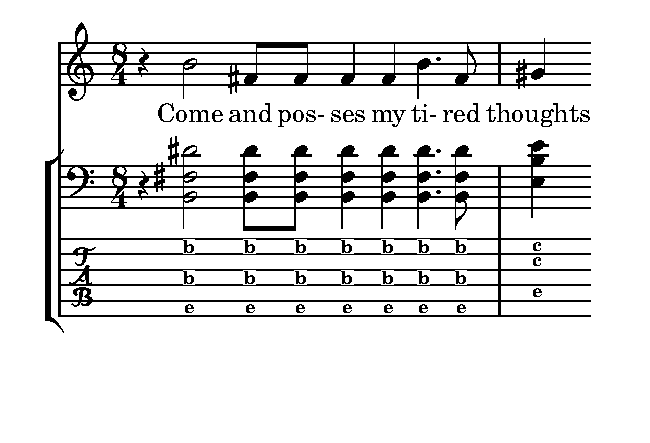
\includegraphics[trim=0 0.5in 0 0,clip=true]{examples/come.pdf}
\caption{Dowland, ``Come heavy sleep'' from \textit{The First Booke of Songs or Ayres} (1597), m. 14}
\label{dowland-come}
\end{example}
In example~\ref{dowland-come}, there are repeated instances of F$\sharp$ and D$\sharp$ in the
first measure of our example, which are represented in the tablature part by the character
\textit{b}. English lute music was written in the French system of tablature, so the
frets are indicated with letters. The tablature character \textit{a} is the open
string and the character \textit{b} is the first fret. If we were trying to follow the
meantone fretting system I outlined earlier, these notes would be G$\flat$ and E$\flat$,
and would sound quite strident against the B. Recalling Dowland's own choice for the
first fret, as shown in table~\ref{table:comparison}, the quality of semitone is diatonic,
but is in sixth-comma and not quarter-comma. A sixth-comma fret would certainly be more
palatable in this case and perhaps explains why Dowland himself was advocating a sixth-comma
diatonic semitone instead of a quarter-comma one.

Other examples from Dowland's works highlight the central problem with employing meantone fretting
systems on lutes. Because of the way in which fretted instruments are tuned, there are cases when
both the diatonic and chromatic semitone are required at the same fret. For example, in his song
\textit{Sorrow stay}, there are both G minor chords and D major chords, which require a
B$\flat$ and an F$\sharp$. However, looking at an excerpt from the song below, we can see that
these notes are both placed on the same fret.
\begin{example}[h]
\centering
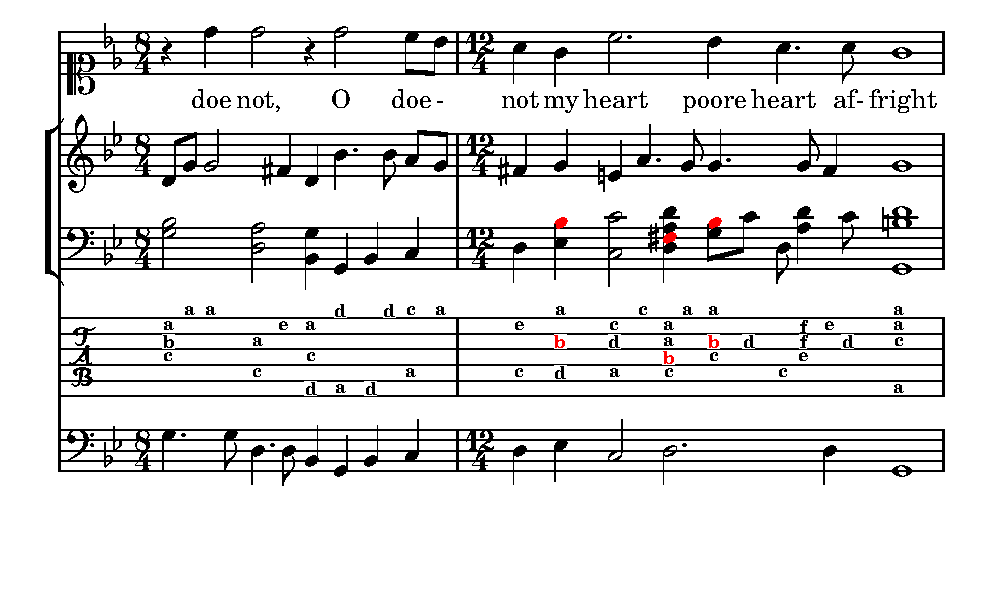
\includegraphics[trim=0in 0.75in 0in 0in,clip=true,width=\textwidth]{examples/saw.pdf}
\label{dowland-saw}
\caption{Dowland, ``Sorrow stay'' from \textit{The Second Booke of Songs or Ayres} (1600), mm. 9--10}
\end{example}
The notes and their corresponding tablature characters are highlighted in red. Both
notes occur on the first fret, where there is the tablature character \textit{b}. If
we were to use a meantone fretting system, the B$\flat$ would be true but the F$\sharp$
would be a G$\flat$ instead, unless we were using a tastino to correct the problem.
This kind of issue results when frets determine the quality of the semitone regardless
of what the particular pitch might be. Keyboard and other instruments are exempt from
this kind of issue because their semitones can be tuned independent of one another. A
keyboard or organ can very easily have F$\sharp$ and B$\flat$ existing at the same time.

Referring back to Dowland's own fretting instructions from the previous chapter, he described one kind of fretting
system that remained fixed once it was set. While he seems to use a sixth-comma diatonic semitone at the first fret,
which would ease the problem of having the F$\sharp$ and B$\flat$ on the same fret, he does not mention the use of
tastini or any other corrective frets. Although it would not sound quite as pronounced as in quarter-comma, the
difference between G$\flat$ and F$\sharp$ would still remain, even in sixth-comma meantone. Since other composers and
lute players were subject to the same tuning constraints, it seems Dowland was trying to create his own temperament that
satisfied both semitone requirements in his works. How he managed to do this is still somewhat of a mystery, since his
own fretting instructions are problematic. His contemporaries might have opted for an equal semitone approach by
splitting the difference between frets or opting for positions that simply satisfied their ears. Yet, the ensemble
dilemma would have remained, and applying an equal semitone solution, a sixth-comma meantone solution, or a completely
original system of fretting, would mean that the lute would be attempting to play in tune with an ensemble that was
using a different temperament.

The same issues that affect fretting systems for Renaissance lute also affect the theorbo as well. Although they are
less common, there are tablature accompaniments for the theorbo, and just as we studied lute tablatures for clues
regarding choices of temperament, we can examine theorbo accompaniment tablatures for the same information. An example
of an early seventeenth-century accompaniment comes from Girolamo Kapsberger, a theorbo player and composer who was
active in Rome. In addition to publishing several books of music for solo theorbo, he published four books of villanelle
written for one, two, and three voices, with written accompaniment for guitar and theorbo. Additional instruments could
have been used, doubling the vocal parts, but Kaspberger is non-specific as to which kinds. The vocal and bass parts are
written in staff notation, while the guitar and theorbo parts are written in their own specialized notation. In the case
of the guitar, alphabetic notation is used, where a series of different letters indicate which chord to play. The
theorbo part is in Italian tablature, where numbers are used in place of letters to indicate fret placement and the
order of strings is actually inverted from French tablature, placing the top string of the theorbo on the bottom line of
the tablature staff. For the sake of consistency, I have transcribed Kapsberger's tablature part into French tablature
so we can compare the examples with lute and theorbo.

The song ``All' ombra'', from his first book of villanelle, contains a cadence in A major
towards the end of the piece. The G$\sharp$ and C that are used are highlighted in red.
\begin{example}[h]
\centering
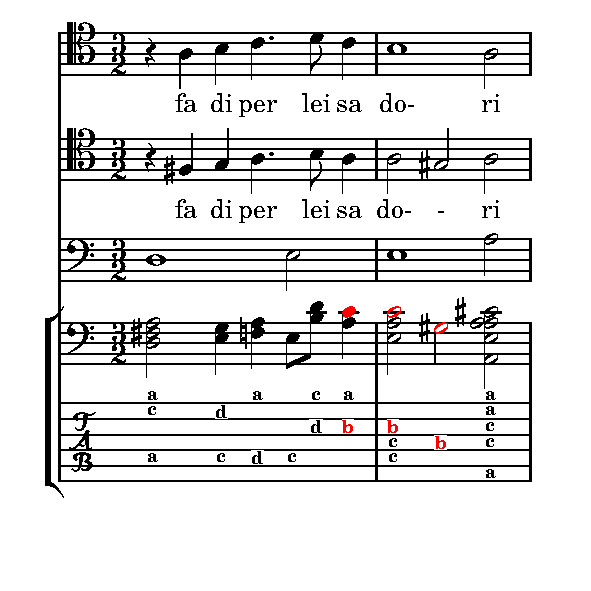
\includegraphics[trim=0 0.5in 0 0,clip=true]{examples/kaps_ombria.pdf}
\label{kaps-ombria}
\caption{Kapsberger, ``All' ombra'' from \textit{Di Villanelle, bk. 1} (16??), mm. 21--22 }
\end{example}
Similar to our previous example from Dowland, these two notes are found on the
same fret, indicated with the tablature character \text{b} highlighted in red.
If we were employing quarter-comma meantone on our theorbo, the G$\sharp$ would
instead be an A$\flat$. If this indeed was the case, this difference in semitone
quality could simply have been accepted. On the other hand, it seems more
likely that an alternative temperament was chosen that would have made the
G$\sharp$ more usable.

If Kapsberger's theorbo was definitely in quarter-comma meantone, a tastino would have been the only solution to avoid
the A$\flat$ issue on his first fret. An alternative solution that I proposed earlier would be to change the left-hand
fingering of the E major chord so that the G$\sharp$ on the fourth fret is used resulting in a chromatic semitone and
not a diatonic one. However, Kapsberger's tablature clearly indicates that the G$\sharp$ on the first fret is to be
used.

While these examples represent only a fraction of the types of problems that lute players faced when tuning to meantone
temperaments, the issue of chromatic versus diatonic frets was so pervasive in the literature that it was impossible to
ignore. According to historical evidence, some of the techniques lute players employed in their attempts to address the
conundrum were controversial. When we are playing in meantone temperaments today, we must be willing to do the same and
apply our own solutions, controversial or otherwise. In the concluding chapter of this study, I will summarize all of
the findings presented here and how we might apply them in today's performances.

\chapter{Solutions for Modern Lutenists}

Given the evidence presented here from historical sources and contemporary sources such
as Mark Lindley's book on historical temperaments for fretted instruments, there are
two clear points that emerge.  First, while most other instruments exclusively used meantone and
temperaments with semitones of varied sizes, lutes also used temperaments with equal
semitones.  This does not imply that they used our modern-day equal temperament, nor
does it imply that they their kind of equal temperament was used exclusively in the same
way that other instruments used non-equal temperaments.  What the evidence shows us is
that lute players had more options when it came to temperaments and that they could take
advantage of these options when it suited their needs.  The second important point
regarding lute temperaments is an indication of how temperaments were viewed as whole.

The nature of lute temperaments as this time indicates that they were not universally
applied in the same way as today's temperaments.  The modern musical world relies on
established standards of pitch as well as temperament.  Such standards did not exist
before the eighteenth century.  Pitch varied from city to city, and even from ensemble
to ensemble.  It seems that the same variation applied to temperaments as well.  A
further distinction is that not only could temperament vary from ensemble to
ensemble, it also might vary between instruments in the same ensemble.

% Examples:
%  - L'Orfeo, Act 5: different tunings, lute in A and lute in G
%  - solo music could have used a different temperament
%  -
%
%
%
%
%
%

% Back matter
\appendix

\chapter{Complete Fretting Diagrams}

\begin{figure}[ht]
\centering
\setlength{\unitlength}{0.5mm}
\begin{picture}(60,365)
% Draw fingerboard edges
\color{black}
\linethickness{0.075mm}
\put(0,0){\line(0,1){360}}
\put(60,0){\line(0,1){360}}

% Draw strings
% 6th course
\color{strings}
\linethickness{0.5mm}
\put(5,0){\line(0,1){360}}
\linethickness{0.25mm}
\put(7,0){\line(0,1){360}}
% 5th course
\put(15,0){\line(0,1){360}}
\put(17,0){\line(0,1){360}}
% 4th course
\put(25,0){\line(0,1){360}}
\put(27,0){\line(0,1){360}}
% 3rd course
\put(35,0){\line(0,1){360}}
\put(37,0){\line(0,1){360}}
% 2nd course
\put(45,0){\line(0,1){360}}
\put(47,0){\line(0,1){360}}
% 1st course
\put(56,0){\line(0,1){360}}
% Insert string pitch names for lute in G
% 6th
\color{black}
\put(2,365){\small{G}}
% 5th
\put(14,365){\small{c}}
% 4th
\put(24,365){\small{f}}
% 3rd
\put(34,365){\small{a}}
% 2nd
\put(43,365){\small{d'}}
% 1st
\put(53,365){\small{g'}}
\color{black}
\linethickness{1mm}
\put(0,281){\line(1,0){60}}
\color{black}
\put(60,280){\small{\textemdash  2nd (chromatic)}}
\color{black}
\linethickness{1mm}
\put(0,123.1){\line(1,0){60}}
\color{black}
\put(60,122.1){\small{\textemdash  7th (diatonic)}}
\color{black}
\linethickness{1mm}
\put(0,240.3){\line(1,0){60}}
\color{black}
\put(60,239.3){\small{\textemdash  3rd (diatonic)}}
\color{black}
\linethickness{1mm}
\put(0,73.5){\line(1,0){60}}
\color{black}
\put(60,72.5){\small{\textemdash  9th (chromatic)}}
\color{black}
\linethickness{1mm}
\put(0,309.6){\line(1,0){60}}
\color{black}
\put(60,308.6){\small{\textemdash  1st (diatonic)}}
\color{black}
\linethickness{1mm}
\put(0,5){\line(1,0){60}}
\color{black}
\put(60,4){\small{\textemdash  12th (diatonic)}}
\color{black}
\linethickness{1mm}
\put(0,214.7){\line(1,0){60}}
\color{black}
\put(60,213.7){\small{\textemdash  4th (chromatic)}}
\color{black}
\linethickness{1mm}
\put(0,155.5){\line(1,0){60}}
\color{black}
\put(60,154.5){\small{\textemdash  6th (chromatic)}}
\color{black}
\linethickness{1mm}
\put(0,92.7){\line(1,0){60}}
\color{black}
\put(60,91.7){\small{\textemdash  8th (diatonic)}}
\color{black}
\linethickness{1mm}
\put(0,46.4){\line(1,0){60}}
\color{black}
\put(60,45.4){\small{\textemdash  10th (diatonic)}}
\color{black}
\linethickness{1mm}
\put(0,178.4){\line(1,0){60}}
\color{black}
\put(60,177.4){\small{\textemdash  5th (diatonic)}}
\color{black}
\linethickness{1mm}
\put(0,355){\line(1,0){60}}
\color{black}
\put(60,354){\small{\textemdash  Nut}}
\color{black}
\linethickness{1mm}
\put(0,29.3){\line(1,0){60}}
\color{black}
\put(60,28.3){\small{\textemdash  11th (chromatic)}}
\color{black}
\put(2,332.3){\small{A$\flat$}}
\put(12,332.3){\small{d$\flat$}}
\put(22,332.3){\small{g$\flat$}}
\put(32,332.3){\small{b$\flat$}}
\put(42,332.3){\small{e$\flat$'}}
\put(52,332.3){\small{a$\flat$'}}
\color{black}
\put(2,196.5){\small{c}}
\put(12,196.5){\small{f}}
\put(22,196.5){\small{b$\flat$}}
\put(32,196.5){\small{d'}}
\put(42,196.5){\small{g'}}
\put(52,196.5){\small{c''}}
\color{black}
\put(2,59.9){\small{f}}
\put(12,59.9){\small{b$\flat$}}
\put(22,59.9){\small{e$\flat$'}}
\put(32,59.9){\small{g'}}
\put(42,59.9){\small{c''}}
\put(52,59.9){\small{f''}}
\color{black}
\put(2,260.6){\small{B$\flat$}}
\put(12,260.6){\small{e$\flat$}}
\put(22,260.6){\small{a$\flat$}}
\put(32,260.6){\small{c'}}
\put(42,260.6){\small{f'}}
\put(52,260.6){\small{b$\flat$'}}
\color{black}
\put(2,295.3){\small{A}}
\put(12,295.3){\small{d}}
\put(22,295.3){\small{g}}
\put(32,295.3){\small{b}}
\put(42,295.3){\small{e'}}
\put(52,295.3){\small{a'}}
\color{black}
\put(2,227.5){\small{B}}
\put(12,227.5){\small{e}}
\put(22,227.5){\small{a}}
\put(32,227.5){\small{c$\sharp$'}}
\put(42,227.5){\small{f$\sharp$'}}
\put(52,227.5){\small{b'}}
\color{black}
\put(2,17.1){\small{g}}
\put(12,17.1){\small{c'}}
\put(22,17.1){\small{f'}}
\put(32,17.1){\small{a'}}
\put(42,17.1){\small{d''}}
\put(52,17.1){\small{g''}}
\color{black}
\put(2,166.9){\small{c$\sharp$}}
\put(12,166.9){\small{f$\sharp$}}
\put(22,166.9){\small{b}}
\put(32,166.9){\small{d$\sharp$'}}
\put(42,166.9){\small{g$\sharp$'}}
\put(52,166.9){\small{c$\sharp$''}}
\color{black}
\put(2,83.1){\small{e}}
\put(12,83.1){\small{a}}
\put(22,83.1){\small{d'}}
\put(32,83.1){\small{f$\sharp$'}}
\put(42,83.1){\small{b'}}
\put(52,83.1){\small{e''}}
\color{black}
\put(2,37.8){\small{f$\sharp$}}
\put(12,37.8){\small{b}}
\put(22,37.8){\small{e'}}
\put(32,37.8){\small{g$\sharp$'}}
\put(42,37.8){\small{c$\sharp$''}}
\put(52,37.8){\small{f$\sharp$''}}
\color{black}
\put(2,139.3){\small{d}}
\put(12,139.3){\small{g}}
\put(22,139.3){\small{c'}}
\put(32,139.3){\small{e'}}
\put(42,139.3){\small{a'}}
\put(52,139.3){\small{d''}}
\color{black}
\put(2,107.9){\small{e$\flat$}}
\put(12,107.9){\small{a$\flat$}}
\put(22,107.9){\small{d$\flat$'}}
\put(32,107.9){\small{f'}}
\put(42,107.9){\small{b$\flat$'}}
\put(52,107.9){\small{e$\flat$''}}
\end{picture}
\caption{Standard Quarter-comma Fretting (complete)}
\label{fig:quarter-diatonic-complete}
\end{figure}


\begin{figure}[ht]
\centering
\setlength{\unitlength}{0.5mm}
\begin{picture}(60,365)
% Draw fingerboard edges
\color{black}
\linethickness{0.075mm}
\put(0,0){\line(0,1){360}}
\put(60,0){\line(0,1){360}}

% Draw strings
% 6th course
\color{strings}
\linethickness{0.5mm}
\put(5,0){\line(0,1){360}}
% 5th course
\put(15,0){\line(0,1){360}}
% 4th course
\put(25,0){\line(0,1){360}}
% 3rd course
\put(35,0){\line(0,1){360}}
% 2nd course
\put(45,0){\line(0,1){360}}
% 1st course
\put(56,0){\line(0,1){360}}
% Insert string pitch names for lute in A (theorbo)
% 6th
\color{black}
\put(2,365){\small{A}}
% 5th
\put(14,365){\small{d}}
% 4th
\put(24,365){\small{g}}
% 3rd
\put(34,365){\small{b}}
% 2nd
\put(43,365){\small{e'}}
% 1st
\put(53,365){\small{a'}}
\color{black}
\linethickness{1mm}
\put(0,281){\line(1,0){60}}
\color{black}
\put(60,280){\small{\textemdash  2nd (chromatic)}}
\color{black}
\linethickness{1mm}
\put(0,144.5){\line(1,0){60}}
\color{black}
\put(60,143.5){\small{\textemdash  6th (diatonic)}}
\color{black}
\linethickness{1mm}
\put(0,21){\line(1,0){60}}
\color{black}
\put(60,20){\small{\textemdash  11th (diatonic)}}
\color{black}
\linethickness{1mm}
\put(0,240.3){\line(1,0){60}}
\color{black}
\put(60,239.3){\small{\textemdash  3rd (diatonic)}}
\color{black}
\linethickness{1mm}
\put(0,123.1){\line(1,0){60}}
\color{black}
\put(60,122.1){\small{\textemdash  7th (chromatic)}}
\color{black}
\linethickness{1mm}
\put(0,73.5){\line(1,0){60}}
\color{black}
\put(60,72.5){\small{\textemdash  9th (chromatic)}}
\color{black}
\linethickness{1mm}
\put(0,309.6){\line(1,0){60}}
\color{black}
\put(60,308.6){\small{\textemdash  1st (diatonic)}}
\color{black}
\linethickness{1mm}
\put(0,5){\line(1,0){60}}
\color{black}
\put(60,4){\small{\textemdash  12th (chromatic)}}
\color{black}
\linethickness{1mm}
\put(0,214.7){\line(1,0){60}}
\color{black}
\put(60,213.7){\small{\textemdash  4th (chromatic)}}
\color{black}
\linethickness{1mm}
\put(0,92.7){\line(1,0){60}}
\color{black}
\put(60,91.7){\small{\textemdash  8th (diatonic)}}
\color{black}
\linethickness{1mm}
\put(0,46.4){\line(1,0){60}}
\color{black}
\put(60,45.4){\small{\textemdash  10th (diatonic)}}
\color{black}
\linethickness{1mm}
\put(0,178.4){\line(1,0){60}}
\color{black}
\put(60,177.4){\small{\textemdash  5th (diatonic)}}
\color{black}
\linethickness{1mm}
\put(0,355){\line(1,0){60}}
\color{black}
\put(60,354){\small{\textemdash  Nut}}
\color{black}
\put(2,332.3){\small{B$\flat$}}
\put(12,332.3){\small{e$\flat$}}
\put(22,332.3){\small{a$\flat$}}
\put(32,332.3){\small{c'}}
\put(42,332.3){\small{f'}}
\put(52,332.3){\small{b$\flat$'}}
\color{black}
\put(2,196.5){\small{d}}
\put(12,196.5){\small{g}}
\put(22,196.5){\small{c'}}
\put(32,196.5){\small{e'}}
\put(42,196.5){\small{a'}}
\put(52,196.5){\small{d''}}
\color{black}
\put(2,59.9){\small{g}}
\put(12,59.9){\small{c'}}
\put(22,59.9){\small{f'}}
\put(32,59.9){\small{a'}}
\put(42,59.9){\small{d''}}
\put(52,59.9){\small{g''}}
\color{black}
\put(2,33.7){\small{a$\flat$}}
\put(12,33.7){\small{d$\flat$'}}
\put(22,33.7){\small{g$\flat$'}}
\put(32,33.7){\small{b$\flat$'}}
\put(42,33.7){\small{e$\flat$''}}
\put(52,33.7){\small{a$\flat$''}}
\color{black}
\put(2,260.6){\small{c}}
\put(12,260.6){\small{f}}
\put(22,260.6){\small{b$\flat$}}
\put(32,260.6){\small{d'}}
\put(42,260.6){\small{g'}}
\put(52,260.6){\small{c''}}
\color{black}
\put(2,227.5){\small{c$\sharp$}}
\put(12,227.5){\small{f$\sharp$}}
\put(22,227.5){\small{b}}
\put(32,227.5){\small{d$\sharp$'}}
\put(42,227.5){\small{g$\sharp$'}}
\put(52,227.5){\small{c$\sharp$''}}
\color{black}
\put(2,295.3){\small{B}}
\put(12,295.3){\small{e}}
\put(22,295.3){\small{a}}
\put(32,295.3){\small{c$\sharp$'}}
\put(42,295.3){\small{f$\sharp$'}}
\put(52,295.3){\small{b'}}
\color{black}
\put(2,161.4){\small{e$\flat$}}
\put(12,161.4){\small{a$\flat$}}
\put(22,161.4){\small{d$\flat$'}}
\put(32,161.4){\small{f'}}
\put(42,161.4){\small{b$\flat$'}}
\put(52,161.4){\small{e$\flat$''}}
\color{black}
\put(2,83.1){\small{f$\sharp$}}
\put(12,83.1){\small{b}}
\put(22,83.1){\small{e'}}
\put(32,83.1){\small{g$\sharp$'}}
\put(42,83.1){\small{c$\sharp$''}}
\put(52,83.1){\small{f$\sharp$''}}
\color{black}
\put(2,13){\small{a}}
\put(12,13){\small{d'}}
\put(22,13){\small{g'}}
\put(32,13){\small{b'}}
\put(42,13){\small{e''}}
\put(52,13){\small{a''}}
\color{black}
\put(2,133.8){\small{e}}
\put(12,133.8){\small{a}}
\put(22,133.8){\small{d'}}
\put(32,133.8){\small{f$\sharp$'}}
\put(42,133.8){\small{b'}}
\put(52,133.8){\small{e''}}
\color{black}
\put(2,107.9){\small{f}}
\put(12,107.9){\small{b$\flat$}}
\put(22,107.9){\small{e$\flat$'}}
\put(32,107.9){\small{g'}}
\put(42,107.9){\small{c''}}
\put(52,107.9){\small{f''}}
\end{picture}
\caption{Complete quarter-comma fretting for theorbo (extended courses not shown)}
\label{fig:quarter-diatonic-complete-a}
\end{figure}


\chapter{Fret Placement Guide}

Below is a set of tables for determining the placement of a fret or pitch for any of the 
temperaments discussed in this paper. Table ~\ref{calc-12} covers fetting systems with
12 individual frets.  Table ~\ref{calc-19} covers enharmonic fretting systems where
a total of 19 frets are possible, and assumes a standard Renaissance lute pitch of
G.  Because of this assumption, frets for B$\sharp$ and E$\sharp$ are provided, but
this will vary for lutes tuned in F, A or other nominal pitches.

To determine the placement of a given fret 

\begin{table}
\tiny
\begin{center}
\begin{tabular}{| l || l | l | l | l | l | l | l | l | l | l | l | l |}
\hline
\textbf{Temperament / Fret} & \textbf{1} & \textbf{2} & \textbf{3} & \textbf{4} & \textbf{5} & \textbf{6} & \textbf{7} & \textbf{8} & \textbf{9} & \textbf{10} & \textbf{11} & \textbf{12} \\
\hline
\hline
Pietro Aron & 0.0429 & 0.1056 & 0.1641 & 0.2000 & 0.2523 & 0.2844 & 0.3313 & 0.3600 & 0.4018 & 0.4409 & 0.4661 & 0.5000 \\
\hline
Hans Gerle & 0.0606 & 0.1111 & 0.1616 & 0.2058 & 0.2500 & 0.2917 & 0.3333 & n/a & n/a & n/a & n/a & 0.5000 \\
\hline
John Dowland & 0.0606 & 0.1111 & 0.1515 & 0.2008 & 0.2500 & 0.2917 & 0.3333 & n/a & n/a & n/a & n/a & 0.5000 \\
\hline
Mersenne 1 & 0.0625 & 0.1111 & 0.1667 & 0.2000 & 0.2500 & 0.2889 & 0.3333 & 0.3750 & 0.4000 & 0.4371 & 0.4667 & 0.5000 \\
\hline
Mersenne 2 & 0.0556 & 0.1070 & 0.1576 & 0.2044 & 0.2476 & 0.2930 & 0.3298 & 0.3670 & 0.4022 & 0.4354 & 0.4667 & 0.5036 \\
\hline
Ganassi (initial)  & 0.0555 & 0.1111 & 0.1667 & 0.2084 & 0.2500 & 0.2917 & 0.3333 & 0.3750 & n/a & n/a & n/a & n/a \\
\hline
Ganassi (final)  & 0.0508 & 0.1111 & 0.1563 & 0.2099 & 0.2500 & 0.2881 & 0.3333 & 0.3672 & n/a & n/a & n/a & n/a \\
\hline
Bermudo I & 0.0636 & 0.1111 & 0.1563 & 0.2099 & 0.2500 & 0.2977 & 0.3333 & 0.3757 & 0.4074 & 0.4375 & n/a & n/a \\
\hline
Bermudo II & 0.0617 & 0.1111 & 0.1563 & 0.2099 & 0.2500 & 0.2963 & 0.3333 & 0.3745 & 0.4074 & 0.4375 & n/a & n/a \\
\hline
Bermudo III & 0.0564 & 0.1093 & 0.1563 & 0.2066 & 0.2500 & 0.2923 & 0.3319 & 0.3672 & 0.4049 & 0.4375 & n/a & n/a \\
\hline
17:18 Rule & 0.0556 & 0.1080 & 0.1576 & 0.2044 & 0.2486 & 0.2903 & 0.3298 & 0.3670 & 0.4022 & 0.4354 & 0.4667 & 0.4964 \\
\hline
Equal Temperament & 0.0561 & 0.1091 & 0.1591 & 0.2063 & 0.2508 & 0.2929 & 0.3326 & 0.3700 & 0.4054 & 0.4388 & 0.4703 & 0.5000 \\
\hline
\end{tabular}
\end{center}
\normalsize
\caption{Table of coefficients for 12-fret systems}
\label{calc-12}
\end{table}

\begin{sidewaystable}[htdp]
\tiny
\begin{center}
\begin{tabular}{| l || l | l | l | l | l | l | l | l | l | l | l | l | l | l | l | l | l | l |}
\hline
\textbf{Temperament} & \textbf{G$\sharp$} & \textbf{A$\flat$} & \textbf{A} & \textbf{A$\sharp$} & \textbf{B$\flat$} & \textbf{B} & \textbf{B$\sharp$} & \textbf{C} & \textbf{C$\sharp$} & \textbf{D$\flat$} & \textbf{D} & \textbf{D$\sharp$} & \textbf{E$\flat$} & \textbf{E} & \textbf{E$\sharp$} & \textbf{F} & \textbf{F$\sharp$} & \textbf{G$\flat$} \\
\hline
\hline
Third Comma & 0.0358 & 0.0704 & 0.1037 & 0.1358 & 0.1667 & 0.1966 & 0.2254 & 0.2531 & 0.2799 & 0.3057 & 0.3305 & 0.3545 & 0.3777 & 0.3999 & 0.4214 & 0.4422 & 0.4622 & 0.4814 \\
\hline
Quarter Comma & 0.0437 & 0.0649 & 0.1058 & 0.1449 & 0.1638 & 0.2004 & 0.2353 & 0.2522 & 0.2849 & 0.3008 & 0.3313 & 0.3606 & 0.3747 & 0.4021 & 0.4282 & 0.4409 & 0.4653 & 0.4771 \\
\hline
Fifth Comma & 0.0472 & 0.0624 & 0.1067 & 0.1489 & 0.1625 & 0.2020 & 0.2397 & 0.2519 & 0.2872 & 0.2986 & 0.3317 & 0.3632 & 0.3734 & 0.4030 & 0.4312 & 0.4403 & 0.4667 & 0.4752 \\
\hline
Sixth Comma & 0.0492 & 0.0611 & 0.1072 & 0.1511 & 0.1617 & 0.2030 & 0.2421 & 0.2516 & 0.2884 & 0.2973 & 0.3319 & 0.3647 & 0.3727 & 0.4035 & 0.4328 & 0.4399 & 0.4675 & 0.4741 \\
\hline
Seventh Comma & 0.0504 & 0.0602 & 0.1076 & 0.1526 & 0.1613 & 0.2036 & 0.2437 & 0.2515 & 0.2892 & 0.2965 & 0.3320 & 0.3657 & 0.3722 & 0.4039 & 0.4339 & 0.4397 & 0.4680 & 0.4735 \\
\hline
Eighth Comma & 0.0513 & 0.0596 & 0.1078 & 0.1536 & 0.1609 & 0.2040 & 0.2448 & 0.2514 & 0.2898 & 0.2960 & 0.3321 & 0.3663 & 0.3719 & 0.4041 & 0.4347 & 0.4396 & 0.4683 & 0.4730 \\
\hline
\end{tabular}
\end{center}
\normalsize
\caption{Table of coeffiecients for 19-fret systems}
\label{calc-19}
\end{sidewaystable}

\chapter{Calculations}

Here are the mathematical details used to calculate whole-number ratios for each fret.
Formulas are grouped according to source and the order of frets according to how they
appear in each source.  Each instruction method focuses on where to place the fret on
the neck of the instrument, but in order to determine the ratio we must find the
vibrating length. Therefore, each passage will have two calculations associated with
it.  One denoted \textit{F} which represents the location of the fret and another
denoted \textit{V} which represents the vibrating length.  In all cases, the mensur
length of the string will be represented by the constant \textit{m}.

The calculation of fret placement (\textit{F}) is determined according to the given
passage from the instructions, while the vibrating length (\textit{V}) is calculated as
the difference between the fret distance and mensur length.
\begin{eqnarray*}
    V_x = m - F_x
\end{eqnarray*}
As calculations proceed through a given source, the source often refers back to frets
that have already been placed.  For this, each fret calculation is referred to by name,
such as $F_{3}$ which would refer to the fret placement calculation for the third fret.

\section{Hans Gerle}
\textbf{Fret 12}
\begin{eqnarray*}
F_{12} =
    \frac{m}{2} \\
V_{12} =
    m - F{12} =
    m - \frac{m}{2} =
    \frac{2m}{2} - \frac{1m}{2} =
    \frac{1m}{2}
    \to 2:1
\end{eqnarray*}
\textbf{Fret 7}
\begin{eqnarray*}
F_{7} =
    2 * ( \frac{F_{12}}{3} ) =
    2 * ( \frac{\frac{m}{2}}{3} ) =
    \frac{\frac{2m}{2}}{3} =
    \frac{m}{3} \\
    V_{7} = m - \frac{m}{3} = \frac{2m}{3} \to 3:2
\end{eqnarray*}
\textbf{Fret 1}
\begin{eqnarray*}
F_{1} =
    2 * ( \frac{F_{7}}{11} ) =
    2 * ( \frac{\frac{m}{3}}{11} ) =
    \frac{\frac{2m}{3}}{11} =
    \frac{2m}{33} \\
V_{1} =
    m - \frac{2m}{33} =
    \frac{31m}{33}
    \to 33:31
\end{eqnarray*}
\textbf{Fret 2}
\begin{eqnarray*}
    F_{2}
        &=& \frac{F_{7}}{3}
        = \frac{\frac{m}{3}}{3}
        = \frac{m}{9} \\
    V_{2}
        &=& m - F_{2}
        = m - \frac{m}{9}
        = \frac{8m}{9}
        \to 9:8
\end{eqnarray*}
\textbf{Fret 5}
\begin{eqnarray*}\label{Gr-5}
    F_{5}
        &=& \frac{F_{12}}{2}
        = \frac{\frac{m}{2}}{2}
        = \frac{m}{4} \\
    V_{5}
        &=& m - F_{5}
        = m - \frac{m}{4}
        = \frac{3m}{4}
        \to 4:3
\end{eqnarray*}
\textbf{Fret 6}
\begin{eqnarray*}
    F_{6}
        &=& \frac{F_{5} + F_{7}}{2}
        = \frac{\frac{m}{4} + \frac{m}{3}}{2}
        = \frac{\frac{7m}{12}}{2}
        = \frac{7m}{24} \\
    V_{6}
        &=& m - F_{6}
        = m - \frac{7m}{24}
        = \frac{17m}{24}
        \to 24:17
\end{eqnarray*}
\textbf{Fret 3}
\begin{eqnarray*}
F_{3} =
    (3 + 5) * (\frac{F_{1}}{3}) =
    8 * (\frac{\frac{2m}{33}}{3} =
    8 * \frac{2m}{99} =
    \frac{16m}{99} \\
V_{3} =
    m - F_{3} =
    m - \frac{16m}{99} = \frac{83m}{99}
    \to 99:83
\end{eqnarray*}
\textbf{Fret 4}
\begin{eqnarray*}
    F_{4}
        &=& \frac{F_{3} + F_{5}}{2}
        = \frac{\frac{16m}{99} + \frac{m}{9}}{2}
        = \frac{\frac{64m}{396} + \frac{99m}{396}}{2}
        = \frac{\frac{163m}{396}}{2}
        = \frac{163m}{792} \\
    V_{4}
        &=& m - F_{4}
        = m - \frac{163m}{792}
        = \frac{629m}{792}
        \to 792:629
\end{eqnarray*}

\section{John Dowland}
All frets are identical to Gerle's ratios except:

\textbf{Fret 3}
\begin{eqnarray*}
    F_{3Dowland}
        &=& ( 3 + 4 + \frac{1}{2} ) * ( \frac{F_{1Dowland}}{3} ) \\
        &=& ( 7 + \frac{1}{2} ) * ( \frac{\frac{2m}{33}}{3} )
        = ( 7 + \frac{1}{2} ) * ( \frac{2m}{99} ) \\
        &=& \frac{14m}{99} + \frac{2m}{198}
        = \frac{28m}{198} + \frac{2m}{198}
        = \frac{30m}{198} \\
    V_{3Dowland}
        &=& m - F_{3Dowland}
        = m - \frac{30m}{198}
        = \frac{168m}{198}
        \to 198:168
\end{eqnarray*}
\textbf{Fret 4}
\begin{eqnarray*}
    F_{4Dowland}
        &=& \frac{F_{2Dowland} + F_{5Dowland}}{2} \\
        &=& \frac{\frac{30m}{198} + \frac{m}{4}}{2}
        = \frac{\frac{120m}{792} + \frac{198m}{792}}{2}
        = \frac{\frac{318m}{792}}{2}
        = \frac{318m}{1584} \\
    V_{4Dowland}
        &=& m - F_{4Dowland}
        = m - \frac{318m}{1584}
        = \frac{1266m}{1584}
        \to 1584:1266
\end{eqnarray*}
\textbf{Frets 8, 9 and 10}
\begin{eqnarray*}
    F_{8Dowland}
        &=& \frac{m-F_{1Dowland}}{3}
        = \frac{m - \frac{2m}{33}}{3}
        = \frac{\frac{31m}{33}}{3}
        = \frac{31m}{99} \\
    F_{9Dowland}
        &=& \frac{m-F_{2Dowland}}{3}
        = \frac{m - \frac{m}{9}}{3}
        = \frac{\frac{8m}{9}}{3}
        = \frac{8m}{27} \\
    F_{10Dowland}
        &=& \frac{m-F_{3Dowland}}{3}
        = \frac{m - \frac{30m}{198}}{3}
        =\frac{\frac{168m}{198}}{3}
        =\frac{168m}{594} \\
    V_{8Dowland}
        &=& m - F_{8Dowland}
        = m - \frac{31m}{99}
        = \frac{68m}{99}
        \to 99:68 \\
    V_{9Dowland}
        &=& m - F_{9Dowland}
        = m - \frac{8m}{27}
        = \frac{19m}{27}
        \to 27:19 \\
    V_{10Dowland}
        &=& m - F_{10Dowland}
        = m - \frac{168m}{594}
        = \frac{426m}{594}
        \to 594:426
\end{eqnarray*}

\section{Silvestro Ganassi}

\textbf{Fret 1}
\begin{eqnarray*}
    F_{1Ganassi}
        &=& \frac{F_2}{2}
        = \frac{\frac{m}{9}}{2}
        = \frac{m}{18} \\
    V_{1Ganassi}
        &=& m - F_1
        = m - \frac{m}{18}
        = \frac{17}{18}
        \to 18:17
\end{eqnarray*}
\textbf{Fret 3}
\begin{eqnarray*}
    F_{3Ganassi}
        &=& F_{1Ganassi} + F_{2Ganassi}
        = \frac{m}{18} + \frac{m}{9}
        = \frac{m}{18} + \frac{2m}{18}
        = \frac{3m}{18}
        = \frac{m}{6} \\
    V_{3Ganassi}
        &=& m - F_{3Ganassi}
        = m - \frac{m}{6}
        = \frac{5m}{6}
        \to 6:5
\end{eqnarray*}
\textbf{Fret 4}
\begin{eqnarray*}
    F_{4Ganassi}
        &=& \frac{F_{3Ganassi} + F_{5Ganassi}}{2}
        = \frac{\frac{m}{6} + \frac{m}{4}}{2}
        = \frac{\frac{4m}{24} + \frac{6m}{24}}{2}
        = \frac{\frac{10m}{24}}{2}
        = \frac{10m}{48} \\
    V_{4Ganassi}
        &=& m - F_{4Ganassi}
        = m - \frac{10m}{48}
        = \frac{38m}{48}
        \to 48:38
\end{eqnarray*}
\textbf{Fret 8}
\begin{eqnarray*}
    F_{8Ganassi}
        &=& F_{7Ganassi} + (F_{6Ganassi} - F_{5Ganassi}) \\
        &=& \frac{m}{3} + \frac{7m}{24} - \frac{m}{4}
        = \frac{m}{3} + \frac{7m}{24} - \frac{6m}{24}
        = \frac{m}{3} + \frac{m}{24} \\
        &=& \frac{8m}{24} + \frac{m}{24}
        = \frac{9m}{24}
        = \frac{3m}{8} \\
    V_{8Ganassi}
        &=& m - F_{8Ganassi}
        = m - \frac{3m}{8}
        = \frac{5m}{8}
        \to 8:5
\end{eqnarray*}
\nocite{*}
\printbibliography

\end{document}